% Options for packages loaded elsewhere
\PassOptionsToPackage{unicode}{hyperref}
\PassOptionsToPackage{hyphens}{url}
%
\documentclass[
]{book}
\usepackage{amsmath,amssymb}
\usepackage{lmodern}
\usepackage{ifxetex,ifluatex}
\ifnum 0\ifxetex 1\fi\ifluatex 1\fi=0 % if pdftex
  \usepackage[T1]{fontenc}
  \usepackage[utf8]{inputenc}
  \usepackage{textcomp} % provide euro and other symbols
\else % if luatex or xetex
  \usepackage{unicode-math}
  \defaultfontfeatures{Scale=MatchLowercase}
  \defaultfontfeatures[\rmfamily]{Ligatures=TeX,Scale=1}
\fi
% Use upquote if available, for straight quotes in verbatim environments
\IfFileExists{upquote.sty}{\usepackage{upquote}}{}
\IfFileExists{microtype.sty}{% use microtype if available
  \usepackage[]{microtype}
  \UseMicrotypeSet[protrusion]{basicmath} % disable protrusion for tt fonts
}{}
\makeatletter
\@ifundefined{KOMAClassName}{% if non-KOMA class
  \IfFileExists{parskip.sty}{%
    \usepackage{parskip}
  }{% else
    \setlength{\parindent}{0pt}
    \setlength{\parskip}{6pt plus 2pt minus 1pt}}
}{% if KOMA class
  \KOMAoptions{parskip=half}}
\makeatother
\usepackage{xcolor}
\IfFileExists{xurl.sty}{\usepackage{xurl}}{} % add URL line breaks if available
\IfFileExists{bookmark.sty}{\usepackage{bookmark}}{\usepackage{hyperref}}
\hypersetup{
  pdftitle={Attending to a world of moving objects},
  pdfauthor={Alex O. Holcombe},
  hidelinks,
  pdfcreator={LaTeX via pandoc}}
\urlstyle{same} % disable monospaced font for URLs
\usepackage{longtable,booktabs,array}
\usepackage{calc} % for calculating minipage widths
% Correct order of tables after \paragraph or \subparagraph
\usepackage{etoolbox}
\makeatletter
\patchcmd\longtable{\par}{\if@noskipsec\mbox{}\fi\par}{}{}
\makeatother
% Allow footnotes in longtable head/foot
\IfFileExists{footnotehyper.sty}{\usepackage{footnotehyper}}{\usepackage{footnote}}
\makesavenoteenv{longtable}
\usepackage{graphicx}
\makeatletter
\def\maxwidth{\ifdim\Gin@nat@width>\linewidth\linewidth\else\Gin@nat@width\fi}
\def\maxheight{\ifdim\Gin@nat@height>\textheight\textheight\else\Gin@nat@height\fi}
\makeatother
% Scale images if necessary, so that they will not overflow the page
% margins by default, and it is still possible to overwrite the defaults
% using explicit options in \includegraphics[width, height, ...]{}
\setkeys{Gin}{width=\maxwidth,height=\maxheight,keepaspectratio}
% Set default figure placement to htbp
\makeatletter
\def\fps@figure{htbp}
\makeatother
\setlength{\emergencystretch}{3em} % prevent overfull lines
\providecommand{\tightlist}{%
  \setlength{\itemsep}{0pt}\setlength{\parskip}{0pt}}
\setcounter{secnumdepth}{5}
\usepackage{booktabs}
\usepackage{amsthm}
\makeatletter
\def\thm@space@setup{%
  \thm@preskip=8pt plus 2pt minus 4pt
  \thm@postskip=\thm@preskip
}
\makeatother
\ifluatex
  \usepackage{selnolig}  % disable illegal ligatures
\fi
\usepackage[]{natbib}
\bibliographystyle{apalike}

\title{Attending to a world of moving objects}
\author{Alex O. Holcombe}
\date{Updated on 2022-02-10}

\begin{document}
\maketitle

{
\setcounter{tocdepth}{1}
\tableofcontents
}
\listoffigures
\hypertarget{preface}{%
\chapter*{Preface}\label{preface}}
\addcontentsline{toc}{chapter}{Preface}

Cite this as:

Holcombe, A.O. (to appear). Attending to a moving world. Cambridge University Press.

This book reviews what we know about multiple object tracking by humans. It will be published by Cambridge University Press in their \href{https://www.cambridge.org/core/what-we-publish/elements/elements-in-perception}{Cambridge Element series}.

You can read this \href{https://tracking.whatanimalssee.com/index.html}{here on the web}, as a \href{bookdown-demo.pdf}{PDF file}, or as an \href{bookdown-demo.epub}{e-book}, which you can import into your Kindle or other e-book reader. However, the web version is the only one you should rely on - some features (e.g.~movies, some kinds of images) may be missing from the other formats.

Contact me (he/him) with any comments via \href{https://twitter.com/ceptional}{twitter} or email - \href{mailto:alex.holcombe@sydney.edu.au}{\nolinkurl{alex.holcombe@sydney.edu.au}}

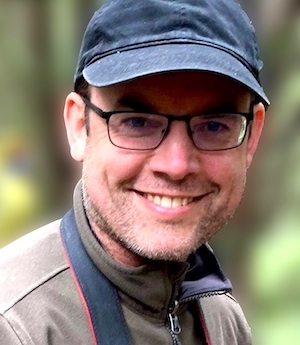
\includegraphics[width=0.25\linewidth]{imagesForRmd/corellaOnShoulder2020croppedBlurredByAdobeOnline}

I thank Hrag Pailian and Lorella Battelli for helpful comments, and also thank Hrag Pailian for providing high-resolution figures of his work.

\hypertarget{objects-that-move}{%
\chapter{Objects that move!}\label{objects-that-move}}

Attention was one of the earliest topics of modern psychology, the science that began in earnest in the late 19th century. William James famously gave us a definition of attention, which began with ``It is the taking possession by the mind, in clear and vivid form, of one out of what seem several simultaneously possible objects or trains of thought.'' This was not just philosophy, as plenty of experiments were being done, using custom apparatus, such as devices that measured response time and presented auditory and visual stimuli.

\begin{figure}
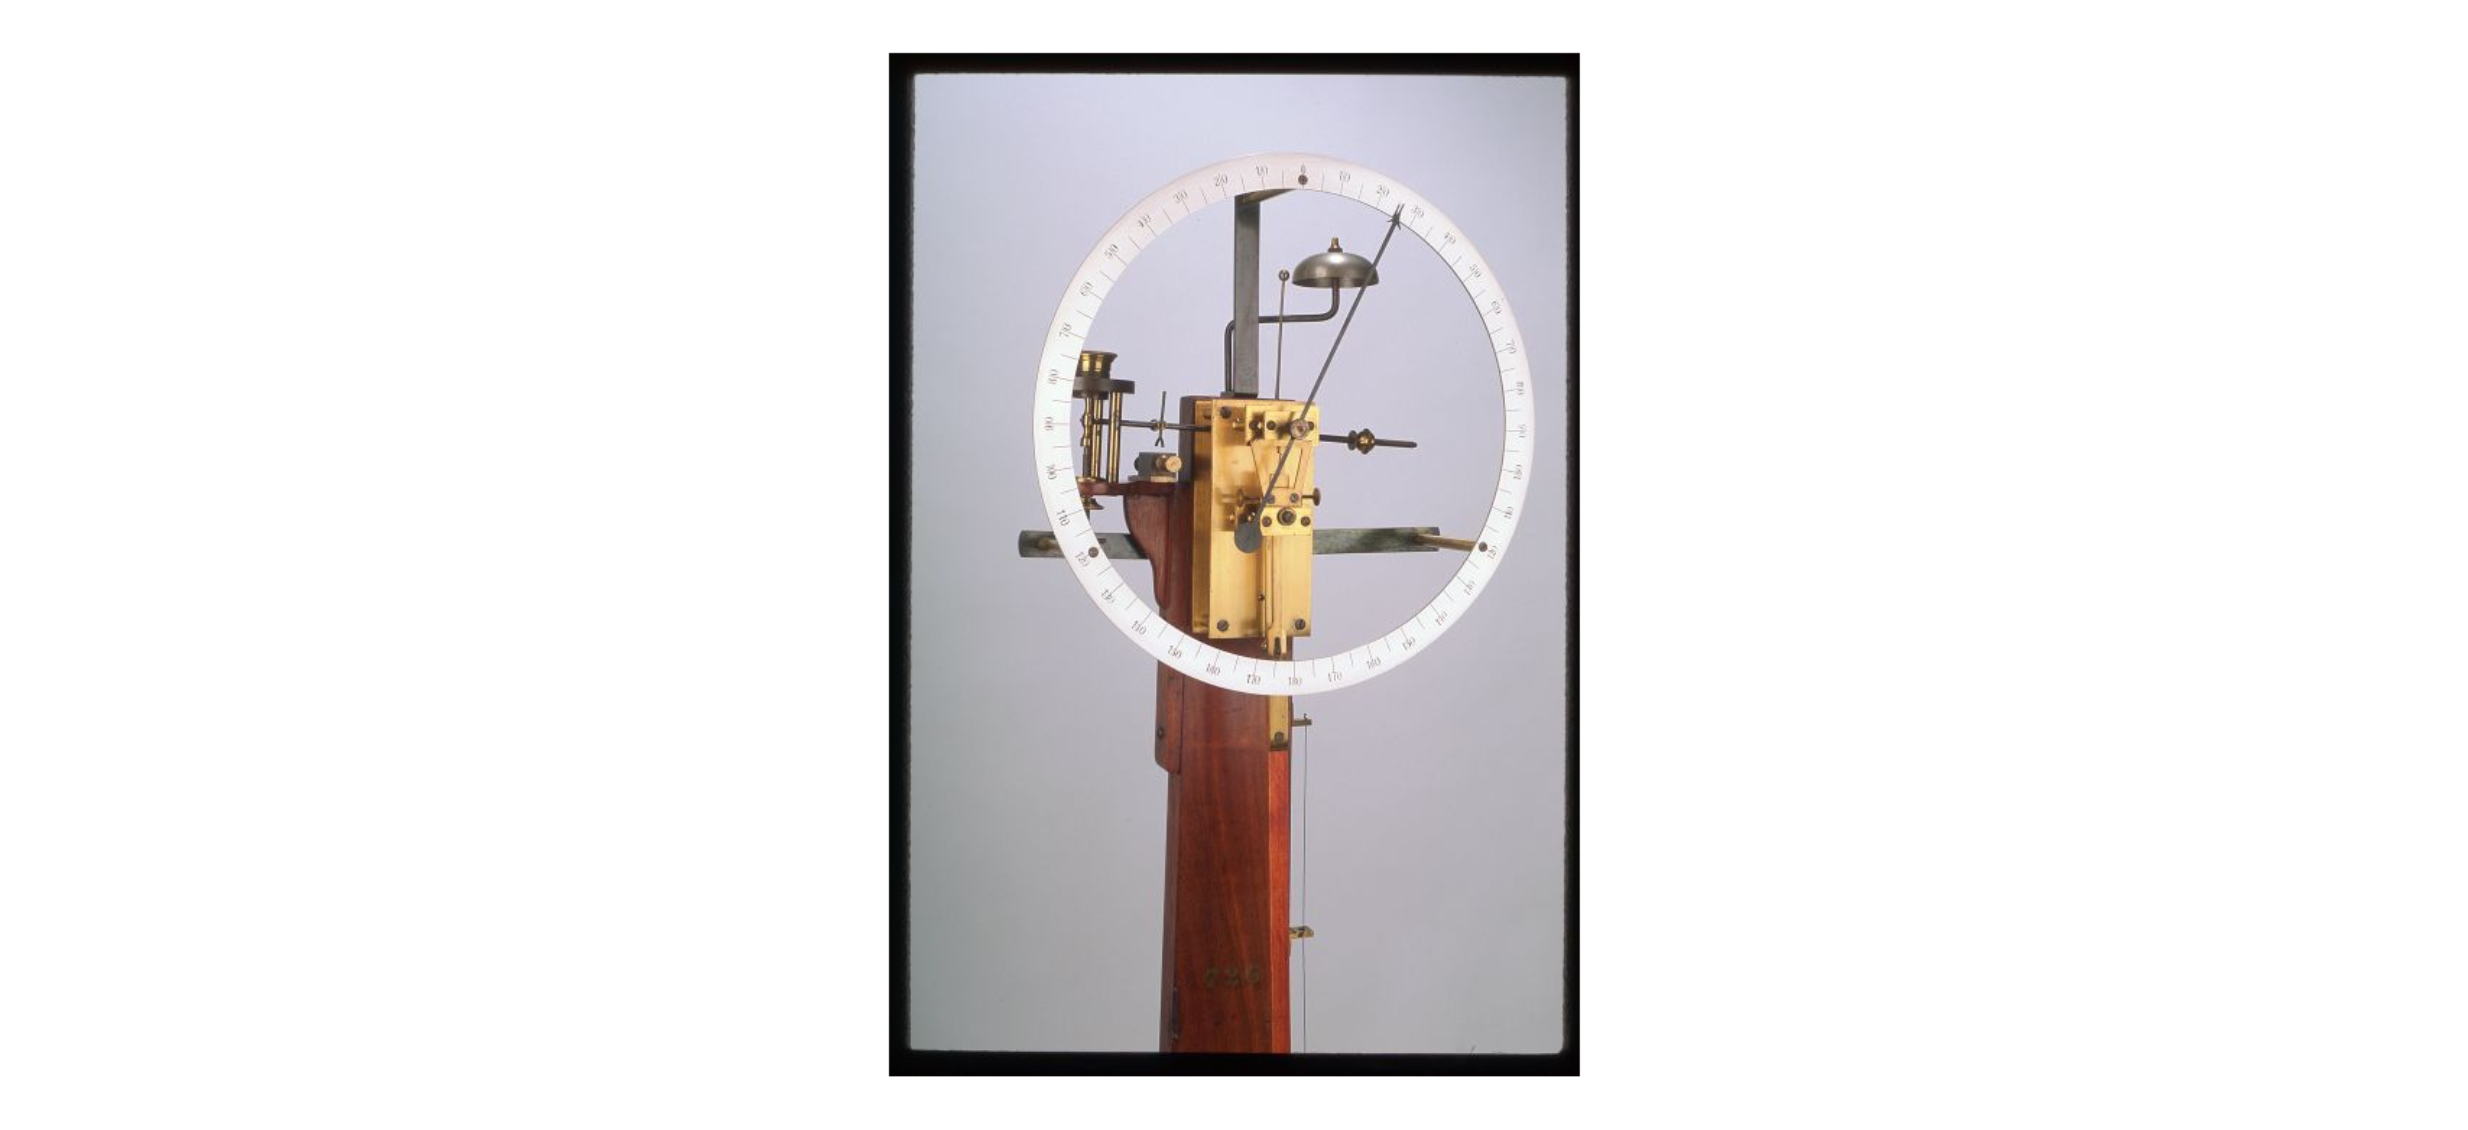
\includegraphics[width=1\linewidth]{imagesForRmd/historical/complicationApparatus} \caption{A 'complication apparatus' from the Harvard laboratory of Hugo Munsterberg. This instrument was used to measure the effect of attention to one stimulus on responses to another.  A subject who focused on one of the numbers on the large dial would have a delayed reaction to the sound of the bell, and vice versa.}\label{fig:complication}
\end{figure}

Munsterberg, one of the first with a laboratory that studied attention, was highly interested in attention and moving stimuli. In his book The Photoplay: A Psychological Study (1916), he presented a theory of cinema, including a twenty-page chapter on attention.

When psychology and the study of attention grew more rapidly after World War II, the study of visual attention was dominated by static stimuli, often stimuli presented briefly with a tachistoscope. Very few researchers used moving objects, and this continued until the 1980s. This was, in part, a technology issue. Scientific laboratories, or psychology laboratories at least, lagged the technology being introduced to arcades and even of homes. In 979, the first popular home game console, the Atari, introduced the game \href{https://youtube.com/embed/YJZ0hB0Vnyk}{Asteroids}.

The point of the game was to shoot and dodge the asteroids that traveled across the screen from all directions. It paid to monitor multiple moving asteroids simultaneously, to determine which way one should move, or shoot, to prevent a collision. Psychologists, however, were slow to take up the programming of computers to present stimuli, and even slower to use them to create moving stimuli.

Psychologists were slow to use the associated technology to study how people attended to multiple moving objects. In the 1970s, however, Zenon Pylyshyn was pondering the possibility of a primitive visual mechanism capable of ``indexing and tracking features or feature-clusters'' (as he put it in \citet{pylyshynTrackingMultipleIndependent1988}; I haven't been able to get copies of his 1970s reports) as they moved. In 1988, \citet{pylyshynTrackingMultipleIndependent1988} programmed an Apple II+ computer to create a display with ten identical objects moving on random trajectories, and connected a telegraph key with a timer to record response times. Finally, he connected an early eyetracker to detect eye movements away from fixation and trigger termination of a trial. Thus he was able to investigate the ability to covertly, without eye movements, keep track of moving objects.

In the experiments of \citet{pylyshynTrackingMultipleIndependent1988}, up to five of the ten moving objects were designated as targets by flashing at the beginning of the trial. The targets then became identical to the remaining moving objects, the distractors, and moved about randomly. It was immediately apparent that people could do this. While viewing the display, one has the experience of being aware, seemingly continually, of which objects are the targets and how they are moving about.

INSERT EXAMPLE MOVIE

But \citet{pylyshynTrackingMultipleIndependent1988} also showed that the processes that underlie tracking are limited in the number of targets that they can faithfully track. Periodically, one of the moving objects flashed, and if the flashed object was a target, the participant was to press the telegraph key. Errors increased fairly rapidly as the number of targets was increased, from 2\% of target flashes missed when only one of the objects was a target, to 14\% of target flashes missed when five of the objects were targets.

Long before Zenon Pylyshyn and Ron Storm devised an experiment to formally document this phenomenon, the notion of kepping track of moving objects was already familiar from everyday life. Any adult who has ever been responsible for more than one child while at the beach or at the park has attempted to continuously monitor the locations of those children. Probably every parent has experienced the sudden panic when, perhaps while chatting with some friends, one realizes that one has lost track of a child. On the sports field, players often concentrate on keeping track of the locations of multiple team-mates, the locations of opponents, and their spatial relationships to the ball. In conference halls, scientists monitor the position and posture of other researchers relative to the ones they are chatting to, in order to best time their approach.

.

You won't find much about tracking in chapters about visual attention. The study of visual attention is still dominated by stimuli that don't move. At the same time, what little most psychology researchers think they know about object tracking is wrong. In this book, we'll bust a few myths about tracking and see that studying it has yielded some unique insights about our limited capacities. To start, we'll lay out a bit about what attention is and why it's interesting.

\hypertarget{outline}{%
\section{Outline}\label{outline}}

\textbf{Intro}

\textbf{Bottlenecks}

\textbf{Which aspect(s) of tracking determine performance?}

\begin{enumerate}
\def\labelenumi{\arabic{enumi}.}
\tightlist
\item
  C=1 processes
\item
  Duration one can sustain attention
\item
  Spatial selection of multiple locations, even static ones
\item
  Spatial interference
\item
  Temporal interference
\item
  Speed limit of attention-following
\end{enumerate}

Each of these could hinder performance more with more targets. They contribute in an unknown mix to most trakcing tasks .
Thus we don't know which is responsible for various results. This has afflicted the quest to understand serialOrParallel,

\textbf{speed, and time.} The physical parameters that can limit tracking performance are space, speed, and time. Each plays a role in different circumstances, but the temporal limits are the most misunderstood, as I have discovered in reviewing journal manuscripts over the years, even though they may be the most fundamental. This section will explain spatial limits, speed limits, and temporal frequency limits on tracking (based in part on three papers from my lab), and how they illuminate other issues such as the relationship of tracking to basic motion and position perception.

\textbf{Serial processing, parallel processing, or both?} The way that our limited capacities are allocated over time to multiple objects, that is whether in parallel or in rapid series, has been a long debate.

\hypertarget{bottlenecks}{%
\chapter{Bottlenecks and capacity}\label{bottlenecks}}

What is fourteen times eleven? You may be able to calculate that in your head, but it would likely take you at least a few seconds to do so. And if I set you two problems rather than just one, for example I asked you to also divide sixty-eight by seventeen, you would do the two problems one at a time. Indeed, our minds may be completely incapable of doing two such problems simultaneously \citep{oberauerAccessInformationWorking2002, zylberbergBrainRouterCortical2010a}.

Such limitations are remarkable given that each of our brains contains more than 80 billion neurons. Simple limitations like these speak to the importance of the architecture of the mind, in particular its bottlenecks, to understanding our abilities.

Multiplying and dividing two-digit numbers are not something that most of us do every day - if we did, perhaps we could do them much faster. A task we do have daily practice with, however, is reading. Yet despite years of daily practice for many of us, a large body of evidence suggests that humans can read at most only a few words at a time, and much research further indicates that we can only read \emph{one} word at a time \citep{whiteEvidenceSerialProcessing2018, reichleEncodingMultipleWords2009}. It seems, then, that at least some of the bottlenecks of human information processing are a fixed property of our processing architecture.

To flesh out the way the word `bottleneck' is used in this context, imagine a standard soft drink bottle. Most of the volume of the soft drink is in the bottom, wide part of the bottle. If one holds the bottle upside-down, most of the contents of the bottle will press down on the narrow neck, and this neck restricts the rate at which the contents can exit the bottle. As a metaphor for the mind, a large volume of signals from across the visual field press up against more limited-capacity brain areas. The large volume of visual signals is crated by the large array of neurons that we have in the retina and a few subsequent areas that process signals in parallel.

The parallel processing prior to the bottlenecks is sufficient to get certain tasks done. In the below display, for example, you should be able to find the blue objects very quickly.

\includegraphics{tracking-review_files/figure-latex/unnamed-chunk-3-1.pdf}

Our visual system processes each of the shapes simultaneously, which can make the locations of the blue objects available very rapidly when you choose to attend to blue. Some brain areas, however, do not have neurons that can recognize objects dedicated to each bit of the visual field. Instead, their simultaneous processing capacity is limited. The processes required to recognize words are one example.

For a limited capacity process such as word recognition to do its job, something is needed to pick out, from a crowded scene, just one or a few objects for these processes to recognize. This something is often referred to as \emph{selective attention}.

Limited-capacity processes impose some of the most severe constraints on human performance. By studying them, we can gain insights into what it is to be human, a conscious create capable of thinking about only a very few things at any one time.

Among visual judgments, word recognition seems to be an extreme case, having a capacity of only about one object \citep{whiteVisualWordRecognition2020}. As demonstrated above, some visual searches reflect processing that can be described as massively parallel, but much other processing falls somewhere in between. That is, the processes underlying some of our abilities are limited in capacity, but not as limited as word recognition seems to be. As we will see, object tracking seems to be one such ability.

That our tracking processes are capable of tracking more than one moving object simultaneously is very useful, because by being aware of the current location of objects of interest, we are able to rapidly deploy all our attentional resources to any one of those locations, allowing more limited-capacity processes to deliver rapid results. When focused attention is applied to an object, that allows even our most limited-capacity processes to operate on the object, which seems to be necessary to, for example, make fine shape discriminations or recognize a word.

A major misconception about object tracking has become widespread, and it relates to the nature of tracking's capacity limit.

\hypertarget{biggestMyth}{%
\chapter{The biggest myth of object tracking}\label{biggestMyth}}

\citet{doranRoleVisualAttention2010} claim that ``the main finding'' from the object tracking literature ``is that observers can accurately track approximately four objects and that once this limit is exceeded, accuracy declines precipitously.'' Similarly, writing about the ``object tracking system'', \citet{piazzaNeurocognitiveStartupTools2010} wrote that ``One of the defining properties of this system is that it is limited in capacity to three to four individuals at a time''. This is a myth.

Two claims are often involved in the myth, but some papers only refer to one of these claims. The first claim is that there is a constant limit of around four objects. The second is that accuracy declines precipitously when the limit is reached. Typically authors do not distinguish between these two claims, instead they make a vague statement that might be taken to refer to either or to both. Here are some examples:
``People's ability to attentively track a number of randomly moving objects among like distractors is limited to four or five items'' \citep{fougnieDistinctCapacityLimits2006}, , ``researchers have consistently found that approximately 4 objects can be tracked'' \citet{alvarezHowManyObjects2007}, ``people typically can track four or five items'' \citet{chesneyEvidenceSharedMechanism2011} , ``participants can track about four objects simultaneously'' \citet{vanderburgChangesNotDifferences2019} . In each of these cases, I have checked the evidence provided, and the papers cited, as well as the papers those cited papers cite. Each paper provides no evidence supporting the claim that performance decreases very rapidly once the number of targets is increased above some value. Those with relevant evidence find only a gradual decrease in performance as number of targets is increased, with no discontinuity; not even a conspicuous inflection point. For example, \citet{oksamaMultipleObjectTracking2004}, which is sometimes cited, designated between two and six objects as targets, among twelve identical objects in total. After the objects moved around randomly for five seconds, one object was flashed repeatedly and participants hit a key to indicate whether they thought it was one of the targets. The proportion of trials in which participants were wrong increased steadily with target size, from 3\% incorrect with two targets, to 16\% incorrect with six targets. Note that even with six targets, participants were performing substantially better than would be expected if they could only track one or two and had to guess on the others.

\citet{pylyshynTrackingMultipleIndependent1988} seems to be the paper most frequently invoked when a limit of four objects is claimed. But \citet{pylyshynTrackingMultipleIndependent1988} found a quite gradual decrease in performance (their Figure 1) as the number of targets was increased from one to five, and five was the most targets that they tested. In their discussion as well, they did not state that there is a hard or precipitous limit. In 1994 however, Pylyshyn and others did write that it is ``possible to track about four randomly moving objects'', even though earlier in that paper they contradict this somewhat by writing ``at least four'' \citep{pylyshynMultipleParallelAccess1994}. I suspect that some cases of this sort of slide toward backing a hard limit reflects a desire for a simple story. It may also stem from an unconscious oversimplification of one's own data, as well as the theoretical commitment of Pylyshyn to the idea that tracking is limited by a set of discrete mental pointers.

Recall that the myth is associated with two claims, not just that there is a ``limit'' after which performance decreases rapidly, but also that this limit is consistently found to be about four. Because the published evidence indicates that the first claim is incorrect, let's put that aside and consider a softer version of the second claim. Specifically, is it the case that tracking performance falls, even if not rapidly, to some particular level, such as 75\% correct, at about four targets? Instead of a percent correct criterion, one might alternatively use a criterion like the halfway point from ceiling to chance performance, or the ``effective number of items tracked'', which is calculated by applying a formula to percent correct together with the number of targets and distractors \citep{schollWhatVisualObject2001}. Charitably, this may be what \citet{alvarezHowManyObjects2007} meant when they wrote: ``researchers have consistently found that approximately 4 objects can be tracked (Intriligator \& Cavanagh, 2001; Pylyshyn \& Storm, 1988; Yantis, 1992).'' To be fair, the cited early studies are arguably compatible with this statement.
However, work published over the last fifteen years has revealed this to be an artifact of researchers using similar display and task characteristics. One of the most salient of these characteristics is object speed.

\citet{alvarezHowManyObjects2007} tested participants with a display of sixteen discs wandering about the screen. They found that the fewer the number of discs they designated as targets, the faster the participants could track each target. In other words, with few targets, participants could track them even when they moved at high speeds. This trend continued as the discs' speed was increased, such that at very high speeds, participants could track only one object with reasonable accuracy. This indicated that the truth of the idea that participants can track four objects is entirely dependent on the speed of those objects. Supporting evidence for this was found by my lab \citep{holcombeExhaustingAttentionalTracking2012}.

Soon, other display parameters that affect the number of objects that can be tracked were discovered, in particular object spacing \citep{franconeriEvidenceSpeedLimit2008, holcombeObjectTrackingAbsence2014}. As we will be discussed extensively in section \ref{twoBrains}, one aspect of spacing is that tracking performance can depend greatly on whether the targets are distributed between the left and right hemifields or instead are confined to one hemifield.

In summary, it is incorrect to say that people can track about four moving objects, or even that once some number of targets is reached, performance declines very rapidly with additional targets. The number that can be tracked is quite specific to the display arrangement, object spacing, and object speeds. If a researcher is tempted to write that ``people can track about four objects'', the immediate context ought to stipulate that this refers to certain tasks, display characteristics, and performance measures, something that I have almost never seen in the literature.

Almost exactly this issue also arose in a different research area. A diverse set of two dozen working memory researchers attended a workshop in 2013 with the express purpose of ``developing benchmarks for models of working memory''. They grappled with, among other issues, how to characterize the limit on how many items people can remember. In a paper that stemmed from the discussions at the workshop, the researchers pointed out that ``observed item limits vary substantially between materials and testing procedures'' \citep{oberauerBenchmarksModelsShortterm2018}. However, they suggested that much of this variability could be explained by humans' ability to store groups of items as ``chunks'' and thus the group endorsed a statement that there is a limit of ``three to four chunks'' \citep{cowanMagicalNumberShortterm2001a}. These researchers believed they could explain the observed variability in experiments' results by a common underlying limit of three to four chunks that manifests as different observed item limits depending on circumstances, in particular the opportunity for chunking.

In the case of MOT, it remains possible that researchers will be able to identify a set of circumstances that consistently yield a mean tracking limit of three or four targets (if ``limit'' is defined as performance falling to a particular level on some performance metric). Perhaps these circumstances will simply be certain spacings, speeds, object trajectories, and number of objects in a display. Ideally, however, some underlying construct (the counterpart of chunks for memory) would be identified to explain how performance changes when other circumstances are used. That would constitute real progress in theory development. However, I don't see anything like that in the literature currently.

\hypertarget{different-tasks-same-limit}{%
\section{Different tasks, same limit?}\label{different-tasks-same-limit}}

Even with the idea that there is a particular number of objects one can track discarded, there remains a related claim, one common in the literature, that conceivably could still be viable. This claim is frequently tangled up in the myth reviewed above, for example it may be stated as the idea that there is a ``magical number four''. After discarding the attachment to a particular number, the essential notion is that very different tasks have the same number-of-objects limit. For example, \citet{bettencourtSharedFilteringProcesses2011} stated that ``both processes {[}visual short-term memory and MOT{]} showing an equivalent four-object limit'', and \citet{piazzaNeurocognitiveStartupTools2010} similarly claimed that visuo-spatial short-term memory, ultra-rapid counting (subitizing), and multiple object tracking all share a limit of ``three or four items''.

For more than a hundred years, it has been claimed that there is a discrete limit on the number of objects that can be, at a glance, counted \citep{jevonsPowerNumericalDiscrimination1871}. This ``subitizing'' or numerosity perception ability has been extensively investigated, and some consider the idea of a sudden decrease in accuracy when the number of objects shown goes from less than four to more than four as well-supported \citep{revkinDoesSubitizingReflect2008}. Four objects and fewer is frequently referred to as the ``subitizing range'', with performance approximately as good for rapidly counting four objects as it is for two or one. Note that this is very different than in tracking, for which speed thresholds decline rapidly from one to two targets, as well as to three and four. For visual working memory, which as we mentioned several experts have characterized as being limited to three or four chunks, whether there is a discontinuity after four objects or at any point remains highly debated \citep[e.g.][]{robinsonThereCapacityAssessing2020}.

At the level of a common limit in terms of number, then, it remains unclear whether tasks such as object tracking, visual working memory, and subitizing can be said to have a common limit. Ideally this could be confirmed by measuring the limits for all three tasks using the same stimuli, but it is unclear how to equate the information available across tasks. Especially difficult is comparing performance with the briefly-presented static stimuli used in subitizing and working memory tasks to the extended exposures of moving stimuli needed to assess object tracking. A modeling approach could make progress on this issue, although it would require making assumptions that might need novel empirical support. Another approach is to determine which tasks' limits co-vary between individuals. This is reviewed in section \ref{abilities}.

To summarize this chapter, there are three common misconceptions about what has been shown about object tracking. The one that we have just discussed is that different tasks show the same limit. This may actually be true, but I know of no research that have used the same display and task settings to adequately back this up. In the previous section of this chapter, we saw that it is not justified to say that as the number of targets is increased to about four, performance falls to a certain criterion level. One must specify particular display and task characteristics in order to make that statement true. A final misconception is that performance falls very rapidly when one increases the number of targets past a particular number (the ``limit'').

Given that tracking performance does depend greatly on circumstances and falls gradually rather than displaying a discontinuity at a particular target number, what are the implications for how tracking works? Briefly, these characteristics of tracking are consistent with resource theories, which are discussed in Chapter \ref{whichAspects}.

\hypertarget{objects}{%
\chapter{Objects and attentional spread}\label{objects}}

As I sit in my cluttered living room, sunlight streaming through the window illuminates dozens of objects that reflect light into my retinas. The family dog, which had been napping, gets up and ambles into the kitchen. As he moved, I tracked him with my attention. To do so, something in my brain had to identify a changing set of neurons, responding to different parts of the moving dog, as constituting one object. What sort of processing is involved?

It starts in the retina, but the processing that occurs there is far from enough to segment a dog, or practically any other object, from my living room background. Processing in the thalamus and early visual cortex, at the very least, continues the job. Much, or perhaps all, of this early cortical processing occurs regardless of where one is attending. Exactly how extensive this ``preattentive'' processing is, and what sorts of representations it results in, has been studied for a while, but much is still not understood \citep{neisserDecisionTimeReactionTimeExperiments1963, treismanVerbalCuesLanguage1964, kimchiFiguregroundSegmentationCan2008}.

Attentive tracking is often conceptualized as a process wherein a limited resource simply selects one or more of the preattentively-created representations. In fact, it is unclear whether processing is so neatly divided, with preattentive representations merely selected rather than attention participating in modifying or even creating the representation that is tracked. For example, a popular view is that attending to a location results in binding some of the features there, such as color and orientation, but attention likely also contributes to figure-ground segregation, a more fundamental aspect to defining an object \citep{petersonLowlevelHighlevelContributions2014}. \citet{nakayamaDynamicNoiseBackground2021} even suggested, in order to explain the twinkle-goes illusion, that attentional tracking could cause the representation of a moving object to persist after the object has disappeared.

With behavioral tasks, perhaps the most straightforward assessment that can be done is to investigate which sorts of stimuli can be tracked and which cannot. The first deployment of attention to a stimulus likely occurs more via a spatial or featural index than through an index of the objects in the scene. We cannot think ``car'' or ``tree'' to ourselves and expect our attention to deploy directly to any cars or trees in the scene. In contrast, our ability to deploy attention to a cued, static \emph{location} is well-established, as is our ability to deploy attention directly to certain other features, such as color or motion direction. When people are instructed to think about a particular location in the visual field, this results very rapidly in facilitation of perceptual performance for that location, and neural activation in the associated parts of retinotopic cortices. No "search process seemss to be needed, instead spatial location seems to provide a direct conduit for attentional activation. Similarly, for certain features such as motion or color, an instruction to attend to a particular direction, or a particular color, triggers rapid activation across the visual field at all the locations of that color or motion \citep{saenzGlobalFeaturebasedAttention2003, whiteFeaturebasedAttentionInvoluntarily2011}.

As a result of this featural selection capability, if a moving target differs from distractors in certain ways, then featural selection can be relied on to keep attention on the target. For example, if the targets are the only yellow objects in the scene, and all the distractors are blue or green, then one can think ``yellow'' and that is enough to keep attention on the targets and off the distractors (this will come up again in Chapter \ref{identity}). It is when the targets are identical to the distractors, or not distinguishable from the distractors by one of the features that feature selection acts on, that a different process is needed to keep attention on a moving target.

When the targets and distractors are identical, spatial location selectio may initiate the selection of a target, but if it were the only process operating, when an object moved, attention would be left behind. And a striking characteristic of the experience of tracking is that the movement of attention along with an object feels like it takes no more effort than selecting a static object. Indeed, one might say that attention seems to be positively pulled along - when the targets in an MOT trial begin to move, I have never had the experience of my attention staying behind, remaining at one of the original target locations. It feels unnatural to un-latch my attention from a target and fix it to the target's current location while the target moves on.

The term ``object-based attention'' is sometimes bandied about as an explanation of why attention seems to automatically move along with a selected object, the idea being that the units of selection are objects rather than locations \citep{pylyshynSeeingVisualizingIt2006, clarkLocationLocationLocation2009}. But no one seems to think that direct selection of objects is a thing, in the way that color selection is. That is, one cannot think ``chair'' and have all the locations of chairs in the scene become rapidly attended. Selection of chairs, or another object type, seems to require a search first, based on locations and simpler features. And even color selection may work via location, with thinking of a color resulting in availability of its locations, and attention then being deployed to those locations \citep{shihThereFeaturebasedAttentional1996a}.

One notion that fits in with these considerations is that attention is deployed first to a location or locations, but any object present can cause spatial attention to spread throughout that object. Although researchers who study the relationship between attention and objects often are not explicit about their theory, this ``attentional spread'' theory seems to be a popular one.

\hypertarget{stationary-object-selection}{%
\section{Stationary object selection}\label{stationary-object-selection}}

Dozens, possibly hundreds, of published papers have investigated the relationship of objects to attention, using a particular kind of cuing paradigm. It all started with \citet{eglyShiftingVisualAttention1994a}, who presented two static objects (rectangles) and presented a cue on one end of an object or another. They found that the cue could result in a performance enhancement not only for probes at the location of the cue, but also at the cued object's other end (measured relative to equidistant locations on the second object). The findings reported in most of the many follow-up papers similarly find that participants are fastest and most accurate when the stimulus is presented in the same location as the cue, or on the same object but on a different part of that object. I used the qualifier ``most'' when referring to the follow-up papers because some papers did not find this \citep{davisReversalObjectBased2005, shomsteinObjectbasedAttentionStrength2008, shomsteinObjectbasedAttentionSensory2002, louIndividualDifferencesTemporal2020}, and a major concern is that studies that did not find an advantage were more likely to end up in the proverbial file drawer. In particular, the effect sizes in the literature are often quite small and the studies not highly powered, which can be a red flag that publication bias may have created the illusion of a real effect \citep{buttonPowerFailureWhy2013}.

\citet{francisExcessSuccessArticles2021} assessed the pattern of sample sizes, effect sizes, and p-values in three dozen published object-based attention studies and argue that it suggests that publication bias and/or p-hacking in the literature is rife. This is plausible, because substantial proportions of researchers in psychology and other fields admit to such practices \citep{johnMeasuringPrevalenceQuestionable2012, rabeloQuestionableResearchPractices2020, chinQuestionableResearchPractices2021}. \citet{francisExcessSuccessArticles2021} further point out that the only previously-published study with a large sample (120 participants) found a non-significant effect of only a 6.5 ms difference in response time \citep{pilzHowPrevalentObjectBased2012}, and in their own study with 264 participants, the effect was also quite small, at 14 ms. For an effect of this size, the sample sizes typically used in the published literature were unlikely to yield statistical significance without some help from p-hacking or another questionable research practice. As a result, many papers in the literature make conclusions about objects and attention based on results that unfortunately cannot be trusted.

Publication bias and p-hacking plague many areas of the psychological literature. They are less of an issue when the effects being studied are large, because in those cases studies are more likely to be adequately powered, resulting in fewer false positives and false negatives. The study of object tracking is fortunate that its subject matter has yielded several large and robust effects. Some are so large that spending a period of seconds looking at a display is enough to convince oneself that an effect is real. Those very large effects include some that relate to how variation in objects affects tracking.

\hypertarget{the-end-of-the-line}{%
\section{The end of the line}\label{the-end-of-the-line}}

Many objects, such as the letter `T', are comprised of salient parts. Normally we think of `T' as a single object, but we can also see that it is made up of a horizontal segment as well as a vertical segment. In conscious awareness, then, we have access to both the whole object level and to an individual parts level. You are able to focus attention on individual bits of the vertical segment, even though there are no visual characteristics that differentiate it. But which level(s) does our object tracking processes operate on?

In early visual cortex, different populations of neurons respond to the the horizontal and to the vertical stroke of a `T'. But having neurons that respond to a thing does not suffice to be able to track that thing. Only particular kinds of neural representations enable tracking.

\citet{schollWhatVisualObject2001} shed light on this by asking participants to try to track the ends of lines. Participants were presented with four lines, with one end of each line designated as a target. After the movement phase, at the end of the trial participants were to click with a mouse on the line ends that were targets. During a trial, each line grew, shrank, and rotated as each of its ends wandered about the screen randomly.

The notion that one end of an undifferentiated shape is an object is somewhat unnatural. It can be useful, however. When paying attention to someone holding a rifle, for example, it may be important to continuously monitor the direction that the front of the gun is pointing.

\begin{figure}
\centering
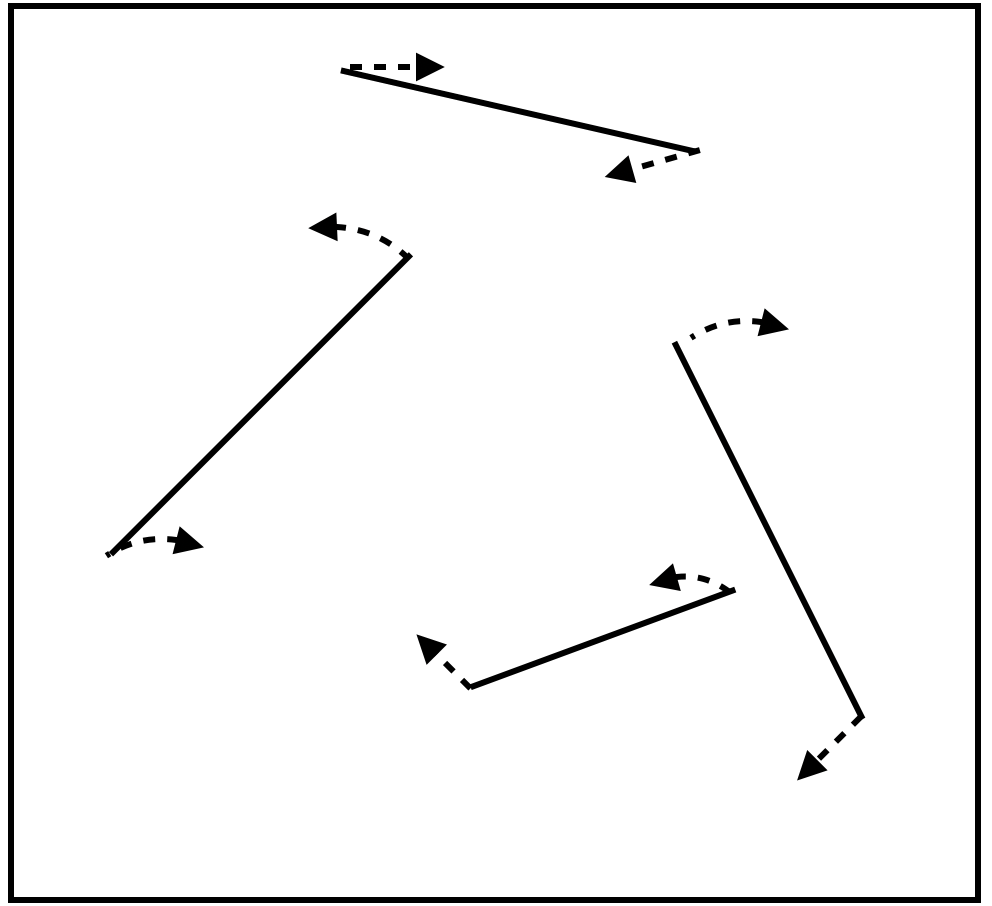
\includegraphics[width=0.4\textwidth,height=\textheight]{imagesForRmd/linesSchollPylyshynFeldman_madeByHolcombe.png}
\caption{A schematic of the display used by Scholl et al.~(2001)}
\end{figure}

The results were striking. Performance on the task was abysmal relative to a control condition in which the two ends of the line were not connected. Simply by viewing an example trial, one very quickly gets a sense of how difficult the task is - the effect is very large.

(ASK SCHOLL FOR THE MOVIE RIGHTS)

The task of tracking line ends in the experiment of \citet{schollWhatVisualObject2001} experiment was complicated by the fact that the objects frequently crossed over each other and also their length changed over time, raising the question of whether these factors were the reason why tracking was difficult. Follow-up work by \citet{howeCanAttentionBe2012}, however, showed that these were not the main reason for the poor performance. It simply is the case, it seems, that one cannot confine one's tracking processes to one bit of an undifferentiated object.

Our inability to track the ends of lines fits in with the view this chapter opened with, that preattentive processes define objects that become what tracking operates on. This relates to an aspect of experience with static images. Maintaining attention on a part of the visual scene in the absence of anything in the image to delineate that part \emph{feels like} it requires concentration, as if we must continually think about what we are supposed to be attending to. If lots of cognitive resources are needed to maintain the ``object'' representation when it is not provided by preattentive processes, it is possible that one can track a single target but not more. This idea of C = 1 (capacity of one) processes being involved or required for some forms of tracking is discussed more in \ref{whichAspects}.

\hypertarget{object-creation-and-object-tracking-distinct-processes}{%
\section{Object creation and object tracking: Distinct processes?}\label{object-creation-and-object-tracking-distinct-processes}}

Conceptually, researchers distinguish between the processing that determines \emph{how many} objects one can track and those that determine \emph{what kinds} of objects can be tracked. But do these things happen in different processing stages, or do they interact? An assumption of separate processing stages is popular in the study of visual cognition generally. Visual search, for example, is usually conceptualized this way \citep{wolfePreattentiveObjectFiles1997, nakayamaVisualSurfaceRepresentation1995}, and appears to be an implicit assumption in two reviews of objects and tracking \citep{schollObjectsAttentionState2001, pylyshynSeeingVisualizingIt2006}.

\begin{figure}
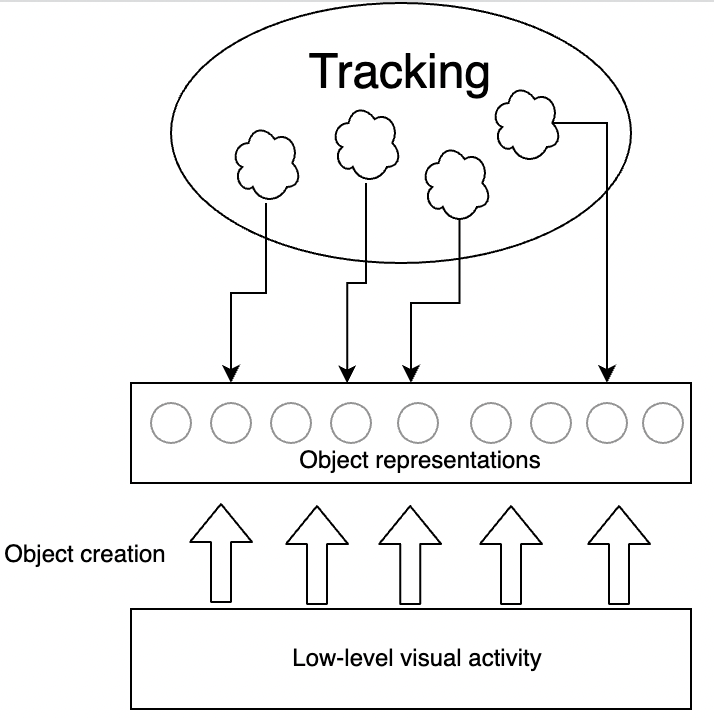
\includegraphics[width=0.3\linewidth]{imagesForRmd/flowDiagrams/objectCreationTrackingSeparateDiagram} \caption{A schematic of the idea that objects are created prior to the action of tracking processes, which then point to the already-formed object representations but do not change them.}\label{fig:simpleArchitecture}
\end{figure}

It would be convenient if object creation and object tracking occurred at distinct processing stages, as that is straightforward relative to an interactive system \citep{simonSciencesArtificialReissue1969, sternbergDiscoveryProcessingStages1969}. And there certainly is evidence that tracking is high-level, for example \citet{maechlerAttentionalTrackingTakes2021} found evidence that tracking operates on perceived object position rather than more low-level representation of position.

There is evidence, however, that attention and object creation are interactive. For example, the way stimulus elements are organized by attention can determine what illusory contours are created and perceived, as well as the lightness and depth that is perceived \citep{harrisonVoluntaryControlIllusory2019, harrisonAttentionalSelectionIllusory2019, peterVoluntaryAttentionModulates2005}. Our ability to perceive the complex motion of a human body from only several points of light highlights that object perception can involve hierarchical motion segmentation that reflects an interaction between Gestalt grouping and top-down knowledge of the overall shape of objects and the relative motion pattern of their parts \citep{johanssonJohanssonVisualPerception1973, wangSearchingLifeMotion2010} (see the grouping Chapter (\ref{grouping})).

Using a paradigm based on that of the attentional spread literature reviewed above, \citet{ongchocoHowCreateObjects2019} asked participants to practice ``seeing'' certain shapes in a uniform grid of lines. The detection of flashed probes was enhanced for those presented on the same (purely imagined) object, compared with equidistant ones presented on different objects. In summary, a variety of evidence suggests a role for neural feedback in object segmentation, with some role for attention, but the extent of its importance remains unclear \citep{papaleInfluenceObjecthoodRepresentation2021, wyatteEarlyRecurrentFeedback2014, harrisonVoluntaryControlIllusory2019}.

Potentially, the same attentional resources that mediate tracking may also contribute to the creation of object representations. One consequence would be a trade-off between the involvement of attention in constructing object representations and the number of objects that can be tracked. Informal experience with tracking the line ends in the \citet{schollObjectsAttentionState2001} display seems to support this. If when you watch the SCHOLL MOVIE, you concern yourself with keeping track of the end of only \emph{one} object, you are likely to succeed. But recall that it is difficult or impossible to accurately track \emph{four} object ends - indeed, \citet{schollObjectsAttentionState2001} found that participants' performance was approximately that predicted if they could track one line end, but not more. This finding is consistent with the notion that some aspects of object creation tap the same attentional resource as tracking does.

An important alternative, however, is that our minds harbor a tracking resource that can be brought to bear on one object, but not multiple objects. This would mean that covert tracking of multiple objects is qualitatively different from covert tracking of a single object. It may seem unparsimonious to posit this, but in fact there seems there is both a hemifield-specific tracking resource and a more global resource. This is discussed further in \ref{twoBrains}.

\hypertarget{what-tracking-sticks-to}{%
\section{What tracking sticks to}\label{what-tracking-sticks-to}}

Even when all of our cognitive resources are brought to bear on a single entity, some sorts of entities still can't be tracked. \citet{anstisEyesPursueMoving2010} asked participants to track the intersection of two shapes, a configuration that causes the ``chopsticks illusion'' \citet{anstisImperceptibleIntersectionsChopstick1990}. In the ``chopsticks illusion'', a horizontal and vertical line slide over each other, each following a clockwise circular trajectory. Viewers perceive the intersection of the two lines to also be moving clockwise (demo \href{http://anstislab.ucsd.edu/illusions/chopsticks-illusion/}{here}), but in fact the intersection moves only counterclockwise. This seems to be, in part, a failure of object tracking because if participants had been able to attentionally track the intersection, they should have been able to judge its trajectory. Moreover, \citet{anstisImperceptibleIntersectionsChopstick1990} found that participants could not accurately pursue the intersection with their eyes. The true counterclockwise trajectory of the intersection becomes obvious perceptually if one views the display through a window so that the ends of the lines are occluded rather than visible, and in that condition participants could smooth pursue the intersection accurately. \citet{anstisImperceptibleIntersectionsChopstick1990} believe the reason that the intersection is ordinarily perceived to move in the wrong direction is because the clockwise motion of the ends of the lines is mistakenly assigned to the intersection, similar to how the motion of the ends of lines causes the barber-pole illusion. Regardless of the cause of the illusion, it constitutes a failure to track a rather simply-defined point. Evidently, a particular interpretation of motion and form was created and tracking could not effective operate on the simpler intersection of the lines. As schematized by the figure above, certain processing of motion and form appears to occur prior to the operation of tracking.

\begin{figure}
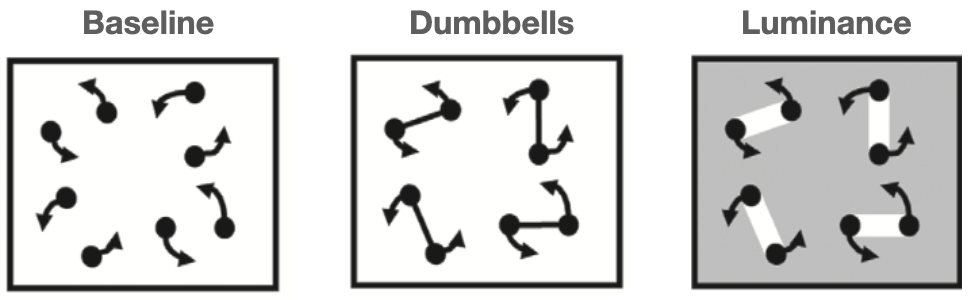
\includegraphics[width=1\linewidth]{imagesForRmd/PiersHowe/PiersHoweStimuli} \caption{Some stimuli used by Howe et al. (2012). CC-BY}\label{fig:unnamed-chunk-4}
\end{figure}

``The ends of the line'' section above described the finding that people can't track the ends of multiple objects. Evidently, maintaining the representation of an undifferentiated part of an object is not something that our multiple object tracking resources are capable of. What sort of differentiation is needed? \citet{schollWhatVisualObject2001} varied how distinct the end of an object was. In a ``dumbbell'' condition, each object was simply two squares connected by a line. In that condition, participants' accuracy was lower than the original separate squares condition, but not statistically significantly so - any detriment to tracking appeared to be small, suggesting that participants could track a dumbbell end. However, \citet{howeCanAttentionBe2012} also used a dumbbell condition that was rather similar to that of \citet{schollWhatVisualObject2001}, but they found performance was substantially lower than when the objects (which were discs in their case) were not connected. The reason for the discrepancy is not clear, and it appears it could reflect the noisiness of the data of the two studies. \citet{howeCanAttentionBe2012} also tested a ``luminance'' condition, pictured above, and found that performance (80\% correct) was substantially lower than their baseline condition (96\% correct), although not as low as for undifferentiated bar ends (72\% correct). They were surprised that the clear difference in luminance between the targets and the connector in the luminance condition was not enough to keep tracking from being so adversely affected by the connectors.

These results suggest that multiple object tracking uses a more ``primitive'' segmentation of objects than what is available to us when we focus our attention on a single object. These findings have some similarity to those found in conjunction visual search studies. \citet{wolfePreattentiveObjectFiles1997}, for example, asked participants to search for conjunctions of features, such as red and vertical. If the vertical red part of an object were physically connected to a horizontal and green part, then participants were much slower to find the red vertical target segment in the display, among the green vertical and red horizontal distractors. In other words, it seemed that physically connecting one feature to another lumped it together as an undifferentiated collection of features from the perspective of search processes, what \citet{wolfePreattentiveObjectFiles1997} termed a ``preattentive object file''. Although to my knowledge, no researcher has tested displays of this nature for both tracking and search , the parsimonious account has to be that multiple object tracking and search operate on the same object representations.

\hypertarget{growth-shrinkage-and-tracking}{%
\section{Growth, shrinkage, and tracking}\label{growth-shrinkage-and-tracking}}

In the real world, some objects and substances change shape. When one opens a faucet in a kitchen, for example, a jet of water will shoot into the sink, and flatten on the sink's bottom, rapidly expanding into a puddle. As one pours beer into a glass, a froth forms, which gradually thickens as the top of the liquid rises. These are examples of non-rigid motion, in these cases substances that change shape as they move.

To investigate tracking of non-rigid substances, \citet{vanmarleAttentiveTrackingObjects2003} devised an object that resembled an inchworm or slinky. In a condition I will refer to as the ``slinky'' condition, each object began as a square. It would then move by extending its leading edge until it had the shape of a long and thin rectangle. Subsequently, the trailing edge of the slinky, which was still at its original location, would retract until the slinky was a square again, now entirely at a new location. In this condition, tracking performance was very poor. What is it about tracking that causes such difficulty with slinkys? \citet{howeVisuallyTrackingLocalizing2013} tested a number of conditions that ruled out issues such as the faster speed of the slinky's edges relative to the control conditions.

\citet{schollWhatHaveWe2008} suggested that the reason the slinky was difficult to track was that ``there was no unambiguous location for attention to select on this shrinking and growing extended object'' because ``each object's location could no longer be characterized by a single point'' (p.63). There may be something to this, but it is not entirely clear what is meant by an object's location not being characterizable by a single point. Consider the canonical objects used in this literature - discs with no internal features. They also have no unambiguous internal locations, because their insides are a completely undifferentiated mass. If one wishes to refer to a single point for their location, their centroid could be used, but this seems just as true for an object changing in size and shape. Additionally, in the chopsticks illusion reviewed above, the target was defined by a single point (the intersection of two lines), but it also could not be tracked.

Although the reason remains obscure, it seems that object expansion and contraction disrupt not only tracking, but also localization. \citet{howeVisuallyTrackingLocalizing2013} replicated the tracking results of \citet{schollWhatHaveWe2008}. They also investigated further, presenting a rectangle for 200 ms at a random location on the screen, and asking participants to click on the location of the center of the rectangle. In a baseline condition, the rectangle did not change in size, shape, or location during its 200 ms presentation. In the size-change condition, the length of the object increased due to expansion for half of the interval and shrank due to contraction during the other half. Participants' localization errors were about 14\% larger in this changing-size condition. This appeared to be driven by errors along the axis of the object's expansion and contraction, as errors in the orthogonal direction were not significantly different from the baseline condition.

The localization impairment documented by \citet{howeVisuallyTrackingLocalizing2013} was substantial, and thus may yield the very low performance when participants attempt to track multiple slinkys. However, it still is not clear whether the localization impairment is large enough to account for the very low tracking performance. An important next step is to measure localization errors when the task is to monitor multiple objects changing in size rather than just one. If the localization deficit caused by change in size worsens with object load, this would help implicate the processes underlying tracking .

\hypertarget{could-tracking-work-by-attentional-spreading}{%
\section{Could tracking work by attentional spreading?}\label{could-tracking-work-by-attentional-spreading}}

The relationship between object representations and tracking pictured by Figure \ref{fig:simpleArchitecture} suggests that attention selects entire object representations, as a whole. It has been suggested, however, that he process instead begins by selecting a particular location, and then selection spreads up to the edges of the object. A gradual growth of the area of attentional activation to encompass an entire object has been observed neurophysiologically in certain tasks \citep[e.g.,][]{wannigAutomaticSpreadAttentional2011}.

The spreading of attention could conceivably explain the ability to keep attention on multiple moving objects. When an object moves, if it moves smoothly, then its leading edge will occupy new territory while its trailing edge continues to occupy an old location. If spreading of attention up to object boundaries is continually occurring, then attention should spread to the new locations near the trailing edge. In such a fashion, attention could, by continually expanding to the new location of a leading edge and contracting with a trailing edge, stay on a moving object. However, the neural spreading process observed neurophysiologically seems too slow to keep up with fast-moving yet trackable objects.

Behavioral results from presenting probes at various locations inside and outside of moving targets adds to the complexity here. Presenting probes during a task of tracking multiple lines, \citet{alvarezHowDoesAttention2005} found that probes presented at the center of objects were detected much more accurately than end probes, suggesting that attentional resources were concentrated on the centers of the lines. The spreading account seems to instead predict that accuracy would be highest near the trailing end of an object. It appears, however, that the researchers did not analyze the data to check whether of the two object ends, accuracy was higher for probes at the trailing end. Clearly, much more work is needed to reveal the nature of attentional spread while an object moves and any role that has in facilitating tracking.

\hypertarget{grouping}{%
\chapter{Grouping}\label{grouping}}

Carving the scene into objects is not the only form of visual segmentation that our brains perform. We perceive groups formed by a variety of cues. This suggests that tracking might follow entire groups rather than individual elements of a group. \citet{alzahabiEnsemblePerceptionMultipleobject2021} used clusters of several discs as targets and distractors. These clusters maintained a constant spatial arrangement as they wandered about the display. Participants seemed to do well at tracking these clusters. Unfortunately these researchers did not rule out the possibility that participants were tracking just one disc of each cluster, however, and I am not aware of any work that provided strong evidence that a tracking focus tracks an entire group.

\citet{yantisMultielementVisualTracking1992} hypothesized that in MOT experiments, participants track an imaginary shape formed by the targets, specifically a polygon whose vertices are the target positions. Progress has been slow in understanding whether all participants do this or just a minority do, and in what circumstances. \citet{merkelSpatiotemporalPatternsBrain2014} found a result that they took as evidence that some participants track a shape defined by the targets while others do not. In their task, when the targets and distractors stopped moving at the end of the trial, four of them were highlighted again and the task was to press one button if all four were targets (match), and to press a different button otherwise (non-match). Error rates were lowest when none of the objects highlighted were targets, and errors were progressively more common as the number of highlighted objects that were targets increased. This was unsurprising. However, for trials where all four of the highlighted objects were the targets (match), error rates were much lower than when only three were targets. \citet{merkelSpatiotemporalPatternsBrain2014} suggested that this reflected a ``perceptual strategy of monitoring the global shape configuration of the tracked target items.'' They went on to split the participants based on whether they had a relatively low error rate in the match condition, investigated the neural correlates of that, and made various conclusions about the neural processing that underlies virtual shape tracking.

These inferences of \citet{merkelSpatiotemporalPatternsBrain2014} are all based on the split of participants based on low error rate in the match condition compared to the condition where none of the highlighted objects match. The idea seems to be that if participants weren't using a shape tracking strategy, error rates would steadily increase from the trials where none of the highlighted objects were targets to the trials where all of the objects highlighted were targets. However, there are other possible reasons for this pattern of results.

One aspect of the \citet{merkelSpatiotemporalPatternsBrain2014} experiment is that one of the two response choices (non-match) was the correct answer in 80\% of trials. Because participants were not told that, some of them surely expected that they should press the two buttons approximately equally often. By pressing the match button more often (close to 50\% of trials) than the appropriate 20\% of trials, they would artificially have the relatively low error rate for the full-match condition that was observed. \citet{merkelSpatiotemporalPatternsBrain2014} mention the possibility of a response bias but suggest that this would result in the opposite (a high error rate) to what I have suggested. The problem seems to be that they didn't consider that the participants may have expected the match stimulus to occur more often than it did.

A response bias is not the only alternative to the virtual grouping account of \citet{merkelSpatiotemporalPatternsBrain2014}. The low error rate in the full-match condition might also occur for other reasons. Imagine that a participant tracked only one target and simply checked that target at the end of each trial for whether it was highlighted. If that one target is not highlighted, the participant presses the non-match button, otherwise they press the match button. For such a participant, the chance of getting the answer wrong when none of the probed objects are targets is zero. It is higher when one of the probed objects is a target (25\% if the participant tracks one target perfectly on every trial and makes no finger errors), and still higher when two or three probed objects is a target. When three probed objects are targets, in three out of four cases, one of them is the target the participant tracked, so the participant frequently gets it wrong. But when all four of the probed objects are targets, the participant will always respond correctly. Thus, a low error rate in this all-targets-probed condition that is very close to the error rate in the no-targets-probed condition can be a sign of a participant who only monitors one target. But \citet{merkelSpatiotemporalPatternsBrain2014} interpreted this result as instead meaning that the participant was tracking a virtual shape formed by all four of the targets.

\hypertarget{hierarchical-relations}{%
\section{Hierarchical relations}\label{hierarchical-relations}}

In the real world, the movement of a scene relative to our retinas is rarely as independent as the moving objects in a typical multiple object tracking experiment. Often there is a strong motion element throughout the visual field created by the movement of the observer, and recovering true object movement likely requires detecting deviations from that \citep{warrenPerceptionObjectTrajectory2007}. Even when the observer is completely still, hierarchical motion relationships are common. When one views a tree on a windy day, the largest branches sway slowly, while the smaller limbs attached to the larger branches move with the larger branches but also, being lighter, have their own, more rapid motion.

These aspects of the structure of the visual world may be one reason that our visual systems are tuned to relative motion \citep{tadinWhatConstitutesEfficient2002, maruyaRapidEncodingRelationships2013}. When we see a wheel roll by, we experience individual features on the wheel as moving forward, reflecting the global frame of the entire wheel, but also as moving in a circle, reflecting the motion relative to the center of the wheel.

This decomposition of the rim's movement is so strong that people systematically mis-report the trajectory of the points on the wheel \citep{proffittUnderstandingWheelDynamics1990}. The red curve in the animation below reveals that a point on a rolling wheel traces out a curve that involves up, down, and forward motion, but no backward motion. The trajectory reported by participants is very different and tends to include a period of backward motion.

\textbackslash begin\{figure\}
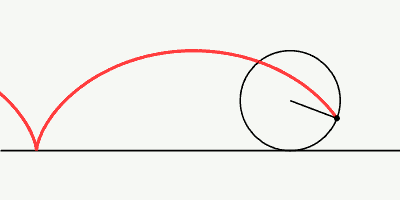
\includegraphics[width=0.3\linewidth]{movies/cycloid/Cycloid_f_static} \textbackslash caption\{The red curve is that traced out by a point on a rolling wheel, by Zorgit \url{https://commons.wikimedia.org/wiki/File:Cycloid_f.gif}\}\label{fig:unnamed-chunk-5}
\textbackslash end\{figure\}

\citet{billHierarchicalStructureEmployed2020} varied the structured motion pattern of the moving discs of an MOT task to show that hierarchical relations are extracted and used to facilitate tracking. The attentional demands, if any, of such hierarchical motion decomposition has not been explored much.

\hypertarget{eyes-to-the-center}{%
\section{Eyes to the center}\label{eyes-to-the-center}}

The human visual system represents scenes as more than just a collection of objects. Our brain's rapid global analysis of visual scenes gives us summary information that is sometimes referred to as ensemble statistics \citep{alvarezSpatialEnsembleStatistics2009}. One such ensemble statistic is the location of the center or centroid of the objects. This is useful for eye movement planning, among other things --- to monitor a group of objects, it is helpful to look at the center of the group, as that can minimize how far into peripheral vision they are situated.

In 2008, \citet{zelinskyEyeMovementAnalysis2008} and \citet{fehdEyeMovementsMultiple2008} independently reported that during multiple object tracking, in addition to gazing directly at targets, the eyes of many participants frequently are directed at blank locations near the center of the array of targets. This basic finding has been replicated by subsequent work \citep{hyonaEyeBehaviorMultiple2019}. The nature of the central point --- whether it is the centroid or something else --- is not entirely clear. Researchers have suggested that it may be the average of the targets' locations, or the average location of all the moving objects (both targets and distractors). Another possibility that has been investigated is that participants tend to look at the centroid of the shape formed by the targets, which recalls the \citet{yantisMultielementVisualTracking1992} hypothesis that what is tracked is the shape defined by the targets. Finally, \citet{lukavskyEyeMovementsRepeated2013} introduced the idea of the ``anti-crowding point'', which is the point that minimizes the ratio between each target's distance from the gaze point and distance from every distractor. The idea was that participants move their gaze closer to a target when it is near a distractor to avoid confusing targets with distractors.

In a comparison of all these metrics against eyetracking data, \citet{lukavskyEyeMovementsRepeated2013} found that the anti-crowding point best predicted participants' gaze in his experiment, followed by the average of the target locations. These points both matched the data better than the centroid of the targets. This undermines somewhat the \citet{yantisMultielementVisualTracking1992} hypothesis that a virtual polygon is tracked, and the finding of best performance by the anti-crowding point is consistent with other results that participants tend to look closer to targets that are near other objects
\citep{vaterDisentanglingVisionAttention2017, zelinskyRoleRescueSaccades2010}.

More work must be done to understand the possible role of an anti-crowding eye movement strategy. Because spatial interference in displays does not seem to extend further than half an object's eccentricity, in both static identification tasks \citep[\citet{gurnseyCrowdingSizeEccentricity2011}]{pelliUncrowdedWindowObject2008} and multiple object tracking \citep{holcombeObjectTrackingAbsence2014}, the anti-crowding point devised by \citet{lukavskyEyeMovementsRepeated2013} ought to be pitted against a measure incorporating the finding that distractors further than about half an object's eccentricity do not cause spatial interference and thus can perhaps be excluded from the calculation.

\hypertarget{whichAspects}{%
\chapter{Which aspect(s) of tracking determine performance?}\label{whichAspects}}

A number of different factors jointly determine how many moving objects we can track and how well we can track them. What are these factors? We've already covered grouping and the nature of the objects themselves, in Chapters \ref{objects} and \ref{grouping}. In this chapter we will briefly outline known factors and how they relate to limited capacity.

Our limited capacity and the reason for it is one of the most important topics in the multiple object tracking literature, as well as attention research more generally. So we'll start off with laying out a framework for thinking about human processing capacities, one that goes beyond the basic bottleneck idea of Chapter \ref{bottlenecks}.

As \citet{normanDatalimitedResourcelimitedProcesses1975} pointed out, the processes that underlie task performance come in two varieties, data-limited and resource-limited. Data in this context means sensory data. If a target moving on an unpredictable trajectory moves outside the edge of our visual field, it is a lack of sensory data that prevents it from being tracked. No amount of mental resources can overcome the absence of any data about an unpredictable stimulus, hence the fact that tracking performance is then limited by the data, or ``data-limited''. This may also be true of cases where sensory signals are impoverished even if not entirely absent. For example, an object traveling at a rate faster than our neurons can register cannot be tracked due to a data limitation. This makes the point that the data being referred to here are not the pattern of light falling on the retina, but rather that light after it has been processed by the retina and after additional preattentive sensory processing.

People with poor visual acuity may perform less well on a task than people with high visual acuity, again due to differences in the sensory data that they have to work with. Thus, some individual differences are almost certainly due to data limitations rather than variation in tracking processes between people. when performance is data-limited, bringing more mental resources to bear may provide little to no benefit. The classic way that this is investigated is by varying the number of stimuli one needs to process. \citet{normanDatalimitedResourcelimitedProcesses1975} illustrate this with a visual search study. If the number of stimuli one must evaluate does not affect how well a person can perform a task, this suggests that the task is data-limited rather than resource-limited, because performance is the same regardless of the proportion of the putative resource can be devoted to it.

When a process is resource-limited, that typically is more interesting for those interested in visual attention and the capacity limits on mental processing. When response time or error rate increases with the number of distractors presented in a visual search task, that was classically interpreted as meaning that a resource-limited process is required for success at the task. As they say, however, science is hard. An elevation in e.g.~error rate will also occur even if there is no resource limitation, but each additional distractor has a non-zero probability of being mistaken for a distractor, then there will be more errors with more distractors even if the probability of successfully evaluating each individual stimulus remains unchanged \citep{palmerAttentionVisualSearch1995}.

The particular number of objects that can be tracked with reasonable accuracy is thus highly dependent on stimulus conditions, and some of these conditions may reflect data limitations rather than a resource limitation. Still, even in ideal conditions it seems clear that the number of objects that can be tracked is much less than the number of objects that are simultaneously processed by early stages of the visual system. There is a resource limitation, and we'd like to know which factors consume the resource. Another way to think of this is with the term that I prefer, ``resource-intensive''. If a deleterious stimulus factor that worsens performance is resource-intensive, this means that increasing the amount of resource devoted the stimulus can compensate for that stimulus factor.

One example is object speed. An increase in object speed can hinder performance, but reducing the number of targets, which provides more resource to the remaining targets, can make up for that. Speed, then, is resource-intensive (although as we will see in chapter \ref{speedAndTime}, there is more going on with speed than most believe). Of course, speed also can result in a data-limitation, at very high speeds, but long before such speeds are reached, speed is resource-intensive.

In summary, to say that tracking is capacity-limited is important, but by itself it is not very illuminating. We want to know more about why people perform more poorly with more targets. Tracking is a complex task, and we would like to know which aspect(s) of it exactly are most capacity-limited.

\hypertarget{unitary-cognition-c1-processes}{%
\section{Unitary cognition (C≈1 processes)}\label{unitary-cognition-c1-processes}}

Tracking may benefit from two resources. One is a resource that can process multiple targets simultaneously, even if it does so more poorly than if there is only one target. A second resource that likely benefits tracking has a capacity of only one target. This reflects a unitary focus of attention that has an approximate capacity of only one. It is the same set of processes that limits us to doing only one 2-digit mental multiplication problem at a time. When applied to tracking, it means you can apply your full intelligence and powers of reasoning to tracking that target, for example to use what you've learned about object trajectories to predict future positions.

The scenario that there are two resources that can benefit tracking makes interpreting the results of experiments complicated. It makes a lot of the results trumpeted by tracking papers uninteresting. Many papers that come out of the experimental psychology tradition (as opposed to psychophysics, which is more quantitative) content themselves with showing that something is true, that a factor matters for performance, p \textless{} .05. Never mind how much it matters, the effect size. This kind of thinking is a real problem across psychology, and in tracking, it leads to me wanting to drag the paper straight into the recycle bin.

As an example, a paper might say that multiple object tracking performance is better with predictable trajectories than with unpredictable trajectories. Well, unless you tell me a lot more, I have to think may be entirely due to our central thought processes that have a capacity of approximately one target. See chapter \ref{beyondLocation} for ways this can be assessed, for now my point is just that this, the possible contribution of C≈1 processes, is something to watch out for.

Another way to put this is that by using our capacity for reasoning and symbol manipulation, we can perform a wide array of arbitrary tasks. We therefore should not be surprised by our ability to track a \emph{single} target. We know that we have a visual system that makes the position and direction of motion of objects on our retina available to cognition, and that using our ability to think about where an object is going and deliberately move our attention to a future anticipated location, we might muddle through tracking a single object.

Even when participants are asked to track several targets, then, one can expect that C=1 processes are contributing to overall performance, even if they are only involved in the processing of one of the targets. Thus, when researchers contrast tracking performance with different numbers of targets, one reason for the decline in performance may be that C≈1 processes are, in each condition, processing only a single target, so performance declines in inverse proportion to the number of targets.

\hypertarget{which-factors}{%
\section{Which factors}\label{which-factors}}

A top priority among tracking reseachers is understanding the reasons that tracking performance falls with the number of targets to track. Does spreading the tracking resource among more targets result in less frequent sampling of each target? More noise in the representation of the spatial location of each target? Poorer predictions of where the targets are going? Fewer neurons devoted to solving the correspondence problem (the correspondence problem will be explained later)? All of the above? Answering these questions would give us very strong clues to how tracking works.

The way forward to answering these questions, and sometimes even the existence of these possibilities, has unfortunately been obscure to many researchers, judging by the literature. Computational modeling is one approach that can be very productive, when done appropriately. Multiple researchers have proposed models, compared their performance on human data, and declared their model a success. Rarely, however, have they compared their model to that of another group of researchers, making it difficult to know whose model is best or whether the data simply doesn't strongly favor one model over another.

Another approach, and the one that I favor, is to start with a task analysis with some conjectures regarding what aspects of MOT trajectories might lead to errors, based on what we know about visual processing, and then manipulate MOT trajectories to test those conjectures. For each aspect that can be linked to errors, once it seems to be isolated (to some degree) by a particular manipulation, one can measure how resource-intensive that aspect's errors are.

Rather than give a chronological account of researchers' halting progress along these lines, I will simply list a few factors that there's now evidence are important, and in the coming chapters explain at greater length what they are, and describe some of the associated evidence.

\begin{enumerate}
\def\labelenumi{\arabic{enumi}.}
\tightlist
\item
  Spatial interference
\item
  Temporal interference
\item
  Object speed
\item
  Use of motion direction
\end{enumerate}

The table below provides an oversimplified summary of what we will learn in some of the following chapters about resource-intensiveness. The degree to which each factor is hemifield specific is also included in the table, because as we will see in Chapter \ref{twoBrains}, knowing that is very important. The literature has not done a good job at determining how resource-intensive some of these factors are, hence some question marks are included in the table.

\begin{table}

\caption{\label{tab:table-limits}Limits on multiple object tracking}
\centering
\begin{tabular}[t]{llll}
\toprule
factor & resource intensiveness & hemifield specificity & contribution to standard MOT\\
\midrule
spatial interference & low? & medium & medium to high\\
temporal interference & high & high? & unknown\\
speed limit & unknown & unknown & low?\\
Use of motion direction & C\textasciitilde{}1 only? & unknown & low\\
\bottomrule
\end{tabular}
\end{table}

By ``contribution to standard MOT'', I mean the degree to which a factor is involved in errors in a task with relatively unconstrained trajectories in the model of Pylyshyn's original work. I have had to make guesstimates for these values due to the lack of relevant work in the literature.

Before going on to address each of these factors, I would also like to address a factor that is somewhat different in kind.

\hypertarget{duration-that-one-can-sustain-attention}{%
\section{Duration that one can sustain attention}\label{duration-that-one-can-sustain-attention}}

Tracking may be, in part, a test of how long one can sustain attention. If a participant gets distracted or starts day-dreaming, that participant might completely stop tracking and, when their attention returns, not know the last locations of the targets. Lapses of attention are a problem in most other laboratory tasks as well, of course, but they are often thought to be particularly important for tracking because tracking requires a longer continuous engagement with the stimuli than for other common laboratory tasks. This is because the trials last for several seconds, typically, and the stimuli are continuously moving, so shifting one's attention away from the display can mean losing the targets.

This greater vulnerability to attentional lapses means that tracking may be more affected by motivation than many other tasks involving visual judgments. Introspectively, it does feel that way to me, relative to many perceptual tasks where I feel I only need to attend for the split-second when the stimuli are presented, and the percept I need to report jumps out at me. The possibility that variability in motivation drives a lot of variability in tracking performance is unfortunate, because we don't study tracking because we're interested in motivation.

It is also possible that the ability to continuously sustain attention may be distinct from general motivation and may cause a lot of variation in tracking. Like motivation, this could hinder efforts to get at the mechanisms specific to tracking that are not simply sustained attention. On the other hand, sustained attention and the limited resource that allows one to track a certain number of targets may be linked. That is, having to track more targets may reduce the amount of time that one can sustain attention on the task. Fortunately, the results of \citet{wolfeMultipleObjectJuggling2007} suggest that this may not be the case.

In Experiment 3 of \citet{wolfeMultipleObjectJuggling2007}, participants were required to track four targets for a period of ten minutes. Every ten seconds or so, one object was highlighted and participants had to indicate whether it was one of the targets. In a no-feedback condition, participants were not told whether their individual responses were correct. In that situation, performance was substantially worse in the last few minutes of the trial than in the first few minutes (78\% correct vs.~65\% correct). However, in the feedback condition wherein participants were told immediately after each judgment whether they were correct, performance did not appear to decline over time. These results suggest that if participants are adequately motivated by feedback, they have considerable ability to track for several minutes with no appreciable loss. The comparison between the feedback and no-feedback conditions is not perfect as the feedback does provide a cue that can increase performance (when participants get the probe wrong, they can increase subsequent performance somewhat by switching to another target), but this confound does not seem to be able to explain the lack of almost any performance loss in the feedback condition.

The circumstances used by \citet{wolfeMultipleObjectJuggling2007} were quite different from a prototypical MOT task, not least because of the extended durations of the trials. Most researchers use trial durations of less than ten seconds, which likely means that a decrease in performance with time due to waning attentino is less of an issue. It seems likely that motivated participants can attend for several seconds before their attention wanes substantially. \citet{oksamaMultipleObjectTracking2004} did find a substantial decrease in performance for trials of 13 s compared to trials of 5 s. With four targets, for example, performance fell from 91\% correct to 74\% correct, and this decrease was somewhat greater for larger numbers of targets than for fewer targets. Byrne \& Holcombe (unpublished data) did not find any significant decrease over a comparable interval, and the explanation for these discrepancies is uncertain, although it may again be related to participants' motivation.

The reason for the reduction in performance with greater time observed by \citet{oksamaMultipleObjectTracking2004} may easily be due to another factor rather than an increase in lapses of attention. In the MOT tasks used by all of these researchers, with longer trials there is likely to be more instances of potential spatial interference, temporal interference, and running afoul of any tracking speed limit. Thus, if any of those factors matter, they could explain the decrease in performance with time. However, the \citet{wolfeMultipleObjectJuggling2007} does seem to provide a kind of existence proof that lapses of attention need not be the limiting factor. Granting that that may be the case, an additional question is why, if other factors are in operation, there was \emph{no} evidence of a performance decrease over time in \citet{wolfeMultipleObjectJuggling2007}? Well, \citet{wolfeMultipleObjectJuggling2007} averaged performance over approximately the first third of the ten-minute interval and compared it to the last third. In the feedback condition, it is possible that all the worst possible events (such as close approaches, causing greater spatial interference) had already occurred by the end of the first third, so whatever level of performance participants were left with at that point already reflected their capacity to track through the most difficult events, which they were then able to continue to do until the end of the trial. Over a shorter time range such as that used by \citet{oksamaMultipleObjectTracking2004}, this may not have been the case.

I know of no studies of what display characteristics make tracking performance more vulnerable to attentional lapses. It stands to reason that if objects are moving very slowly, a lapse may be less detrimental because if after the lapse, one still remembers the last-monitored locations, the targets may still be near them. \citet{fencsikRoleLocationMotion2007} showed that people can reacquire targets after a 300 millisecond disappearance, and \citet{alvarezMultielementVisualTracking2005} showed that people can do this after being interrupted by a second task, although these interruptions are obviously different than an attentional lapse, during which it's not clear how often people forget the target locations.

Vigilance tasks such as the gradual-onset continual performance task are expressly designed to assess sustained attention and lapses over an extended interval, and an individual-differences study by \citet{trevinoBridgingCognitiveNeuropsychological2021} found that MOT performance had little correlation with a five-minute gradual-onset continual performance task. This is somewhat reassuring as it, like some of the other evidence I have mentioned, suggests that lapses are not a major determinant of MOT performance.

\hypertarget{spatialInterference}{%
\chapter{Spatial interference}\label{spatialInterference}}

Details of the world that are much smaller than ourselves, like the fibers of a piece of paper, or the individual blotches laid down on paper by a printer, are inaccessible to the naked eye, largely because our photoreceptors are too widely-spaced. This is a familiar limit on our visual abilities, one that is measured every time we go to the optometrist. Line segments or objects that are too close together are experienced is a single unit.

Critically, even when two objects are spaced far apart enough that they can easily be seen to be two objects rather than one, they are not processed entirely separately by the brain. Receptive fields grow larger and larger as visual signals ascend the visual hierarchy, and this can result in a degraded representation in the visual system for objects that are near each other. In other words, spatial interference ensues.

A large body of psychophysical work has investigated the display densities that impair object perception. Common tasks in this literature include letter identification and grating orientation discrimination \citep[e.g.,][]{wolfordPerturbationModelLetter1975, korteUberGestaltauffassungIm1923, strasburgerDancingLettersTicks2014}.

\begin{figure}
\centering
\includegraphics{tracking-review_files/figure-latex/unnamed-chunk-6-1.pdf}
\caption{\label{fig:unnamed-chunk-6}When one gazes at the central dot, the central letter to the left is not crowded, but the central letter to the right is.}
\end{figure}

In the above display, if you gaze at the central dot, you likely will be able to perceive the middle letter to the left fairly easily as a `J'. However, if while keeping your eyes fixed on the central dot you instead try to perceive the central letter to the right, the task is much more difficult. This spatial interference phenomenon is called ``crowding'' in the perception literature.

Most studies of crowding ask participants to identify a target such as a letter when flanking stimuli are placed at various separations from the target. The separation needed to avoid crowding varies depending on the display spatial arrangement, but on average is about half the eccentricity of the target; the interference diminishes rapidly as separation increases beyond that \citep{boumaInteractionEffectsParafoveal1970a, gurnseyCrowdingSizeEccentricity2011}. In the display above, for example, the letters on the same side as the `J' are separated from it by more than half the 'J's distance from the fixation point, so they have little to no effect on its identification.

When flankers are presented close to a target, they not only prevent identification of the target, they can also prevent the target from being individually selected by attention, which likely spells trouble for multiple object tracking \citep{intriligatorSpatialResolutionVisual2001}. When a target and distractor are too close to be distinguished by tracking processes, the tracking process may inadvertently end up tracking a distractor rather than the target.

Crowding happens frequently in typical MOT displays, in that in most experiments, objects are not prevented from coming within half the eccentricity of each other. It is not surprising, then, that in typical MOT displays,
greater proximity of targets and distractors is associated with poor performance \citep{shimSpatialSeparationTargets2008, tombuAttentionalCostsMultipleobject2008}.

\hypertarget{spatial-interference-does-not-explain-why-tracking-many-targets-is-more-difficult-than-tracking-only-a-few}{%
\section{Spatial interference does not explain why tracking many targets is more difficult than tracking only a few}\label{spatial-interference-does-not-explain-why-tracking-many-targets-is-more-difficult-than-tracking-only-a-few}}

\citet{franconeriTrackingMultipleObjects2010a} claimed that spatial interference is the \emph{only} reason why performance is worse when more targets are to be tracked, denying any role for speed, time, or a resource that is depleted when more targets must be tracked. They posited that tracking errors, other than lapses of concentration, are caused entirely by the poor spatial resolution of tracking's selection process, together with inhibitory surrounds that can cause mutual interference among the selection of nearby targets. The most provocative tenet of their theory was that ``there is no limit on the number of trackers, and no limit per se on tracking capacity'' (p.920), implying that a very large number of targets could be tracked if they were kept far apart from each other.

In pursuing tests of this theory, \citet{franconeriTrackingMultipleObjects2010a} unfortunately did not isolate the separation between objects from other display variables. More generally in the literature, MOT studies rarely control the retinal separation among the objects in a display. For example, \citet{franconeriTrackingMultipleObjects2010a} kept object trajectories essentially constant in their experiments but varied the total distance traveled by the objects (by varying both speed and trial length), on the basis that if close encounters were the only cause of errors, they should be proportional to the total distance traveled. When they found that performance did decrease with distance traveled, but there was little effect of the different object speeds and trial durations that they used, they took this as strong support for their theory that only spatial proximity mattered.

As \citet{franconeriTrackingMultipleObjects2010a} wrote in their conclusion, their hypothesis that ``barring object-spacing constraints, people could reliably track an unlimited number of objects as fast as they could track a single object'' constituted a ``simple and falsifiable hypothesis''. I believed this hypothesis to be unlikely to be true, and on obvious test was to keep all the objects in an MOT display widely separated, vary the number of targets, and measure the speed threshold in each case.

In 2012, my student Wei-Ying Chen and I conducted several experiments in this vein. In one, we used an ordinary computer screen but had participants bring their noses quite close to it to create a wide-field display, which allowed us to keep targets and distractors dozens of degrees of visual angle from each other \citet{holcombeExhaustingAttentionalTracking2012}. The basic display configuration is shown below .

\begin{figure}
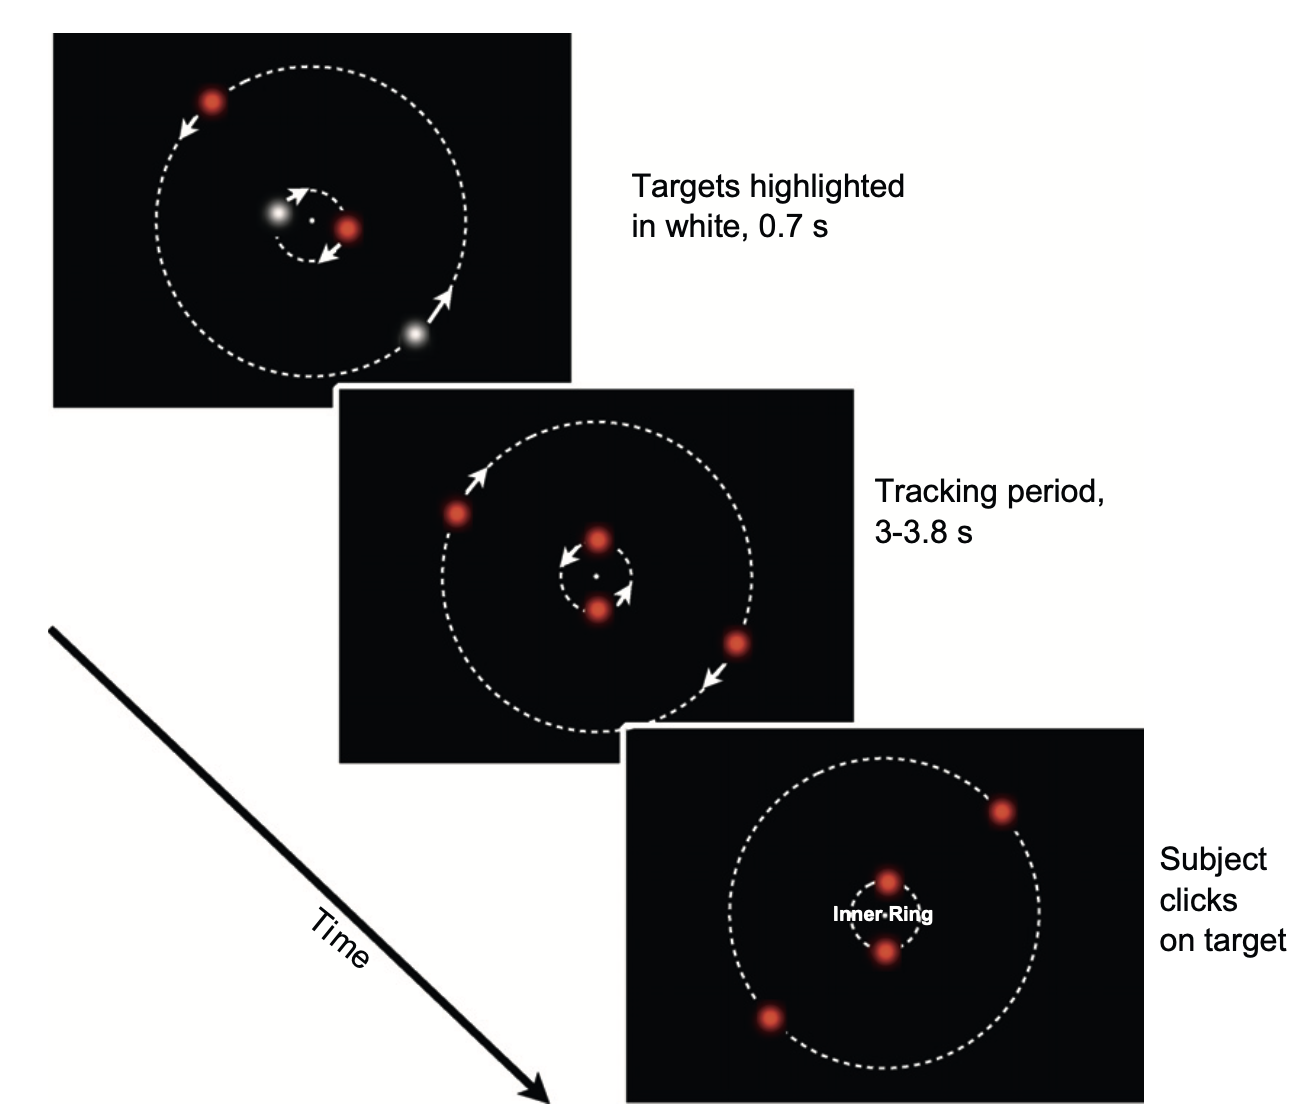
\includegraphics[width=1\linewidth]{imagesForRmd/HolcombeChen2012BasicTrial} \caption{In experiments by Holcombe & Chen (2012), after the targets were highlighted in white, all the discs became red and revolved about the fixation point. During this interval, each pair of discs occasionally reversed their direction. After 3–3.8 s the discs stop, one ring is indicated by presenting text next to it, and the participant clicks on one disc of that ring.}\label{fig:HC2012BasicTrial}
\end{figure}

We found that even with objects extremely widely-spaced speed thresholds declined dramatically with the number of targets. To us, this appeared to falsify the theory of \citet{franconeriTrackingMultipleObjects2010a}. Indeed, for the 2011 Vision Sciences Society conference where we reported these findings, we entitled our poster entitled ``The resource theory of tracking is right! - at high speeds one may only be able to track a single target (even if no crowding occurs''. What we meant was that each target takes up some of a very limited processing capacity - a resource that was attentional in that it could be applied anywhere in the visual field, or at least anywhere within a hemifield (\ref{twoBrains}). The amount of this resource applied to a target determines the fastest speed at which a target can be tracked.

Franconeri, together with his colleagues George Alvarez and Patrick Cavanagh (of whom the latter was, incidentally, my PhD advisor) were not convinced by the findings of Wei-Ying Chen and I. Franconeri et al.~not only continued to push their spatial interference theory of tracking, but also they suggested the same basic idea could explain capacity limits on object recognition, visual working memory, and motor control, writing that ``competitive interactions are the roots of capacity limits for tasks such as object recognition and multiple object tracking'' (p.2) and that capacity limits arise only because ``items interact destructively when they are close enough for their activity profiles to overlap'' (p.2) \citet{franconeriFlexibleCognitiveResources2013}. Yet to explain the \citet{holcombeExhaustingAttentionalTracking2012} results, the spatial interference posited by Franconeri would have to extend over a very long distance, farther than anything that had been reported in behavioral studies. Furthermore, if there were such long-range spatial gradients of interference present, they should have shown up in the results of \citet{holcombeExhaustingAttentionalTracking2012} as worse performance for the intermediate spatial separations we tested than for the largest separations we tested.

To address these issues with their theory, \citet{franconeriResourceTheoryNot2013} appealed to data from recordings in the lateral intraparietal area (LIP) of rhesus macaque monkeys. In a study by \citet{falknerSurroundSuppressionSharpens2010}, the monkeys were presented with a saccade target, and the monkey was cued to execute a saccade to it by offset of the fixation point. In some trials, however, another stimulus was flashed 50 ms prior to the offset of the fixation point. That flashed stimulus was positioned in the receptive field of an LIP cell the researchers were recorded from, and it was found that its response was suppressed relative to trials when there was not a saccade target. This was true even when the saccade target was very far away, with statistically significant impairment at separations up to 40 deg for some cells. There was a spatial gradient, but the data suggested it could be quite shallow, allowing \citet{franconeriResourceTheoryNot2013} to write that ``levels of surround suppression are strong at both distances, and thus no difference in performance is expected'' for the separations tested by Holcombe and Chen (2012). Note that \citet{franconeriResourceTheoryNot2013} was published as an online comment at \emph{Trends in Cognitive Sciences}, as a reply to my online comment pointing out some of the problems with their theory. Unfortunately, some time later, probably in 2018, both comments were lost by the publisher, Elsevier, when they migrated their system. In the case of my comment, however, I found an old version on my computer, updated it slightly and posted it at \citet{holcombeCommentCapacityLimits2019}.

One property of the neural suppression documented by \citet{falknerSurroundSuppressionSharpens2010} strongly suggests it is not one of the processes that limit our ability to track multiple objects. Specifically, \citet{falknerSurroundSuppressionSharpens2010} found that nearly as often as not, the location in the visual field that yielded the most suppression was not in the same hemifield as the receptive field center. But as we will see in \ref{twoBrains} the cost of additional targets in attentional tracking is largely independent in the two hemifields, suggesting that LIP suppression is not the main factor yielding worse performance when there are more targets. Instead, as \citet{falknerSurroundSuppressionSharpens2010} themselves concluded, these LIP cells may help mediate a global salience computation for prioritizing saccade or attentional targets wherever they are in the visual field.

In light of all the above, it seemed the evidence ruled against the idea that spatial interference was the sole reason that people perform worse with more targets. By 2013, the spatial interference account advocated by Franconeri seemed to have been watered down until it was practically indistinguishable from a resource theory. That is, if spatial interference extended over an entire visual field (or hemifield) with no detectable diminution at large separations relative to small separations, then it no longer seemed appropriate to refer to it as ``spatial'' interference. Instead, finite processing capacity seems to be both a more parsimonious and straightforward description.

The word ``resource'' appropriately conveys that people can choose how to apply their finite processing capacity, as a resource is something that is available to someone and can be used in different ways. For example, it suggests that one can use half of one's processing capacity for one target while using the other half for a second target. The validity of this part of the metaphor is addressed by some experimental evidence reviewed in \ref{twoBrains} and \ref{serialOrParallel}.

Having failed to find evidence for long-range spatial interference, I decided to investigate the form of spatial interference that I was confident actually existed: short-range interference. As mentioned in the first section of this chapter, we were already confident that short-range spatial interference existed, from some previous studies of tracking. However, these studies did not provide much evidence about how far that interference extended - either they did not control eccentricity (e.g. \citet{feriaSpeedHasEffect2013}) or they only tested a few separations (e.g. \citet{tombuTrackingPlanetsMoons2011}).

In experiments published in 2014, we assessed tracking performance for two targets for various separations between the targets' trajectories \citep{holcombeObjectTrackingAbsence2014}. Performance improved with separation, but only up to a distance of about half the target's eccentricity, similar to what has typically been found in the crowding literature \citep{strasburgerDancingLettersTicks2014}. In a few experiments there was a trend for better performance even as separation increased beyond the crowding zone, but this effect was small and not statistically significant. In all experiments performance was substantially worse for large separations, even for the largest separation tested of 59 degrees of visual angle. These findings supported my suspicion that spatial interference is largely confined to the crowding range, and that the performance deficit when there are more targets to track is caused by a limited processing resource.

The experiments we reported in \citet{holcombeObjectTrackingAbsence2014} did yield one surprise. In the one-target conditions, outside the crowding range we found that performance actually decreased with separation from the other pair of (untracked) objects. This unexpected cost of separation was only statistically significant in one experiment, but the trend was present in all four experiments that varied separation outside the crowding range. This might potentially be explained by the configural or group-based processing that I reviewed in \ref{grouping}, as grouping of distant elements tends to occur less often than for nearby elements \citep[e.g.,][]{kubovyLawfulnessGroupingProximity1998}.

What is the nature of the short-range spatial interference that we and others have documented? As explained in the beginning of this chapter, one cause of spatial interference is simply lack of spatial resolution by the processes that mediate tracking. If a process cannot distinguish between two locations, either because of a noisy representation of those locations or because the two locations are treated as one, then a target may often be lost when it comes too close to a distractor. This would be true of any imperfect mechanism, regardless of whether it is biological or man-made.

While some form of spatial interference or confusion is well-nigh universal, the particular way that the human visual system is put together may result in forms of spatial interference that do not occur in, for example, computer algorithms engineered for object tracking. As described in \ref{bottlenecks}, our visual processing architecture has a pyramid-like structure, with processing at the retina being local and massively parallel, and then gradually converging such that neurons at higher stages have receptive fields responsive to large regions. At these higher stages processes critical to tasks like tracking or face recognition occur. Face-selective neurons, for example, are situated in temporal cortex and have very large receptive fields. For tracking, while the parietal cortex is thought to be more important than the temporal cortex, the neurons in these parietal areas again have large receptive fields.

A large receptive field presents a problem when the task is to recognize an object in clutter or to track a moving target in the presence of nearby moving distractors. In the case of object recognition, without a mechanism to prevent processing of the other objects that share the receptive field, object recognition would have access to only a mishmash of the objects' features. Indeed, this indiscriminate combining of features is thought to be one reason for perceptual illusory conjunctions. Similarly, for object tracking, isolating the target is necessary to keep it distinguished from the distractors.

In principle, our visual systems might include attentional processes that when selecting a target can completely exclude distractors' visual signals from reaching the larger receptive fields. Actually implementing such a system using realistic biological mechanisms with our pyramid architecture, however, looks to be difficult \citep{tsotsosModelingVisualAttention1995}. Neural recordings reveal that while the signals from stimuli irrelevant to the current task are suppressed somewhat, they still affect neural responses. The particular mechanism used by our visual system appears to include active suppression of a region around a target, which has long been championed by the computer scientist John Tsotsos as a practical way for high-level areas of the brain to isolate a stimulus in their large receptive fields. This suppression likely involves descending connections from high-level areas and possibly recurrent processing \citep{tsotsosDifferentStagesVisual2008}.

Note that on this account, it is only targets, not distractors, that have a region of suppression surrounding them. One consequence of this is that when one tracks more than one target, there is the potential for the targets to suppress each other's selection process. Indeed, this was one basis of the contention of \citet{franconeriTrackingMultipleObjects2010a} that the limit on number of targets that can be tracked was caused entirely by spatial interference. While their attempt to attribute all of the cost of tracking additional targets to surround suppression may be misguided, in \citet{holcombeObjectTrackingAbsence2014} we did find some tentative evidence supporting a greater range of interference in the two-target condition compared to the one-target condition. Again, the effect was small relative to the total additional-target performance cost. It appears that overlapping surround suppression associated with targets may impair tracking, but the spatial range of this does not extend much beyond the classic crowding range.

Crowding, or the impairment of object identification by nearby objects, has generally been studied more extensively than the spatial interference associated with object tracking. Like for tracking, however, the possibility of suppression around targets remains understudied. Very few studies of crowding have varied the number of targets. I have found one study of the identification of briefly-presented stimuli which found that attending to additional gratings within the crowding range of a first grating resulted in greater impairment in the letter identification task \citep{mareschalAttentionalModulationCrowding2010}. This is consistent with the existence of surround suppression around each target.

In summary, spatial interference likely contributes to many errors in tracking when targets and distractors come close to each other. This may be mediated partly by surround suppression around targets, as well as the inherent ambiguity regarding which is a target and which is a distractor during close encounters for a limited spatial resolution system. When objects are kept widely separated, it appears that spatial interference plays little to no role in tracking. Some other factor or factors, such as some sort of attentional resource, is needed to explain the dramatic decline in tracking performance that can be found with more targets even in widely-spaced displays \citep{holcombeObjectTrackingAbsence2014, holcombeExhaustingAttentionalTracking2012, holcombeSplittingAttentionReduces2013}.

\hypertarget{beyondLocation}{%
\chapter{The role of motion}\label{beyondLocation}}

Motion is obviously part and parcel of multiple object tracking. The visual system of animals such as humans have specialized motion processors that are not driven by arbitrary signals of an object's displacement, rather they have particular signals associated with motion that they are especially responsive to \citep{nishidaAdvancementMotionPsychophysics2011}. These signals can be selectively disrupted, while preserving the physical displacment of the objects. \citet{clairConflictingMotionInformation2010} did this in an MOT paradigm by having the texture elements that patterned the moving objects move in a different direction than the objects themselves. Tracking was still possible, but was disrupted quite a lot. This suggests that tracking is driven by the specialized motion detectors, which likely help carry along a selection focus of tracking as a target moves. This is further supported by studies involving large jumps between successive appearances of a moving target, also known as ``apparent motion'', which find lower temporal limits on tracking for these stimuli (the notion of temporal limits will be explained in chapter \ref{speedAndTime}) \citep{kanayaContributionNonattentiveMotion2012, verstratenLimitsAttentiveTracking2000}.

It does not seem controversial that motion processing is somewhat distinct from the tracking resource, and that it is used by tracking. A more open question is whether motion signals are used in two particular ways. One is whether the direction and speed of a target is used to anticipate future positions of the objects, then performance should be better when objects maintain straight-line trajectories than when they frequently change their direction.

The evidence below suggests that the capacity limit on the use of motion information during tracking may be more severe than that on the use of position. That is, in conditions where participants can use position information to accurately track four or five targets, they may only use motion information for one or two of the targets. This may mean that the use of motion information can be identified with the extended cognitive processing of an object that likely can only occur for one or at most a few targets, which was referred to in Chapter \ref{whichAspects} as C≈1 processes.

\citet{howeMotionInformationSometimes2012} compared a condition in which the objects moved in straight lines, only changing direction when they bounced off the arena's boundaries, to when the objects' trajectories were not predictable because they changed direction randomly about every half second. However, this advantage for tracking the predictable trajectories was found when there were two targets, but not when there were four targets. \citet{vulExplainingHumanMultiple2010} asked participants to track three targets and varied how much and how often the objects changed their velocity. They found little to no detriment of the velocity changes on participants' estimates of difficulty. Unfortunately they did not assess whether velocity continuity became beneficial with fewer targets.

In the \citet{howeMotionInformationSometimes2012} experiments, participants were allowed to move their eyes. They may have moved their eyes to follow one target, or alternatively something like the centroid of the targets (see \ref{grouping}), and as eye movements have some associated inertia, that tendency to continue moving the eyes in the same direction might have contributed to the predictable trajectory benefit, and it makes sense that this would boost conditions with fewer targets more given that the eyes only move in one direction at a time. \citet{luuExtrapolationOccursMultiple2015} followed up on the \citet{howeMotionInformationSometimes2012} results using similar experiment parameters but added a requirement that participants fixate at the center of the screen throughout a trial, and found a very similar pattern of results.

These results converge nicely with those of \citet{fencsikRoleLocationMotion2007}, who made targets invisible for a brief period (307 ms) during tracking. The targets continued moving, invisibly, during the disappearance interval, and participants were able to continue tracking afterward when there were one or two targets but not four targets, as evidenced by better performance compared to a control condition where prior motion information was not available.

\citet{wangRoleKinematicProperties2021} devised displays that allowed them to compare the extent to which participants used position information, velocity, and acceleration during tracking. Consistent with previous investigations, velocity was used less than position, and was subject to a more severe capacity limit. Acceleration (extrapolation of change in motion direction) did not seem to be used at all.

\hypertarget{velocity-as-a-feature-for-correspondence-matching}{%
\section{Velocity as a feature for correspondence matching?}\label{velocity-as-a-feature-for-correspondence-matching}}

For tracking, motion information could be used in two different ways. One is to solve what is referred to as the ``correspondence problem''. To understand this, imagine that the moving objects in an MOT display were sampled by a computer only once every three hundred milliseconds (something like this may be what the brain does when there are several targets, if attention samples objects serially - \ref{serialOrParallel}). The correspondence problem is to determine the correspondence between the objects of the two frames. That is, solving the correspondence problem means knowing where an object in the first frame is in the second frame. The rise of CCTV a few decades ago sparked a rapid growth in the development of algorithms for tracking objects in low frame rate video \citep{kamkarMultipletargetTrackingHuman2020}. The correct answers for which objects in frames 1 and 2 correspond to each other can in many situations be obtained by nearest-neighbor matching. Nearest-neighbor here simply means matching each object in frame 1 to that closest to it in frame 2.

For some combinations of object trajectories and sampling frequencies, the nearest-neighbor match yields the wrong answer to the correspondence problem. For example, if in the interval between the two sampled frames, a distractor moving toward the target ends up very close to a target's location in frame 1, while the target has moved farther from its frame 1 location, then using nearest0neighbor will mistakenly match the target in frame 1 with a distractor in frame 2. This is called a ``false correspondence''.

Using nearest-velocity matching in conjunction can help avoid false correspondences. Velocity refers to both an object's direction and its speed. Because moving objects maintain their current velocity for a few hundred milliseconds or more, depending on the display, when two objects in frame 2 are both very close to the location a target occupied in frame 1, the target is likely to be the object whose velocity is most similar to the velocity of the target in frame 1. This topic will be discussed more in Chapter \ref{resolution}, because it relates to the motion streaks idea of that chapter..

\hypertarget{velocity-for-position-estimation}{%
\section{Velocity for position estimation}\label{velocity-for-position-estimation}}

The use of velocity matching to solve the correspondence problem must be distinguished from the topic of this section, using velocity to estimate position. A velocity signal can be used to predict or extrapolate the next position of a moving object. Consider a discrete sampling situation where one has a set of sensory signals of object locations on frames 1, 2, and 3. One can use the velocity signal for a target at frame 2 to extrapolate where it should be on frame 3. Then, when the sensory signals for frame 3 arrives, one can use the extrapolated target position as the input for solving the correspondence problem rather than the frame 2 position. I call this extrapolation of the present because if the brain uses this scheme, the idea is not that a person would perceive a moving object in a potential future position. Instead, the process is one of using the trajectory a target was on to help determine which new sensory signal corresponds to it.

The experiments reviewed in the first section of this chapter found evidence for the use of motion information, but that type of evidence could not distinguish between the use of motion for extrapolating the present and the use of motion for velocity matching. As we will see next, the results from two other paradigms find little to no evidence of extrapolation, which suggests that velocity matching is the way that motion information is used.

The first paradigm that was used to go looking for evidence of extrapolation, the ``target recovery'' paradigm, was developed by \citet{keaneMotionExtrapolationEmployed2006}. They had objects abruptly disappear during MOT and then reappear hundreds of milliseconds later. In their ``move'' conditions, they re-appeared further along the trajectory they would take had they continued with the same velocity, whereas in ``non-move'' conditions they would reappear in the same position they had disappeared in. Performance was uniformly worse in the move conditions than in the non-move conditions. A follow-up study by \citet{franconeriSimpleProximityHeuristic2012} found the same result.

The possibility of extrapolation has also been explored by simply asking participants to report the last location of a target or targets after they disappear, by clicking with a mouse on the screen. If the brain extrapolates the present, that should result in participants reporting, on average, the correct last position of the target, although individual reports might be quite noisy. The brain might alternatively extrapolate the future, as has often been suggested (e.g. \citet{nijhawanVisualPredictionPsychophysics2008}), such that on average participants would click on a position ahead of a target's last position. Instead, studies have predominantly found that the locations participants report lag the final locations of the target, and this lag increases with the number of targets tracked \citep{howardTrackingChangingFeatures2008, howardPositionRepresentationsLag2011}. One exception is from \citet{iordanescuDemandbasedDynamicDistribution2009}, who found that people clicked on average slightly ahead of the target's last position. However, \citet{howardPositionRepresentationsLag2011} tried but failed to replicate this result, instead finding lags again.

Further evidence that the visual system uses a lagged representation comes from an MOT eye-tracking study by \citet{lukavskyGazePositionLagging2016}. They were able to assess whether eye position either anticipated future positions of the objects or instead lagged their present position in an ingenious model-free way. They contrasted the eye movements in pairs of trials with object paths that were identical except that their trajectories were time-reversed. After reversing the timeline of the eye movement data from the backward trials, they time-shifted that data to find the time shift that maximized the correspondence of the eye movements for the two kinds of trials. In their first and second experiment, with four targets, the time-shifting technique of \citet{lukavskyGazePositionLagging2016} revealed that eye movements lagged the targets in every participant, with a mean lag of 110 ms in the first experiment and 108 ms in the second experiment.

Recall that a promising theory of tracking is that a process switches among the targets to update their positions - this would explain the dramatic worsening of temporal limits with additional targets reviewed in \ref{speedAndTime}. such a theory also entails that not only temporal limits, but also lags should worsen with additional targets. This is precisely what was found by \citet{howardTrackingChangingFeatures2008} varied the number of targets from one to seven and found that the lag of the positions participants clicked on increased with the number of targets tracked. This supports a serial position sampling theory, as discussed in \ref{serialOrParallel}. A trend but \emph{not} a statistically significant increase, however, was found by \citet{howardPositionRepresentationsLag2011}; they only varied the number of targets from one to three, and perhaps that was not enough. \citet{lukavskyGazePositionLagging2016} also investigated whether the lag changed with the number of targets, in their case the lag of eye position. In their second experiment numerically the mean lag was 15 ms less (93 ms) for two targets than for four, although again this was not a statistically significant difference - the 95\% confidence interval spanned from 33 ms of lag to 2 ms of extrapolation. Thus while their results were compatible with the proposition that there is less lag with fewer targets, the data did not strongly support it. More work should be done in this area.

\hypertarget{simulation-evidence-indicates-that-extrapolation-has-little-value-in-mot}{%
\section{Simulation evidence indicates that extrapolation has little value in MOT}\label{simulation-evidence-indicates-that-extrapolation-has-little-value-in-mot}}

The evidence of the preceding sections suggests that tracking processes do little in the way of extrapolation, or even velocity matching, except for when there are only a few targets, when more limited-capacity cognitive processes may play a larger role. The paucity of evidence for extrapolation is surprising in light of the popularity of predictive frameworks for conceptualizing what the brain does. Many researchers believe that prediction is a critical component of much of perception. So, is the brain leaving a lot of performance gains on the table by not using extrapolation when there are more than a few targets?

A computational investigation by \citet{zhongWhyPeopleAppear2014} found that there is little to be gained by extrapolation in standard MOT tasks. \citet{zhongWhyPeopleAppear2014} took an approach resembling what is often called an ``ideal observer'' approach. The idea is to build into a model the relevant properties of our sensory limitations and then assess how well an optimal algorithm for processing those signals would do, and investigate how it would be affected by task parameters. \citet{zhongWhyPeopleAppear2014} did this by turning a Kalman filter loose on estimating object positions for use to solve the correspondence problem in MOT. In the term ``Kalman filter'', the word ``filter'' has a tendency to mislead people, as it is not a filter in the conventional sense. The Kalman filter is instead an algorithm that learns to estimate, in Bayesian fashion, the current position of the targets. Bayesian estimation is appropriate because the sensory estimates of the objects are not precise - the simulations of \citet{zhongWhyPeopleAppear2014} assume that the sensory error is Gaussian-distributed, which is a reasonable approximation, although \citet{zhongWhyPeopleAppear2014} also make various simplifying assumptions, such as that the Gaussian error has the same variance throughout the visual field.

The Kalman filter makes a prediction of the object's current position, based on its best estimate of the object's last position and its velocity. This prediction, based on previous sensory position signals and a velocity estimated from them, is combined with the current sensory position signal to yield the estimate of the object's current position. The relative weights assigned to the prediction and the sensory signal are determined by an updating process that arrives at the optimal weights under certain assumptions.

\citet{zhongWhyPeopleAppear2014} took the position estimates of the targets provided by the Kalman filter on each time step and used them to solve the correspondence problem. That is, rather than matching the sensory position data of the current frame to each sensory position datum from the previous frame believed to have been from a target, instead of this sensory data from the previous frame, they used the Kalman filter estimates of each target's position. \citet{zhongWhyPeopleAppear2014} expected that simulated MOT task accuracy would be substantially higher when the Kalman filter was used, because the Kalman filter estimates of each target's position are substantially more accurate than the `raw' sensory data.

To the surprise of the researchers, simulated MOT performance was not substantially higher for the Kalman filter than when the raw sensory data was used. This finding was robust to a range of parameter values for the simulation, so \citet{zhongWhyPeopleAppear2014} concluded that extrapolation has very little benefit for the MOT tasks they investigated.

To understand this result, \citet{zhongWhyPeopleAppear2014} suggested that one must first consider the situations that lead to errors in MOT. As we have suggested elsewhere in this book, most errors may arise during close encounters between targets and distractors. During the periods of an MOT trial when the targets and distractors are far from each other, there is no correspondence ambiguity and computational models such as that of \citet{zhongWhyPeopleAppear2014} do not make mistakes, so extrapolation and velocity matching are certainly of no benefit there. During close encounters, by contrast, one might expect that extrapolation would reduce false correspondences. In their simulations, \citet{zhongWhyPeopleAppear2014} found that extrapolation did reduce false correspondences, improving task performance but that this benefit was extremely small in size.

Why is there only a trivial benefit of extrapolation in the \citet{zhongWhyPeopleAppear2014} simulations? False correspondences in the simulations are caused by noise in the incoming sensory position signals. The Kalman filter's representation is less noisy than the sensory signals, in part due to extrapolation, but the improvement in accuracy is dwarfed by the sensory noise, as far as resulting false correspondences. In other words, targets end up being swapped for distractors (false correspondence) largely due to the ambiguity in correspondence created by the sensory noise. This remained true for each of the different levels of sensory noise and intermittency of sampling that \citet{zhongWhyPeopleAppear2014} simulated.

More work needs to be done with this sort of approach. \citet{zhongWhyPeopleAppear2014} made some assumptions that are known to be false, such as that there is a uniform level of sensory noise across the visual field, and some that are implausible, such as that the brain can determine a global solution for the correspondence problem that minimizes the sum of the distances between the targets' position estimates provided by the Kalman filter and the new sensory observations. At least some of their results are probably robust to these assumptions, but possibly not all.

\hypertarget{a-c1-extrapolation-effect}{%
\section{A C≈1 extrapolation effect?}\label{a-c1-extrapolation-effect}}

Another behavioral paradigm in which participants report the last position of an object does frequently elicit evidence of extrapolation. In this ``representational momentum'' paradigm, participants are typically shown only a single moving object and asked to report the object's final position after it suddenly disappears. On average, participants usually indicate a position displaced in the object's final direction of motion. \citet{hubbardRepresentationalMomentumRelated2005} provides an extensive review of a large literature on this. Participants were also found to displace the last position of a target in the direction of gravity. The phenomenon may reflect C=1 cognitive processes, but this remains uncertain because the number of objects is almost never varied in this literature.

Another extrapolation phenomenon has been reported for frozen-action photographs that imply motion. For example, \citet{freydMentalRepresentationMovement1983} presented a photograph such as of waves crashing on a beach, and participants judged whether a subsequently presented probe photograph was the same as the original photograph or different. The pattern of response time suggested that participants' memory of the photograph was closer to one from later in the series of photographs than the original. \citet{hafriMeltingIceYour2022} found that this form of extrapolation generalized to changes in state that could not easily be reduced to motion. For example, they found that an image of a burning log was remembered as being more burnt than it was in the original photograph.

In the literature, the term ``representational momentum'' is applied to both the extrapolations of the state of a stimulus like a burning log and the reported position of a moving object whose trajectory is abruptly terminated, although I don't know of strong evidence that these reflect the same phenomenon. However, it is plausible that these reflect a C≈1 process and thus would not show hallmarks of MOT such as hemifield independence. Because this sort of likely-cognitive or memorial process exists, researchers who are interested in the processes that underlie tracking should assess whether their findings can be explained by C≈1 processes before assuming that what they are studying is perceptual or attentional rather than cognitive. This issue is discussed further in the Recommendations section.

It is also possible that representational momentum is a memory effect, perhaps reflecting the same mechanisms that yield the boundary extension effect discovered by Helene Intraub \citep{intraubBoundaryExtensionFundamental1993}. However, \citet{nakayamaDynamicNoiseBackground2021} recently discovered an extrapolation effect that appears to be perceptual, in that this ``twinkle goes'' illusion shows up with immediate report and is immediately perceived by many observers \href{https://twitter.com/ceptional/status/1204116417429131264}{in demonstrations}. The results from one experiment investigating this effect suggest that it is highly resource-intensive, however, because when attention was split across two targets the effect was greatly diminished. Possibly, then, the twinkle-goes illusion reflects a C≈1 effect, although more work is needed.

In summary then, there is little evidence for extrapolation playing a role in multiple object tracking, with the possible exception of a C≈1 effect for one of the targets, if it is particularly attended to.

\hypertarget{speedAndTime}{%
\chapter{Speed limits and temporal limits}\label{speedAndTime}}

Naturally there are speeds at which moving objects cannot be tracked. If we had a particular sort of brain, we'd be able to track any object whose motion we could perceive. But animal brains like ours provide for the perception of motion with a system that is quite independent of the processes that allow for tracking.

Motion direction is sensed by direction-selective cells that are arrayed in retinotopic cortex such that there are cells that respond fairly independently to motion in each part of the visual field. The responses of these cells, as they feed into higher motion-processing areas such as MT/MST, eventually give rise to the experience of motion, even though this does not seem to involve tracking. That is, these cells do not know where the object they are responding to has been previously, they are basically motion sensors that respond when there is motion of a particular direction in their receptive field.

Tracking implies the existence of some index or pointer that represents that a particular object is the same as one of the set of objects designated as targets at the beginning of the trial. Even when there is only one target, this process falters at far lower speeds than perception of the target's motion \citep{verstratenLimitsAttentiveTracking2000}. Moreover, the maximum speed at which one can track is lower when there are more targets \citep{holcombeExhaustingAttentionalTracking2012}. What is it about the tracking process that gives it these properties?

An increase in object speed will have multiple consequences in a typical MOT experiment. In a standard MOT display, as the targets and distractors wander around the screen, they occasionally come very close to each other (in some experiments, they touch each other or even pass through each other). As discussed in section \ref{spatialInterference}, very close encounters can result in the loss of a target. That is relevant to the issue of speed because when MOT researchers vary object speed, they typically keep trial duration constant, so that the objects travel farther during the higher-speed trials. As a result, the objects have more close encounters, so the reason for poorer performance could simply be due to that.

A first step to revealing the effect of speed, then, is to assess it without the contaminating effect of an increase in close passes. \citet{holcombeExhaustingAttentionalTracking2012} did this by by keeping the objects very far from each other as well as
using shorter trials for fast speeds, so that objects traveled the same total distance for different speeds, just in case there were any long-distance spatial interactions. The speed thresholds that resulted were still far below those for motion perception, suggesting that speed has a deleterious effect on tracking even without any concomitant close encounters, and in a range where the simple perception of motion is yet to be affected. Moreover, participants' speed thresholds were much lower when two targets had to be tracked compared to when just one target was tracked. One way to refer to this is to say that speed consumes the tracking resource.

It is tempting to conclude that devoting more tracking resource to a target results in the associated internal pointer being able to move faster across the retina. This conclusion would be premature. There remains another possible reason that tracking falters at high speeds.

\hypertarget{a-temporal-limit-on-perception}{%
\section{A temporal limit on perception}\label{a-temporal-limit-on-perception}}

When two objects appear in a common location very close in time, they will be combined by the visual system. If one flickers a light off and on at a very rapid rate (about 60 times a second, depending upon display characteristics), the flicker will not be perceived; instead, one perceives the average of the dark and light phases. That is, the individual on-phases of the light cannot be perceived due to their temporal proximity with the off-phases. This is the basis of projection in the cinema, and is the reason that you can't perceive the flicker of the long tube-style fluorescent lights that fill the ceilings of old office buildings.

The same phenomenon occurs with moving objects, as Ptolemy noted in his \emph{Optics}, a book written almost two thousand years ago. Viewing a rapidly rotating potter's wheel inspired Ptolemy to write, ``If spots of a color different from that of the disc are marked on it, they will appear to form circles of the same color {[}as the given spot{]} when the disc is rapidly spun.'' He also noted that ``This also happens in the case of shooting stars, whose light seems distended on account of their speed of motion, all according to the amount of perceptible distance it passes along with the sensible impression that arises in the visual faculty'' \citep{smithPtolemyTheoryVisual1996}. Ptolemy was correct to suggest that these phenomena are caused by our ``visual faculty'' rather than the physics of light. Our visual systems combine photoreceptor activations that occur in a single location within a certain amount of time, resulting in the perception of trails behind shooting stars.

While the temporal blurring that fuses together the flickering phases of a fluorescent light, the different colors on a potter's wheel, and the successive locations of a shooting star reflects the temporal resolution of early stages of our visual system, later stages of visual processing also have temporal limits.

\hypertarget{temporal-limits-on-visual-cognition}{%
\section{Temporal limits on visual cognition}\label{temporal-limits-on-visual-cognition}}

\begin{figure}
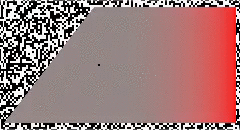
\includegraphics[width=0.3\linewidth]{movies/binding/colorgrdnt2_2fpsStatic} \caption{Task: judge whether the red color is paired with leftward tilt or rightward title.}\label{fig:redRightGreenLeft}
\end{figure}

In the above display, one can easily perceive that the color is alternating between green and red, and that the contour on the left is alternating rapidly between leftward tilt and rightward tilt. This means that the alternation rate does not exceed the temporal resolution of the early visual system - if it did, you would perceive just one color (yellow or brown).

Nevertheless, it is very difficult or impossible to judge which color, red or green, is presented at the same time as the leftward tilt \citep{holcombeEarlyBindingFeature2001}. When the animation is slowed to a rate much slower than about 200 ms per stimulus presentation however, the task becomes quite easy, as you can see below.

\begin{figure}
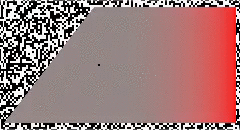
\includegraphics[width=0.3\linewidth]{movies/binding/colorgrdnt2_2fpsStatic} \caption{Task: judge whether the red color is paired with leftward tilt or rightward title.}\label{fig:unnamed-chunk-7}
\end{figure}

In the first movie, the temporal resolution of one's ability to pair the features was exceeded. The temporal dissociation here, and in other circumstances, between perceiving individual features and perceiving their pairing suggests that feature binding requires processes that take longer (have coarser temporal resolution) than those that provide perception of the individual features \citep{holcombeSeeingSlowSeeing2009, fujisakiCommonPerceptualTemporal2010b}.

In the above example, it is tempting to suggest that the dissociation results from a need to make a spatial shift of attention from one of the features' locations to the other in order to identify both before the other features are presented. However, the phenomenon can also occur with spatially superposed features, such as in the case of color and motion below:

While at the slow rate of the top row, it is easy to judge the pairing of motion direction and white/black color, it is very difficult in the middle row, where the speed is slightly faster.

The first to suggest this sort of thing reflected a general limit on temporal individuaation was Dutch guy

attend to the location of one feature first to identify it and
the colors and then of the

This phenomenon can also occur for features that are superposed.

not something specific to features

Thus, while early visual processing can deliver motion and color features even from stimuli that are temporally very close to each other, the processing required to judge which features are at the same time requires processing that fails when temporal proximity is very high

\hypertarget{loHighLevelLims}{%
\section{Low-level and high-level temporal limits}\label{loHighLevelLims}}

In the previous two sections I pointed out that while we can perceive the flicker in a rapidly changing light at rates as high as 60 Hz, some feature binding judgments begin to fail at 3 Hz. \citet{holcombeSeeingSlowSeeing2009} reviewed all the known temporal limits on human visual judgments, from flicker to binocular depth and motion as well as the binding of various features. These limits clustered into two groups, with one set of tasks limited to 8 Hz or below and another set with limits substantially greater than 8 Hz. The summary figure below, based on one in \citet{holcombeSeeingSlowSeeing2009} but with the addition of more recent evidence, highlights these two groups.

\begin{figure}
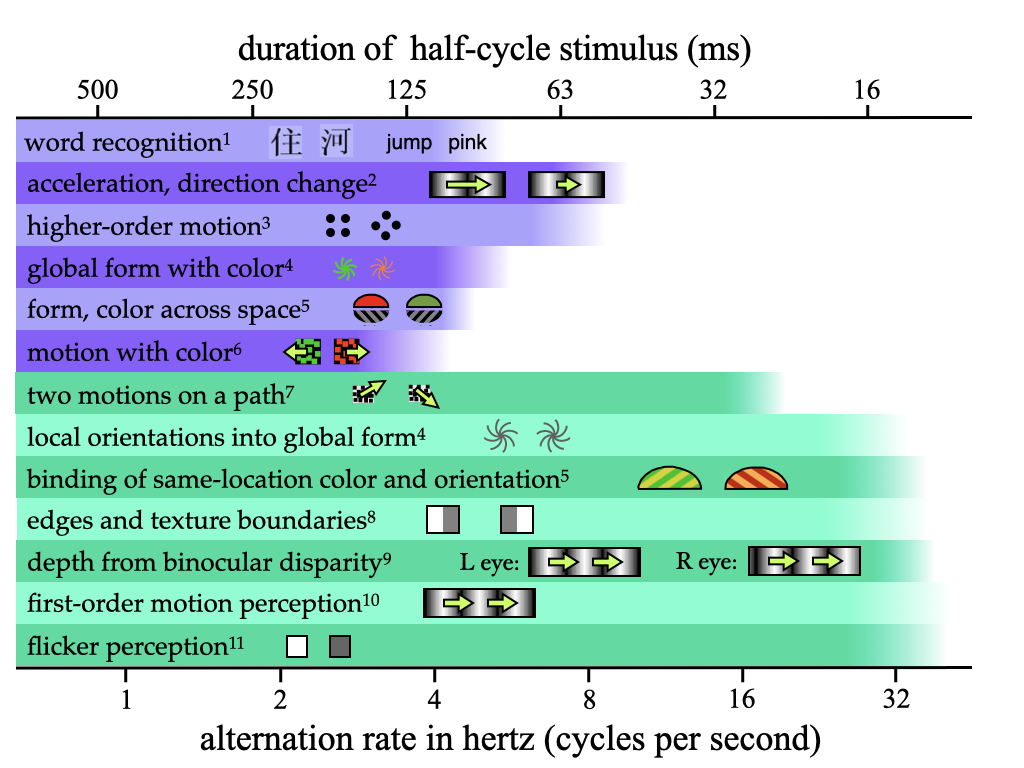
\includegraphics[width=1\linewidth]{imagesForRmd/temporalLimitsPerception/temporalLimits.001} \caption{Temporal limits on perception}\label{fig:temporalLims}
\end{figure}

1\citet{holcombeVisualBindingEnglish2007};
2\citet{werkhovenVisualProcessingOptic1992};
3\citet{verstratenLimitsAttentiveTracking2000};
4\citet{cliffordRapidGlobalForm2004};
5\citet{holcombeEarlyBindingFeature2001};
6\citet{arnoldPerceptualPairingColour2005};
7\citet{maruyaRapidEncodingRelationships2013};
8\citet{rogers-ramachandranPsychophysicalEvidenceBoundary1998};
9\citet{morganStereoscopicDepthPerception1995a};
10\citet{burrContrastSensitivityHigh1982};
11\citet{vonsegnerRaritaeLuminis1740}

The percepts limited to slow rates are likely to be computed by specialized perceptual mechanisms, whereas those limited to slow rates may require attentional selection and possibly parietal or temporal cortex to bind together two of the constituent features. This idea is schematized in Figure \ref{fig:slowFastBoxesArrows}.

\begin{figure}
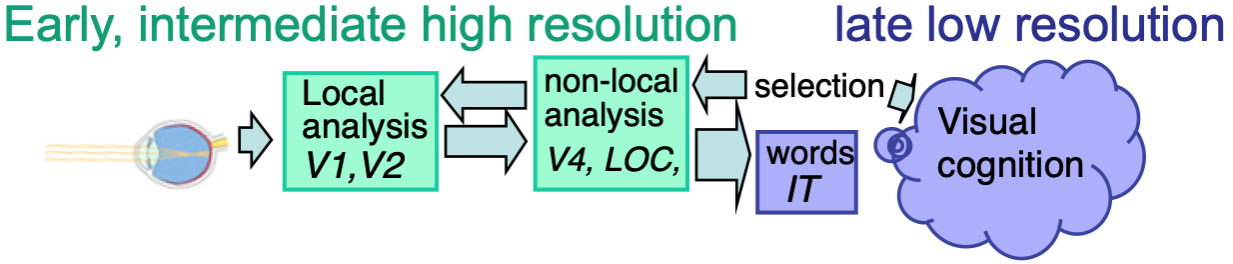
\includegraphics[width=1\linewidth]{imagesForRmd/temporalLimitsPerception/lowLevelFastHighLevelSlowBoxesArrows} \caption{Fast temporal limits on visual perception may reflect early and mid-level stages in the cortical processing hierarchy, while the slow limits seem to reflect later processing stages, often involving attentional selection.}\label{fig:slowFastBoxesArrows}
\end{figure}

\hypertarget{temporal-limits-on-tracking}{%
\section{Temporal limits on tracking}\label{temporal-limits-on-tracking}}

Where does object tracking fit into the above-reviewed temporal limits on visual judgments? A good starting point is the ambiguous apparent motion depicted in the ``higher-order motion'' part of Figure \ref{fig:slowFastBoxesArrows}. If those two frames are alternated, one can see apparent motion clockwise or counter-clockwise as both interpretations are equally viable. One can actually choose to see the figure to rotate clockwise or to rotate counter-clockwise, even while keeping the eyes fixed \citep{wertheimerExperimentelleStudienUber1912}. \citet{verstratenLimitsAttentiveTracking2000} found that the maximum alternation rate at which this could be done was between 4 and 8 Hz, depending on the participant. These alternation rates, 4 to 8 Hz, are also the rate at which a dot is presented at any given location. In a further experiment, \citet{verstratenLimitsAttentiveTracking2000} inserted frames between the two original frames to make the apparent motion unambiguously clockwise or counter-clockwise. They then used a tracking task, where participants had to follow with their attention one target disc as it stepped about the circular trajectory. None of their participants were able to do this when the flicker rate at an individual location exceeded 8 Hz. This truly seemed to be a temporal limit rather than a speed limit, because by varying the number of concurrently-presented discs and the number of intervening steps, the speed about the circle was varied, but what mattered most was the rate at which a disc appeared - the temporal frequency.

Importantly, these findings are not specific to jumpy apparent motion displays. \citet{verstratenLimitsAttentiveTracking2000} found a similar result with continuous motion of a grating, where temporal frequency is how often a bright (or dark) bar of the grating traverses any one location. Specifically, they used a circular sine-wave grating presented in an annulus. Participants fixated in the center, attempted to covertly track one light bar of the grating that was cued at the beginning of the trial, and performance fell to 75\% correct when the time between successive light bars of the grating was shorter than about 150 milliseconds (6.7 Hz) for the best of the three participants and about 238 ms (4 Hz) for the worst of the three.

\citet{holcombeSplittingAttentionReduces2013} found a similar result using discs rather than a grating - with 6 participants, once the discs were moving fast enough that two visited a location within 150 ms (6.6 Hz), tracking performance fell to a similar criterion (halfway to chance) as that used by \citet{verstratenLimitsAttentiveTracking2000}.

You can get a taste of this, first view the below movie, fixating on the dot in the center, and try to track the two targets that are initially white. If the movie isn't displayed properly, view it \href{movies/MOTmovies/temporalLimits/2targets3objectsPerArray.gif}{here}.
When the movie is at its beginning (when the speed readout at top right indicates 0.02 rps), one object in each of the two rings is drawn in white. These are the targets for you to track while you keep your gaze fixed on the dot in the center. As the speed gradually increases, try to keep tracking and see how fast it goes before you lose the targets.

\begin{figure}
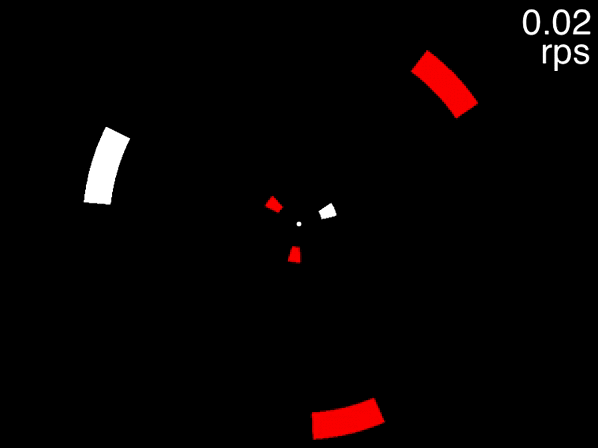
\includegraphics[width=1\linewidth]{movies/MOTmovies/temporalLimits/static_2targets3objectsPerArray} \caption{Task: fixate the white dot, track the initially-white targets, and note how fast you can track, using the speed in the upper right corner.}\label{fig:unnamed-chunk-9}
\end{figure}

Many people can track the targets even at the movie's fastest speed of approximately 0.6 rps (the exact speed it reached depends on your computer). This is to be expected, because at 0.6 rps, 3 objects corresponds to a an inter-object interval of 556 milliseconds, far higher than the temporal limit. The situation is quite different, however, for the below movie. If the movie isn't displayed properly, view it \href{movies/MOTmovies/temporalLimits/2targets9objectsPerArray.gif}{here}.

\begin{figure}
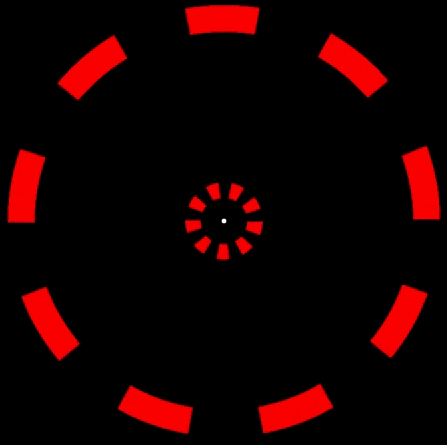
\includegraphics[width=1\linewidth]{movies/MOTmovies/temporalLimits/static_2targets9objectsPerArray} \caption{Fixate on the dot in the center, track the two targets that are initially white, and note the speed at which you are no longer able to track.}\label{fig:twoTargetsTemporalLimit}
\end{figure}

This movie uses the same speeds as the previous one. The only difference is that eight distractors are presented in each array instead of two. In this case people find that as the objects accelerate, very quickly they feel that they can no longer track the objects. Note that this is not due to spatial interference - only when the number of equidistant objects in an array exceeds 13 will spatial interference become significant \citetext{\citealp[p.11]{holcombeSplittingAttentionReduces2013}; \citealp{toetTwodimensionalShapeSpatial1992}; \citealp{pelliUncrowdedWindowObject2008}}.

Another way to think about temporal frequency limits such as this is that they reflect when temporal interference becomes strong due to close encounters in time. That is, just as increasing the spatial density of a display high enough will impair tracking due to spatial interference (crowding), a more dense display will also mean a higher temporal frequency, with an object and a distractor visiting the same spatial region in a short span of time.

This brings me to how \citet{verstratenLimitsAttentiveTracking2000} and \citet{holcombeSplittingAttentionReduces2013} established that the limit is a temporal one rather than a speed limit. They relied on the fact that a particular temporal frequency corresponds to different combinations of speed and spatial density, rather than a single speed as one would expect from a speed limit. The space-time diagrams in Figure \ref{fig:temporalResltnSushi} schematizes this, using the height of a pink rectangle to represent the temporal resolution of the tracking processes. At low stimulus speed and density the time between stimuli occupying any one spatial location is long, so tracking succeeds (top panel). When one increases either speed (middle panel) or density (lower panel), the interval between visits to each location decreases.

\begin{figure}
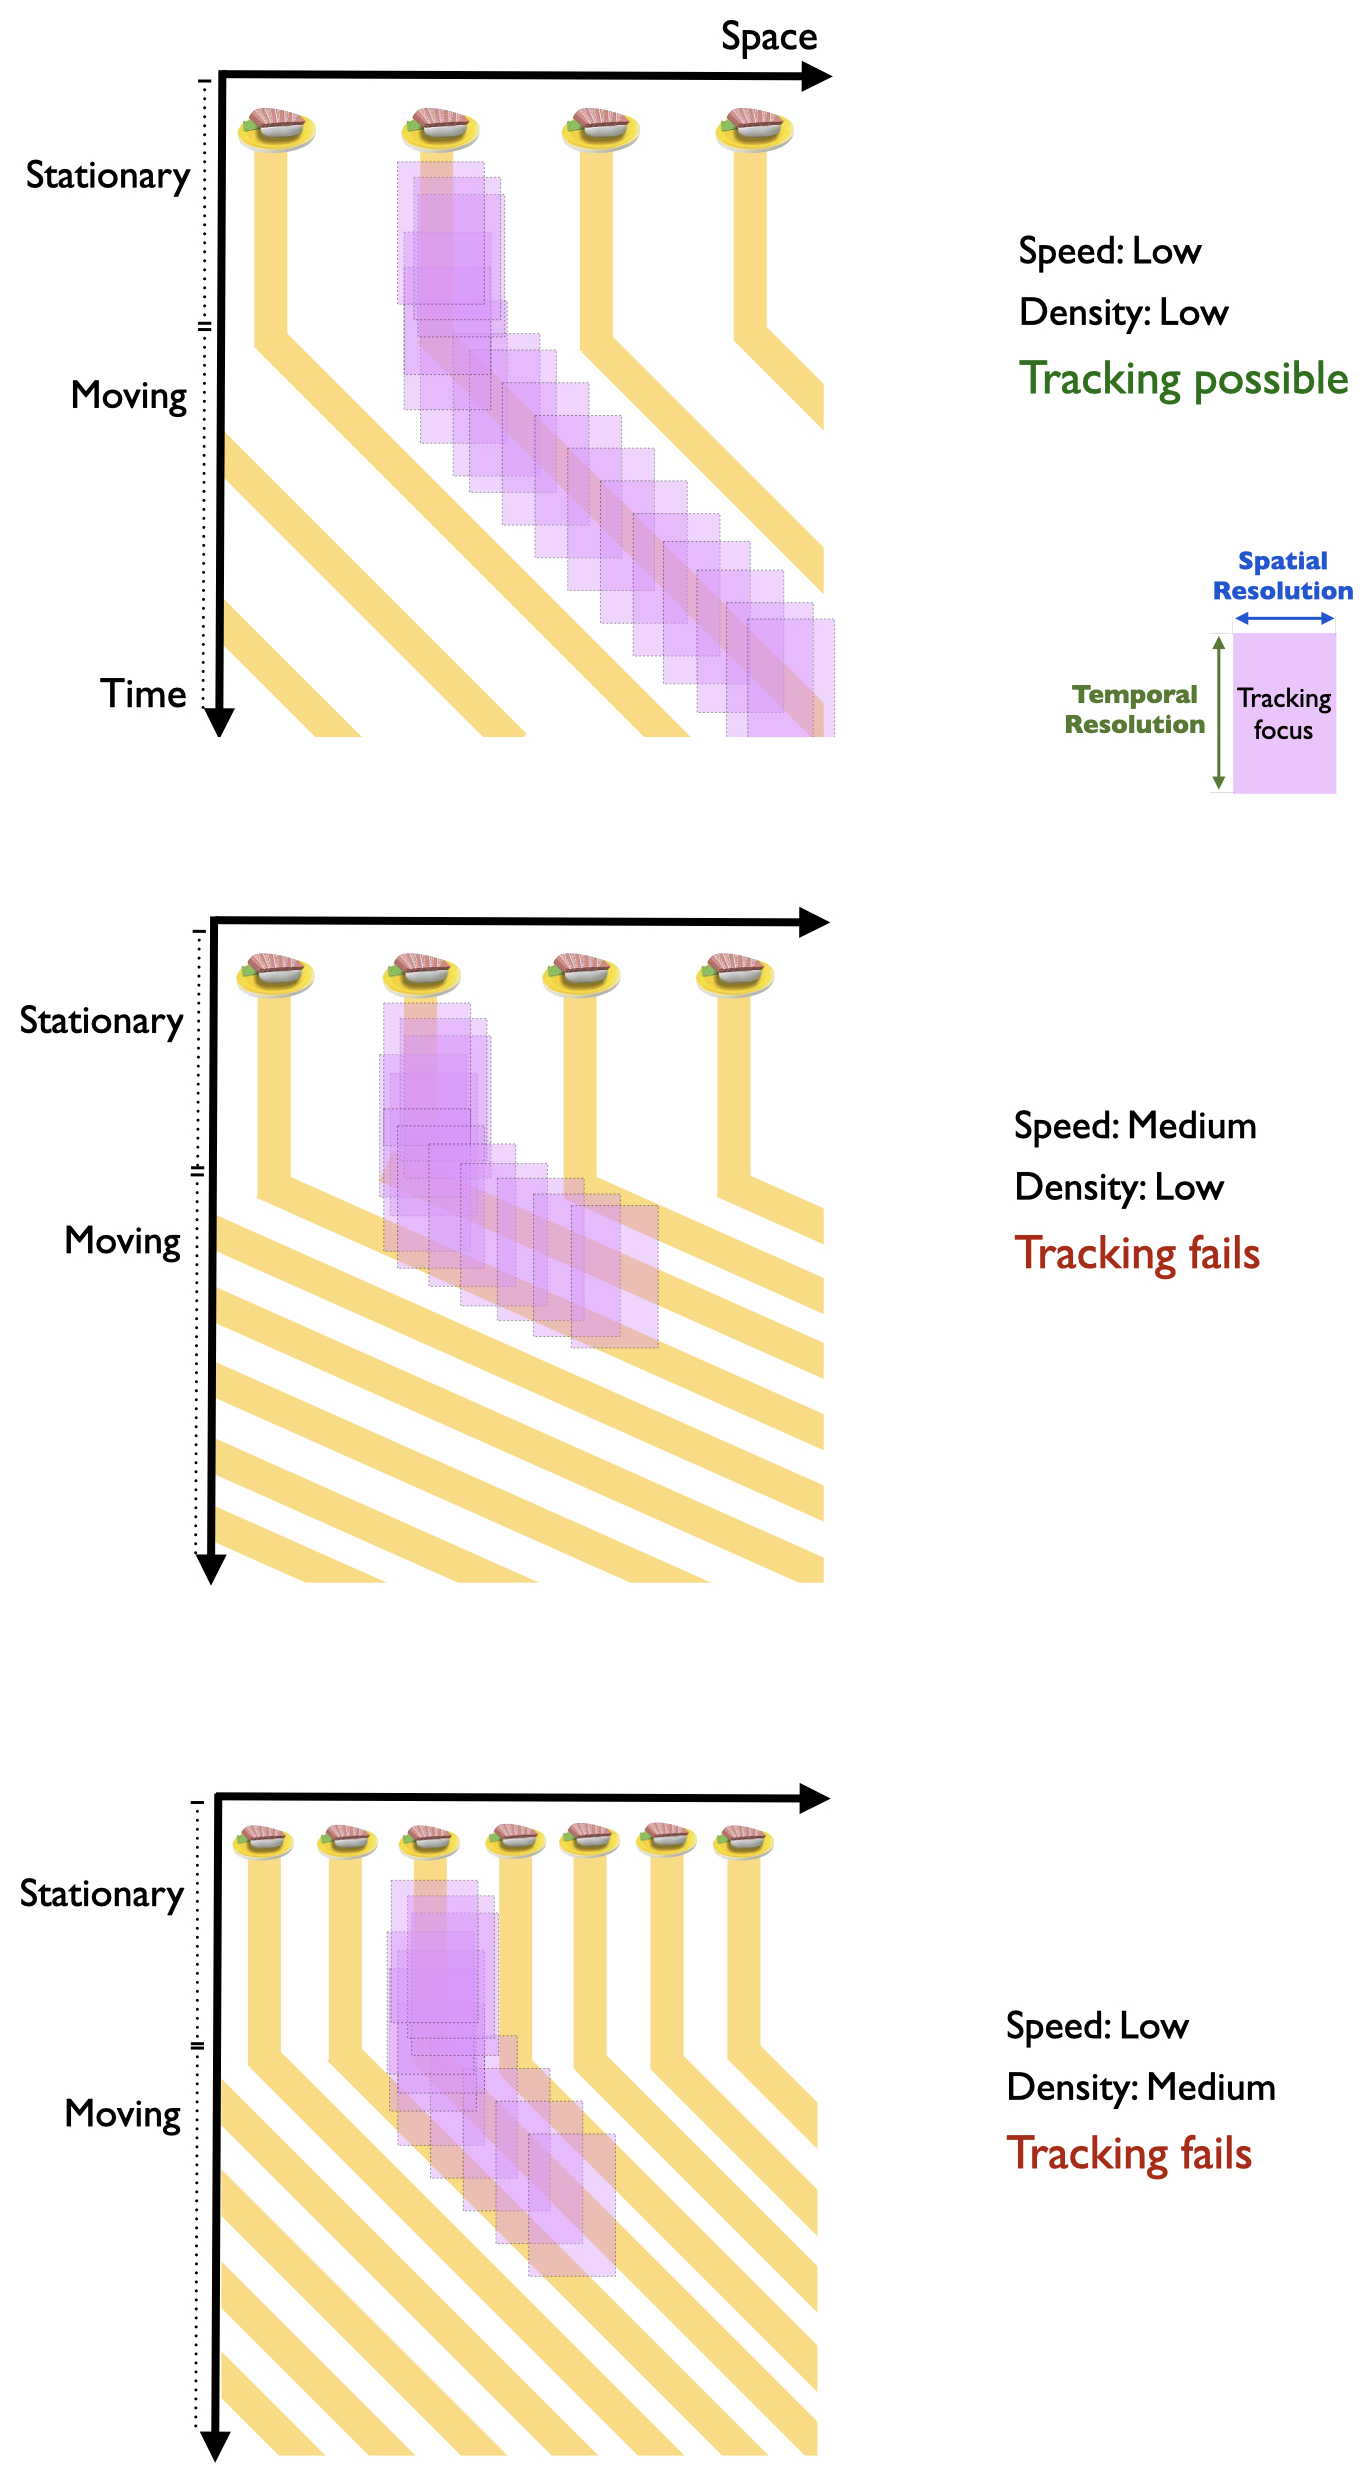
\includegraphics[width=0.8\linewidth]{imagesForRmd/spatialTempResltnSushi/temporalResltnSushi} \caption{The purple rectangle represents the spatial resolution (width) and temporal resolution (height) of tracking. Top panel: The space-time diagram schematizes a sushi train where one piece of sushi is designated as the target. Both density (number of sushi pieces) and speed is low. Tracking is possible because tracking is able to select a single piece of sushi. Middle panel: At medium speed, despite low density, tracking fails because temporal resolution is exceeded.  Bottom panel: At low speed but medium density, tracking fails because temporal resolution is exceeded.}\label{fig:temporalResltnSushi}
\end{figure}

Quantitatively, the rate of stimulation of each location is the product of speed and density. For a circular array, then, temporal frequency equals speed (in revolutions per second) times the number of discs in the circular array. This means that a temporal limit provides a quantitative prediction for the speed and density combinations that will correspond to participants' thresholds. This prediction was confirmed by the aforementioned studies. \citet{holcombeSplittingAttentionReduces2013}, for example, used four different inter-object spacings and many different speeds (speeds were adjusted by a staircase) to assess the speed threshold for each object spacing. The thresholds across the different spacings were close to that predicted by a 6.6 Hz limit. In a study discussed in more detail later, \citet{roudaiaDifferentEffectsAging2017} replicated this finding that thresholds were more consistent with a temporal frequency limit than with a speed limit - they tested two different spacings and found that the corresponding thresholds were more similar when expressed as temporal frequency than as speed.

The figure below summarises what we know about the limits on covertly tracking a single target.

\begin{figure}
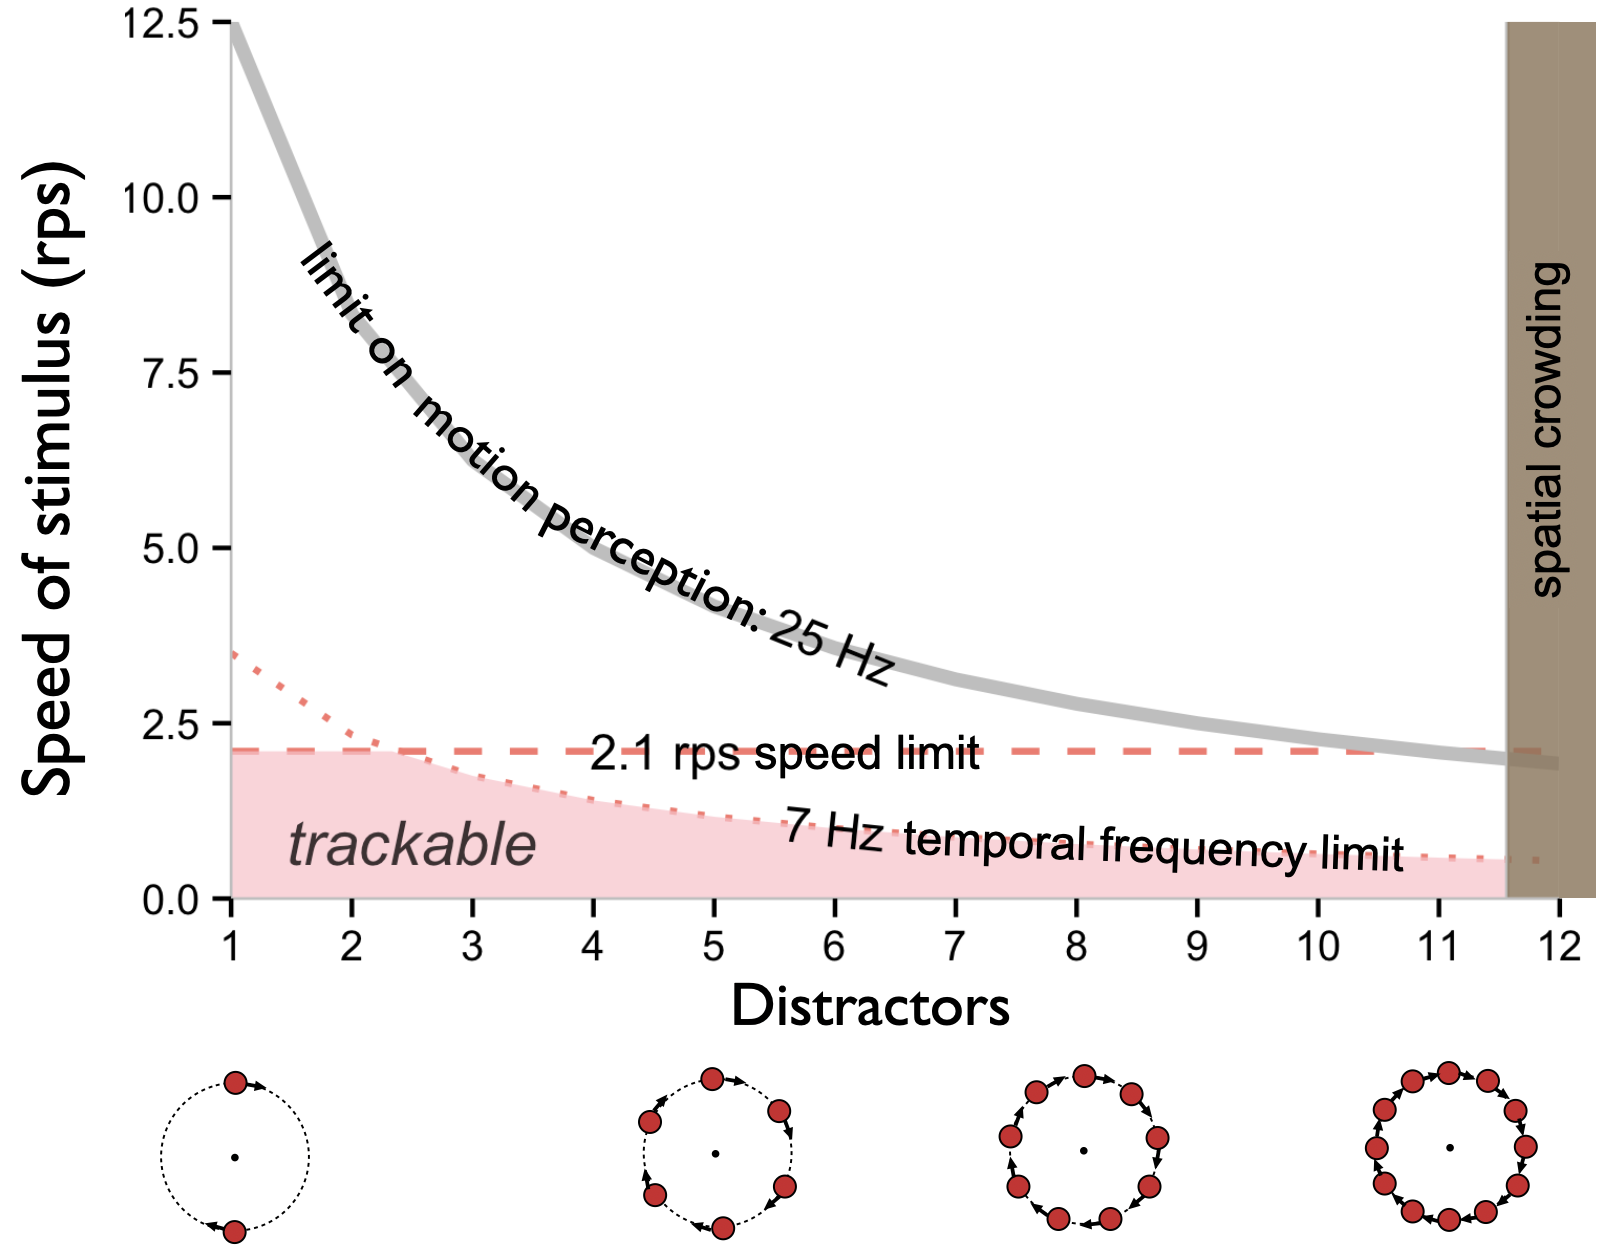
\includegraphics[width=1\linewidth]{imagesForRmd/trackingLimitsMotionLimitSchematic} \caption{Spatial and temporal limits on covertly tracking one object. UPDATE THIS IMAGE WITH BETTER NUMBERS IF REVIEWERS/EDITOR APPROVE OF THE FIGURE, including starting crowding at 13}\label{fig:singleTargetLimits}
\end{figure}

Based on the studies to date, the temporal frequency limit seems to vary substantially between different participants, but 7 Hz is near the top of the range and is used for Figure \ref{fig:singleTargetLimits}. For a circular array, 7 Hz corresponds to lower and lower speeds when more and more distractors are in the array. Note that these speeds are far, far below those that correspond to the limit on motion perception documented for drifting gratings - 25 Hz \citep{burrContrastSensitivityHigh1982}. Spatial crowding likely imposes another limit on tracking \citep{holcombeObjectTrackingAbsence2014, intriligatorSpatialResolutionVisual2001}, at a point far lower than the spatial acuity limit (not shown). Finally, as we will describe in the ``Speed limits'' section below, an actual speed limit (as opposed to a temporal limit) also seems to constrain tracking. The combination of these limits yields the combinations of speeds and number of distractors in a circular array indicated by the pink region.

These findings suggest an individuation limit wherein if a stimulus repeats at a particular location within a certain amount of time, about 120 ms if the limit is 8 Hz, the processes responsible for tracking fail. While they never studied tracking, \citet{vandegrindTemporalTransferProperties1973} anticipated this phenomenon to some extent. They coined the term ``Gestalt fusion'' to refer to how they saw the two phases of a flickering light as being perceived as a single thing when the flicker rate was above approximately 7 Hz. If this is an individuation limit, it might possibly have broader consequences than simply limiting tracking. It might be the reason for some or all of the other slow temporal limits reviewed in \ref{loHighLevelLims} above. Before considering that in detail, however, an important property that we have not discussed is how resource-intensive the temporal limit on tracking is.

\hypertarget{temporal-interference-is-highly-resource-intensive}{%
\section{Temporal interference is highly resource-intensive}\label{temporal-interference-is-highly-resource-intensive}}

In addition to replicating the finding of \citet{verstratenLimitsAttentiveTracking2000} of an approximately 7 Hz limit on attentional tracking, \citet{holcombeSplittingAttentionReduces2013} also investigated the limits on tracking with two targets and with three targets. They found that the temporal limit was markedly worse for higher target loads. Specifically, while when tracking one target, 143 ms had to elapse between when a target and a distractor visited a location (7 Hz), for two targets the threshold was about 238 ms, and for three targets it was about 385 ms. This dramatic effect of target load on temporal limit was replicated by \citet{roudaiaDifferentEffectsAging2017}, who also replicated the finding that these thresholds were more consistent with a temporal frequency limit than with a speed limit.

The effect of target load on temporal limit observed by \citet{roudaiaDifferentEffectsAging2017} was remarkably similar in size to the large effect found by \citet{holcombeSplittingAttentionReduces2013}. The eight participants tested by \citet{holcombeSplittingAttentionReduces2013} were all relatively young men, apart from two young women. \citet{roudaiaDifferentEffectsAging2017} tested both old and young participants, and reported a statistically significant difference. Among their young group, however, they tested only nine young men and nine young women, which for most known gender differences would be provide low statistical power, so the finding of a gender difference should be considered provisional.

\begin{verbatim}
## Warning in grid.Call.graphics(C_points, x$x, x$y, x$pch, x$size): conversion
## failure on '□' in 'mbcsToSbcs': dot substituted for <e2>
\end{verbatim}

\begin{verbatim}
## Warning in grid.Call.graphics(C_points, x$x, x$y, x$pch, x$size): conversion
## failure on '□' in 'mbcsToSbcs': dot substituted for <96>
\end{verbatim}

\begin{verbatim}
## Warning in grid.Call.graphics(C_points, x$x, x$y, x$pch, x$size): conversion
## failure on '□' in 'mbcsToSbcs': dot substituted for <a1>
\end{verbatim}

\begin{verbatim}
## Warning in grid.Call.graphics(C_points, x$x, x$y, x$pch, x$size): font metrics
## unknown for Unicode character U+25a1
\end{verbatim}

\begin{verbatim}
## Warning in grid.Call.graphics(C_points, x$x, x$y, x$pch, x$size): conversion
## failure on '□' in 'mbcsToSbcs': dot substituted for <e2>
\end{verbatim}

\begin{verbatim}
## Warning in grid.Call.graphics(C_points, x$x, x$y, x$pch, x$size): conversion
## failure on '□' in 'mbcsToSbcs': dot substituted for <96>
\end{verbatim}

\begin{verbatim}
## Warning in grid.Call.graphics(C_points, x$x, x$y, x$pch, x$size): conversion
## failure on '□' in 'mbcsToSbcs': dot substituted for <a1>
\end{verbatim}

\begin{verbatim}
## Warning in grid.Call.graphics(C_points, x$x, x$y, x$pch, x$size): font metrics
## unknown for Unicode character U+25a1
\end{verbatim}

\begin{verbatim}
## Warning in grid.Call.graphics(C_points, x$x, x$y, x$pch, x$size): conversion
## failure on '○' in 'mbcsToSbcs': dot substituted for <e2>
\end{verbatim}

\begin{verbatim}
## Warning in grid.Call.graphics(C_points, x$x, x$y, x$pch, x$size): conversion
## failure on '○' in 'mbcsToSbcs': dot substituted for <97>
\end{verbatim}

\begin{verbatim}
## Warning in grid.Call.graphics(C_points, x$x, x$y, x$pch, x$size): conversion
## failure on '○' in 'mbcsToSbcs': dot substituted for <8b>
\end{verbatim}

\begin{verbatim}
## Warning in grid.Call.graphics(C_points, x$x, x$y, x$pch, x$size): font metrics
## unknown for Unicode character U+25cb
\end{verbatim}

\begin{verbatim}
## Warning in grid.Call.graphics(C_points, x$x, x$y, x$pch, x$size): conversion
## failure on '○' in 'mbcsToSbcs': dot substituted for <e2>
\end{verbatim}

\begin{verbatim}
## Warning in grid.Call.graphics(C_points, x$x, x$y, x$pch, x$size): conversion
## failure on '○' in 'mbcsToSbcs': dot substituted for <97>
\end{verbatim}

\begin{verbatim}
## Warning in grid.Call.graphics(C_points, x$x, x$y, x$pch, x$size): conversion
## failure on '○' in 'mbcsToSbcs': dot substituted for <8b>
\end{verbatim}

\begin{verbatim}
## Warning in grid.Call.graphics(C_points, x$x, x$y, x$pch, x$size): font metrics
## unknown for Unicode character U+25cb
\end{verbatim}

\begin{verbatim}
## Warning in grid.Call.graphics(C_points, x$x, x$y, x$pch, x$size): conversion
## failure on '♂' in 'mbcsToSbcs': dot substituted for <e2>
\end{verbatim}

\begin{verbatim}
## Warning in grid.Call.graphics(C_points, x$x, x$y, x$pch, x$size): conversion
## failure on '♂' in 'mbcsToSbcs': dot substituted for <99>
\end{verbatim}

\begin{verbatim}
## Warning in grid.Call.graphics(C_points, x$x, x$y, x$pch, x$size): conversion
## failure on '♂' in 'mbcsToSbcs': dot substituted for <82>
\end{verbatim}

\begin{verbatim}
## Warning in grid.Call.graphics(C_points, x$x, x$y, x$pch, x$size): font metrics
## unknown for Unicode character U+2642
\end{verbatim}

\begin{verbatim}
## Warning in grid.Call.graphics(C_points, x$x, x$y, x$pch, x$size): conversion
## failure on '♂' in 'mbcsToSbcs': dot substituted for <e2>
\end{verbatim}

\begin{verbatim}
## Warning in grid.Call.graphics(C_points, x$x, x$y, x$pch, x$size): conversion
## failure on '♂' in 'mbcsToSbcs': dot substituted for <99>
\end{verbatim}

\begin{verbatim}
## Warning in grid.Call.graphics(C_points, x$x, x$y, x$pch, x$size): conversion
## failure on '♂' in 'mbcsToSbcs': dot substituted for <82>
\end{verbatim}

\begin{verbatim}
## Warning in grid.Call.graphics(C_points, x$x, x$y, x$pch, x$size): font metrics
## unknown for Unicode character U+2642
\end{verbatim}

\begin{verbatim}
## Warning in grid.Call.graphics(C_points, x$x, x$y, x$pch, x$size): conversion
## failure on '♂' in 'mbcsToSbcs': dot substituted for <e2>
\end{verbatim}

\begin{verbatim}
## Warning in grid.Call.graphics(C_points, x$x, x$y, x$pch, x$size): conversion
## failure on '♂' in 'mbcsToSbcs': dot substituted for <99>
\end{verbatim}

\begin{verbatim}
## Warning in grid.Call.graphics(C_points, x$x, x$y, x$pch, x$size): conversion
## failure on '♂' in 'mbcsToSbcs': dot substituted for <82>
\end{verbatim}

\begin{verbatim}
## Warning in grid.Call.graphics(C_points, x$x, x$y, x$pch, x$size): font metrics
## unknown for Unicode character U+2642
\end{verbatim}

\begin{verbatim}
## Warning in grid.Call.graphics(C_points, x$x, x$y, x$pch, x$size): conversion
## failure on '♀' in 'mbcsToSbcs': dot substituted for <e2>
\end{verbatim}

\begin{verbatim}
## Warning in grid.Call.graphics(C_points, x$x, x$y, x$pch, x$size): conversion
## failure on '♀' in 'mbcsToSbcs': dot substituted for <99>
\end{verbatim}

\begin{verbatim}
## Warning in grid.Call.graphics(C_points, x$x, x$y, x$pch, x$size): conversion
## failure on '♀' in 'mbcsToSbcs': dot substituted for <80>
\end{verbatim}

\begin{verbatim}
## Warning in grid.Call.graphics(C_points, x$x, x$y, x$pch, x$size): font metrics
## unknown for Unicode character U+2640
\end{verbatim}

\begin{verbatim}
## Warning in grid.Call.graphics(C_points, x$x, x$y, x$pch, x$size): conversion
## failure on '♀' in 'mbcsToSbcs': dot substituted for <e2>
\end{verbatim}

\begin{verbatim}
## Warning in grid.Call.graphics(C_points, x$x, x$y, x$pch, x$size): conversion
## failure on '♀' in 'mbcsToSbcs': dot substituted for <99>
\end{verbatim}

\begin{verbatim}
## Warning in grid.Call.graphics(C_points, x$x, x$y, x$pch, x$size): conversion
## failure on '♀' in 'mbcsToSbcs': dot substituted for <80>
\end{verbatim}

\begin{verbatim}
## Warning in grid.Call.graphics(C_points, x$x, x$y, x$pch, x$size): font metrics
## unknown for Unicode character U+2640
\end{verbatim}

\begin{verbatim}
## Warning in grid.Call.graphics(C_points, x$x, x$y, x$pch, x$size): conversion
## failure on '♀' in 'mbcsToSbcs': dot substituted for <e2>
\end{verbatim}

\begin{verbatim}
## Warning in grid.Call.graphics(C_points, x$x, x$y, x$pch, x$size): conversion
## failure on '♀' in 'mbcsToSbcs': dot substituted for <99>
\end{verbatim}

\begin{verbatim}
## Warning in grid.Call.graphics(C_points, x$x, x$y, x$pch, x$size): conversion
## failure on '♀' in 'mbcsToSbcs': dot substituted for <80>
\end{verbatim}

\begin{verbatim}
## Warning in grid.Call.graphics(C_points, x$x, x$y, x$pch, x$size): font metrics
## unknown for Unicode character U+2640
\end{verbatim}

\begin{verbatim}
## Warning in grid.Call.graphics(C_points, x$x, x$y, x$pch, x$size): conversion
## failure on '□' in 'mbcsToSbcs': dot substituted for <e2>
\end{verbatim}

\begin{verbatim}
## Warning in grid.Call.graphics(C_points, x$x, x$y, x$pch, x$size): conversion
## failure on '□' in 'mbcsToSbcs': dot substituted for <96>
\end{verbatim}

\begin{verbatim}
## Warning in grid.Call.graphics(C_points, x$x, x$y, x$pch, x$size): conversion
## failure on '□' in 'mbcsToSbcs': dot substituted for <a1>
\end{verbatim}

\begin{verbatim}
## Warning in grid.Call.graphics(C_points, x$x, x$y, x$pch, x$size): font metrics
## unknown for Unicode character U+25a1
\end{verbatim}

\begin{verbatim}
## Warning in grid.Call.graphics(C_points, x$x, x$y, x$pch, x$size): conversion
## failure on '○' in 'mbcsToSbcs': dot substituted for <e2>
\end{verbatim}

\begin{verbatim}
## Warning in grid.Call.graphics(C_points, x$x, x$y, x$pch, x$size): conversion
## failure on '○' in 'mbcsToSbcs': dot substituted for <97>
\end{verbatim}

\begin{verbatim}
## Warning in grid.Call.graphics(C_points, x$x, x$y, x$pch, x$size): conversion
## failure on '○' in 'mbcsToSbcs': dot substituted for <8b>
\end{verbatim}

\begin{verbatim}
## Warning in grid.Call.graphics(C_points, x$x, x$y, x$pch, x$size): font metrics
## unknown for Unicode character U+25cb
\end{verbatim}

\begin{verbatim}
## Warning in grid.Call.graphics(C_points, x$x, x$y, x$pch, x$size): conversion
## failure on '♂' in 'mbcsToSbcs': dot substituted for <e2>
\end{verbatim}

\begin{verbatim}
## Warning in grid.Call.graphics(C_points, x$x, x$y, x$pch, x$size): conversion
## failure on '♂' in 'mbcsToSbcs': dot substituted for <99>
\end{verbatim}

\begin{verbatim}
## Warning in grid.Call.graphics(C_points, x$x, x$y, x$pch, x$size): conversion
## failure on '♂' in 'mbcsToSbcs': dot substituted for <82>
\end{verbatim}

\begin{verbatim}
## Warning in grid.Call.graphics(C_points, x$x, x$y, x$pch, x$size): font metrics
## unknown for Unicode character U+2642
\end{verbatim}

\begin{verbatim}
## Warning in grid.Call.graphics(C_points, x$x, x$y, x$pch, x$size): conversion
## failure on '♀' in 'mbcsToSbcs': dot substituted for <e2>
\end{verbatim}

\begin{verbatim}
## Warning in grid.Call.graphics(C_points, x$x, x$y, x$pch, x$size): conversion
## failure on '♀' in 'mbcsToSbcs': dot substituted for <99>
\end{verbatim}

\begin{verbatim}
## Warning in grid.Call.graphics(C_points, x$x, x$y, x$pch, x$size): conversion
## failure on '♀' in 'mbcsToSbcs': dot substituted for <80>
\end{verbatim}

\begin{verbatim}
## Warning in grid.Call.graphics(C_points, x$x, x$y, x$pch, x$size): font metrics
## unknown for Unicode character U+2640
\end{verbatim}

\begin{figure}
\centering
\includegraphics{tracking-review_files/figure-latex/trackingLimitsReview-1.pdf}
\caption{\label{fig:trackingLimitsReview}The results of the two experiments of Holcombe \& Chen (2013) plotted with the comparable sample (young people) of Roudaia \& Faubert (2017). The data symbols are horizontally offset to avoid overlap.}
\end{figure}

In each of the four datasets plotted (and also in the data from the old participants excluded because of outliers), the temporal limit decreases dramatically with increasing target load. Of all the effects of increasing target load that we have discussed, this one may be the largest.

Attentional tracking is a complex task - in section \ref{whichAspects}, six factors likely to affect tracking performance were listed. However, some of these factors might affect practically any task; it is those that are most resource-intensive, and thus most limit our capacity, that should be most illuminating for understanding tracking processes.

From the rather unconstrained trajectories used in most MOT studies, researchers were unable to make strong inferences about how target load was adversely affecting performance. For example, it was necessary to carefully control the distances between objects to disconfirm the suggestion that spatial interference even beyond the crowding range was the primary determinant of the effect of tracking load \citep{holcombeObjectTrackingAbsence2014, holcombeCommentCapacityLimits2019}.

For temporal interference, the evidence is strong that it is dramatically increased by target load. This leads to two important questions. The first is: what does this effect tell us about how tracking works? Discussion of this is deferred to the \ref{serialOrParallel} section, but in short, it supports serial switching theories of tracking.

The second question is: what role does temporal interference play in typical MOT displays that use more linear trajectories? Unfortunately, none appear to have done so for temporal interference. And some of the evidence from studies that set out to investigate the role of spatial proximity might alternatively be explained by temporal proximity \citep[e.g.,][]{baeCloseEncountersDistracting2012}- in typical MOT displays, spatial proximity is likely to be highly correlated with temporal proximity.

\hypertarget{relation-to-other-temporal-limits}{%
\section{Relation to other temporal limits}\label{relation-to-other-temporal-limits}}

A plausible interpretation of the temporal limit on tracking is that it is an attentional selection individuation limit. Above the limit, stimuli cannot be individually selected by attention for processing by higher-level, limited-capacity processes such as cognition. This could prevent successful performance of many, or all, of the tasks in the slow group of Figure \ref{fig:temporalLims}. For example, to correctly identify that red is paired with leftward-tilted in \ref{fig:redRightGreenLeft}, both the color and the orientation have to be identified. If attention is unable to select an individual color and orientation and instead has access only to two or more successive frames, then from the perspective of higher-level processes, both colors and both shapes were essentially presented simultaneously. This is illustrated in Figure \ref{fig:temporalresolutionwaterworks}.

\begin{figure}
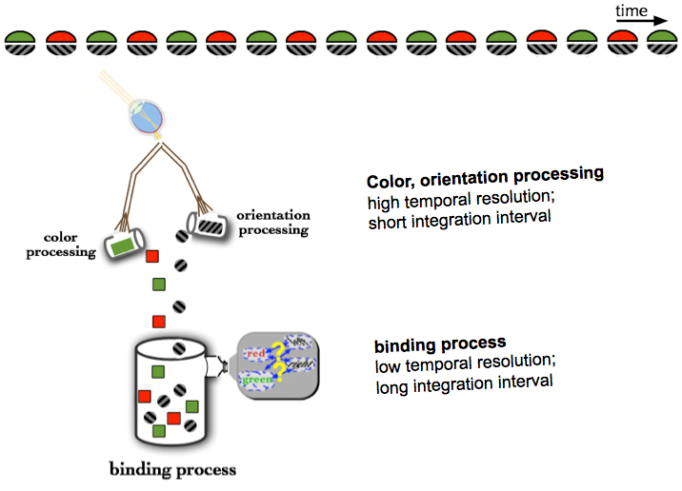
\includegraphics[width=0.8\linewidth]{imagesForRmd/temporalLimitsPerception/temporalresolutionwaterworks} \caption{A rapidly alternating color-orientation pairing stimulus (top) is processed first by high temporal resolution feature processors, which independently determine the color and orientation. Subsequently the pairing of the two features is determined by a process that, because it is low temporal resolution, unfortunately 'sees' multiple colors and orientations simultaneously.}\label{fig:temporalresolutionwaterworks}
\end{figure}

While the temporal limit on binding for this and related tasks is less than 3 Hz \citep{holcombeEarlyBindingFeature2001, arnoldPerceptualPairingColour2005}, the tracking limit for one target is significantly higher, close to 7 Hz \ref{fig:trackingLimitsReview}. The reason for this may be that while both tasks require individuation, the binding tasks require additional processing such as labeling of the features \citep{holcombeEarlyBindingFeature2001, fujisakiCommonPerceptualTemporal2010}. This theory is consistent with the evidence reviewed in \ref{identity} that encoding of features (such as color or orientation) does not occur in basic tracking. The successive locations of a tracked object must be paired, but this may be faster than other forms of binding, both because feature encoding is not required and possibly because it may piggy-back on motion perception.

\citet{marinovicAttentionaltrackingAcuityModulated2013} investigated the role of motion mechanisms with an adaptation experiment in which participants were exposed to a prolonged period of either slow or fast motion. Exposure to slow motion decreased the participants' maximum tracking speed, while exposure to fast motion actually increased it. Note that this is opposite in direction to what one might expect from other instances of sensory adaptation, wherein adaptation to high spatial frequency, for example, \emph{reduces} the maximum spatial frequency one can perceive, which is thought to be because the underlying mechanism becomes less responsive.

\citet{marinovicAttentionaltrackingAcuityModulated2013} theorized that this surprising effect reflected changes in the relative contribution of the two types of spatiotemporal filters thought to mediate speed perception. Specifically, \citet{marinovicAttentionaltrackingAcuityModulated2013} suggested that the low-pass filters are needed to individuate a target from the distractors, because, they said, only the low-pass filters have small enough receptive fields. On that basis, adaptation to slow motion reduces the temporal limit on tracking. They further proposed that adapting to fast motion adapts the band-pass temporal frequency filters that, being large, tend to group the target with the distractors, and thus reducing their responsiveness is a good thing. This account seems plausible for the stimulus they used, as the moving discs were quite close to each other, as there were twelve of them sharing the circular trajectory. I am not sure whether the same can be said if there were only six discs in the trajectory. Unfortunately \citet{marinovicAttentionaltrackingAcuityModulated2013} did not test this. They also did not test whether the speed limit, as opposed to the temporal limit, was changed by adaptation; this could be investigated by using two or three discs in the circular trajectory. The finding of \citet{marinovicAttentionaltrackingAcuityModulated2013} is an important one as further investigation seems likely to provide additional insights.

\hypertarget{speed-limits}{%
\section{Speed limits}\label{speed-limits}}

We have seen that the apparent speed limits on tracking in dense displays may actually be caused by temporal limits. This is because when there are a lot of objects in a display, at high object speeds both targets and distractors may occupy a particular location within three or four hundred milliseconds, which can impair or prevent tracking. Temporal interference is less of an issue when the targets and distractors are kept very far apart from each other.

When using a circular trajectory with just one target and one distractor on opposite sides, such that the distractor did not replace the target very quickly, \citet{verstratenLimitsAttentiveTracking2000} found evidence that tracking was truly limited by speed rather than by temporal interference. What this was that the maximum speed at which participants could track was much lower than what was predicted by the 7 Hz limit found when several distractors shared the circular trajectory with the target. With one target and one distractor, the 7 Hz limit should result in a speed threshold of 3.5 revolutions per second. Instead, participants' thresholds were on average less than 2 revolutions per second. My lab found a very similar result \citep{holcombeSplittingAttentionReduces2013}. When we tested with 5, 8, or 12 distractors, the speed limit was close to that predicted by a 7 Hz temporal limit. But when there were only 2 distractors in the array, the average speed limit was only 1.7 rps, rather than 3.5 rps predicted by a 7 Hz limit.

It seems, then that tracking of a single object is limited both by a speed limit of about 2 revolutions per second and by a temporal limit of about 7 Hz. The computer screens that were used for testing had refresh rates of 160 Hz, and when the speed of an object is very fast, one can see gaps between the successive frames, which conceivably could be contributing to the speed limit. However, when Wei-Ying Chen and I used a mechanical device rather than an intermittent computer display, we found a speed limit that was only slightly faster, about 2.3 rps \citep{holcombeSpeedLimitAttentional}.

Changing the radius of the circular trajectory in experiments like these yielded a truly remarkable finding. Well, \citet{verstratenLimitsAttentiveTracking2000} mentioned that for their experiments where participants had to track one bar of a circular 2-cycle grating, they also informally tested annular gratings of different sizes. When the grating was larger, the length of the path traveled by the bar when making one revolution was, of course, longer. One would therefore expect that the speed threshold, when expressed in revolutions per second, should decrease in proportion to the radius of the grating. Consider that a grating of radius 2 deg has twice the circumference as that of a 1 deg radius grating, so the revolutions per second should be halved in order for a bar to travel the same distance in the same amount of time. However, \citet{verstratenLimitsAttentiveTracking2000} said that they saw no change in the speed limit in terms of rps. That is, participants could track an object moving twice as fast when the trajectory had a larger radius.

Wei-Ying Chen and I also found that the speed threshold, when expressed in revolutions per second, was robust to the increases in length of the trajectory associated with larger radii \citep{holcombeSplittingAttentionReduces2013, holcombeExhaustingAttentionalTracking2012}, despite the substantial increase in speed in terms of linear distance traveled. We will therefore refer to the speed limit as an angular speed limit.

What does this mean for the processes that underlie tracking? Conceivably, the limit could be imposed by the \emph{cortical} distance traveled, as the amount of retinotopic cortex per deg of visual angle may diminish linearly with eccentricity. However, for the limit to stay close to constant would require that the scaling constant be equal to one, but empirically this does not seem to be the case, based both on psychophysical and physiological measures \citep{strasburgerPeripheralVisionPattern2011}. Another possibility is we might call the costly hemifield-crossing theory. Doubling the revolutions per second doubles the rate of crossing the vertical meridian, and crossing that meridian is known to impair tracking \citep{strongHemifieldspecificControlSpatial2020}. If so, a faster limit should be found for trajectories that do not cross the vertical meridian, but in an unpublished experiment \citep{holcombeSpeedLimitAttentional}, this was not found. Finally, \citet{verstratenLimitsAttentiveTracking2000} suggested that the limit may coincide with that found for mental rotation of objects \citep{cooperMentalTransformationsVisual1976}, so possibly the same processes limit both.

Other than \citet{verstratenLimitsAttentiveTracking2000} and myself and Chen, no tracking researchers appear to have grappled with the angular speed limit, or mentioned it in any published papers. Instead, MOT researchers continue to write as if tracking is limited by linear distance traveled per unit time, not by revolutions per second or by temporal interference. Admittedly, the speed limit may have little effect in conventional MOT displays with linear trajectories, because for the speeds tested in all or practically all such experiments, objects probably take longer than a second to ever move a full revolution around a point in the display. However, many recent papers use circular trajectories, where the angular speed limit may come into play, although again they tend to use speeds slower than 1 rps \citep[e.g.][\citet{carlsonQuadranticDeficitReveals2007}]{maechlerAttentionalTrackingTakes2021}.

Is the angular speed limit caused by a more structural limitation, what \citet{normanDatalimitedResourcelimitedProcesses1975} called data-limited, or is it resource intensive like the temporal frequency limit? If it is resource intensive, the speed limit should be lower when more targets are tracked, as that would result in less resource available per target. \citet{holcombeSplittingAttentionReduces2013} did document an associated decline in speed thresholds, from 1.7 rps with one target to 1.2 rps with two targets and 0.8 rps with three targets. Unfortunately, however, it is difficult to discern whether this reduction is due to a reduction in the actual speed limit, or instead was caused by the previously-documented decline in temporal frequency limit. The problem is that the temporal frequency limit with two targets (approximately 4 Hz) corresponds to a speed, with three objects in a trajectory, below that of the one-target speed limit, so it is difficult to know whether the speed threshold reflects a decline in both the temporal limit and the speed limit or just the temporal limit.

Using fMRI, \citet{shimNumberAttentionalFoci2010} investigated the brain areas associated with multiple object tracking, and varied objects' speeds. If higher speeds consumed more of the tracking resource, one might expect that higher speeds would increase the activation in the same areas that increase in activation with more targets. \citet{shimNumberAttentionalFoci2010} identified a parietal region that increased in activation with the number of targets. However, there was no increase in activation of any parietal area with target speed. In a whole-brain analysis, however, \citet{shimNumberAttentionalFoci2010} did find some scattered voxels whose activity increased with speed, including the frontal eye field, which is often associated with attentional tasks. \citet{howeUsingFMRIDistinguish2009} also found strong FEF activation in MOT. They did not vary speed, but did compare tracking moving targets to monitoring targets that were stationary, and found that that comparison also yielded strong FEF activation. They suggested that given the FEF's involvement in eye movements, the activation might reflect suppression of eye movements. Although they did not cite any evidence that suppression of eye movements is more demanding for tracked moving targets than for monitored stationary targets, that seems highly plausible.

\hypertarget{putting-it-all-together}{%
\section{Putting it all together}\label{putting-it-all-together}}

The temporal interference and associated temporal limits on tracking are clearly highly resource-intensive. Tracking three targets rather than one almost triples the severity of the temporal limit. We will discuss the theoretical implications in a subsequent section. Tracking is also constrained by a speed limit, but we do not yet know whether the speed limit decreases with more targets or is instead a fixed limit. We also do not understand the nature of the speed limit - whether it is truly a rotational limit and how it relates to other mental processes.

\begin{figure}
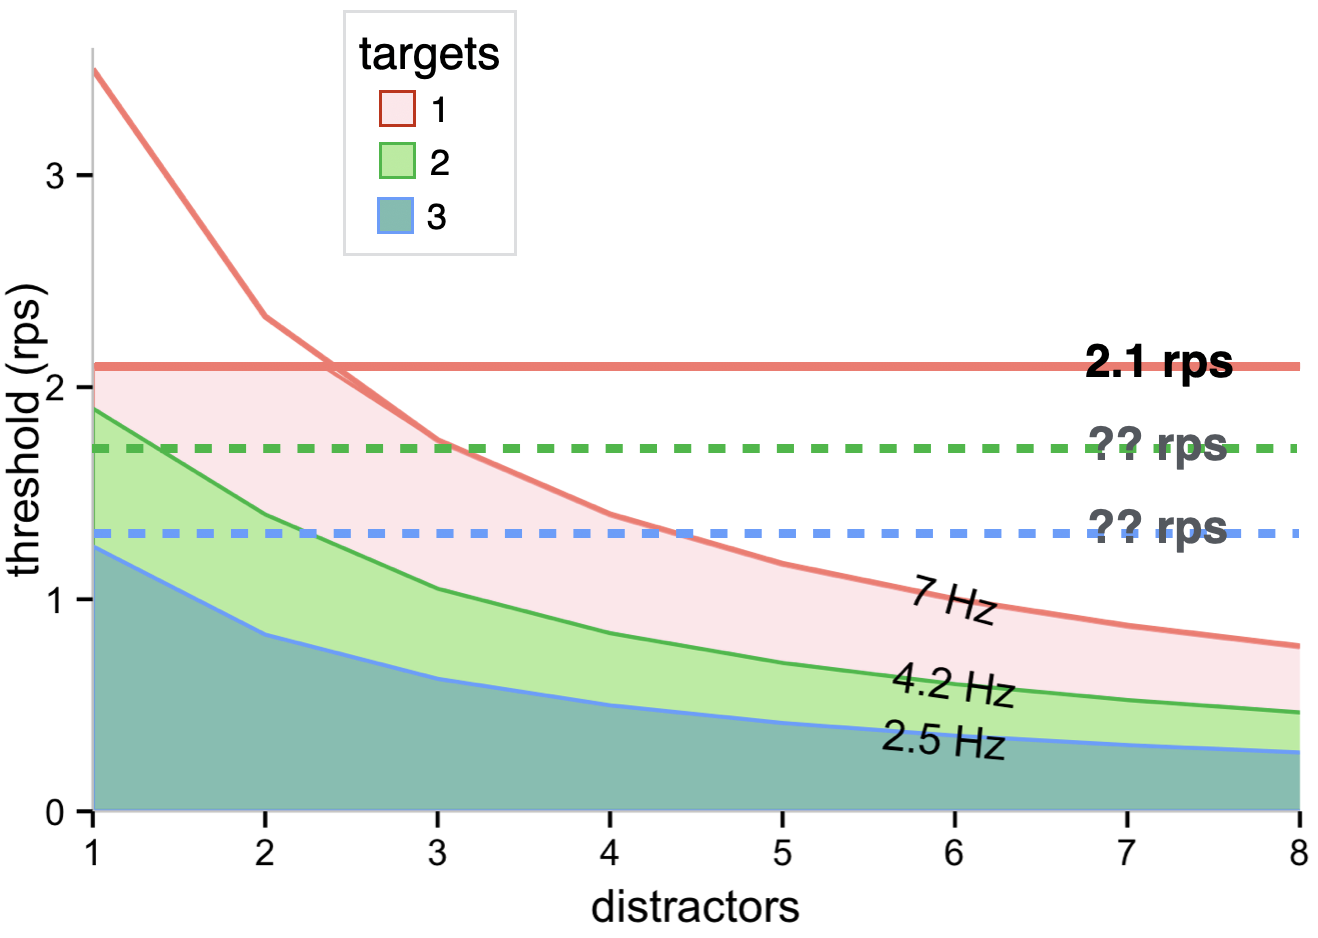
\includegraphics[width=1\linewidth]{imagesForRmd/temporalAndSpeedLimits} \caption{Spatial and temporal limits on covertly tracking one, two, and three targets. }\label{fig:unnamed-chunk-10}
\end{figure}

\hypertarget{twoBrains}{%
\chapter{Two brains or one?}\label{twoBrains}}

A human brain can be thought of as made up of two brains, a left and a right, just as we have two legs and two hands.
Much of sensory and perceptual processing is very specific to the two halves of the cortex, but more cognitive functions such as declarative memory benefit from a very tight integration. Indeed, this integration is extensive enough that the comparison of our two hemispheres to our two hands is misleading.

Our conscious experience, too, is highly unified. We experience no discontinuity when the movement of our eyes, or of an object, cause an object to shift from one hemifield, where it is processed predominantly by one hemisphere, to the other hemifield. Communication between the two hemispheres happens rapidly and continuously, and there is no good evidence that exercises designed to insure both hemispheres process stimuli have any benefit for learning.

In ``split-brain'' patients, many of the connections between the hemispheres have been lost. Despite the loss of these connections, such patients can still perform visual search in both hemifields, indicating that both hemispheres have the capacity to do that task. Indeed, when split-brain patients are asked to search for a target among many distractor objects, spreading the load by distributing the distractors across the two hemifields can yield a large benefit, suggesting that the two hemispheres in these patients carry out their searches independently \citep{luckIndependentAttentionalScanning1994a}. For intact individuals, no such advantage is seen, suggesting that the processes that evaluate each stimulus for whether it is the target are integrated across the hemispheres into a single attentional focus \citep{luckIndependentHemisphericAttentional1989}.

While performance in search and other behaviors typically shows a tight inter-hemispheric integration, the two hemispheres do specialize for certain functions. The left hemisphere specializes in language functions such as reading, while the right hemisphere is better at recognizing faces. A behavioral consequence of this is that response times for a face recognition task are slightly faster when the stimulus is presented wholly in the left hemifield (to the right hemisphere) than when it is presented wholly in the right hemifield, whereas the opposite is found for word reading \citep{rizzolattiOppositeSuperioritiesRight1971}. However, with extended time to process a stimulus, such behavioral asymmetries can disappear as the information from one hemisphere is communicated to the other.

In the performance of most perceptual and attentional tasks, then, in humans with an intact brain there is little sign that that brain is divided into two halves. Multiple object tracking, however, constitutes a major exception to this. This tells us that the limited resource that determines how many objects one can keep track of resides largely with a process that operates independently in the two hemispheres.

\hypertarget{the-extraordinary-hemifield-independence-of-object-tracking}{%
\section{The extraordinary hemifield independence of object tracking}\label{the-extraordinary-hemifield-independence-of-object-tracking}}

In 2005, George Alvarez \& Patrick Cavanagh reported a stunning finding. In an MOT task, they used objects that resembled spinning pinwheels. An individual bar of each object could be designated as a target. Performance in a two-target (one bar of each of two different pinwheels) condition was contrasted with that for a one-target condition \citep{alvarezIndependentResourcesAttentional2005}. When the second target was positioned in the same hemifield as the first target, accuracy in the two-target condition was much worse (89\% vs.~63\%). Remarkably, however, when the second target belonged to a pinwheel located in the opposite hemifield, there was very little performance decrement - accuracy was 93\% in the one-target condition, and 90\% correct in the two-target condition. This suggests that the processes that limit successful tracking in this task are largely specific to each hemifield.

It was already known that sensory processing and quite a lot of perceptual processing occurs independently in each hemisphere. What is surprising is that a highly limited-capacity processing ability would be hemisphere-independent. Such capacities were traditionally thought to be among the processes that are tightly integrated across the two hemispheres, forming a single resource ``pool'', not two independent limits. We will get back to this point, first we'll examine more extensively the evidence for hemispheric independence of object tracking.

\hypertarget{quantitative-estimates-of-independence}{%
\section{Quantitative estimates of independence}\label{quantitative-estimates-of-independence}}

The hemispheric independence of a task can be quantified. Imagine that adding a second stimulus to a hemifield reduces performance by 20 percentage points, but adding that stimulus to the other hemifield reduces performance by only 5 percentage points. One can quantify the hemispheric independence, then, as (20-5) / 20 = 75\% hemifield independence. Ideally, however, one would not use raw accuracy but instead would correct for the accuracy one can achieve by guessing. When \href{https://github.com/alexholcombe/tracking-review/blob/main/twoBrainsOrOne.Rmd}{applying such a calculation} to the \citet{alvarezIndependentResourcesAttentional2005} results, the estimated level of independence is very high: 88\% independence in one of their experiments, and 92\% in the other.

\citet{alvarezIndependentResourcesAttentional2005} themselves, like most others who have investigated this question, did not do these calculations. \citet{alvarezIndependentResourcesAttentional2005} calculated expected performance if the hemifields are in fact completely independent, and reported that performance was not statistically significantly worse than that figure. They then suggested that there was complete independence, but this is based on the common fallacy of concluding a null hypothesis is true when the evidence does not reject it at a p\textless.05 level \citep{aczelQuantifyingSupportNull2018}. That is, for the null hypothesis they started with their conclusion of complete independence, and then affirmed this conclusion on the basis of not finding much evidence against it. Nevertheless, their data do suggest hemispheric independence of approximately 90\%. In a study with similar methods, \citet{hudsonHemifieldEffectsMultiple2012} found 65\% independence (they did not calculate a number, so this is \href{https://github.com/alexholcombe/tracking-review/blob/main/twoBrainsOrOne.Rmd}{my calculation}).

Some of the follow-up studies in this area have not included enough conditions to quantify the degree of independence, or confounded distribution of the targets to two hemifields with greater distance among them, such that any benefit might have been due to less spatial crowding interference, a phenomenon discussed in section \ref{spatialInterference}.

\citet{holcombeExhaustingAttentionalTracking2012} and \citet{chenResourceDemandsObject2013} found similar results with a slightly different approach based on speed thresholds, which are discussed in section \ref{speedAndTime}. The findings were compatible with approximately 100\% hemifield independence or a bit less. \citet{shimNumberAttentionalFoci2010} and \citet{stormerWithinhemifieldCompetitionEarly2014} also found evidence for a substantial bilateral advantage compared to adding a target in the same hemifield.

These findings of hemispheric independence has not replicated in all circumstances \citep[e.g.,][]{shimSpatialSeparationTargets2008} , but the successful replications strongly suggest that at least in some circumstances, tracking does occur mostly independently in the two hemispheres. I say ``mostly independently'' rather than suggesting complete independence because each individual study has too much statistical uncertainty to rule out a figure such as 75\% independence, even when its mean suggests a higher degree of independence.

\citet{shimSpatialSeparationTargets2008} suggested that the reason they did not find evidence for hemifield independence is that they used only two targets, whereas according to them the original \citet{alvarezIndependentResourcesAttentional2005} report of hemifield independence used four targets. This is unlikely to be the reason for the discrepancy, however, because in their E1 and E2 \citet{alvarezIndependentResourcesAttentional2005} did find evidence for hemifield independence using just two targets, as did \citet{holcombeExhaustingAttentionalTracking2012} and \citet{stormerWithinhemifieldCompetitionEarly2014}. The \citet{shimSpatialSeparationTargets2008} data may have been afflicted by a ceiling effect, as accuracy was over 85\% correct in all conditions in their experiment.

A limitation of deriving hemispheric independence from accuracy is that they depend on the assumption that if a person can only track one target, if one then adds a second target, the person will succeed just as often in tracking one of them. But my introspective experience indicates that in some circumstances, if one tries to track both targets, one will fail at both, and thus one is better off only trying to track one. The reason for this may be that a certain amount of resource is needed to track a target, and so if neither target is allocated that much resource, tracking will fail for both. Evidence for this was provided by \citet{chenResourceDemandsObject2013}. In the terminology introduced by \citet{normanDatalimitedResourcelimitedProcesses1975}, the resource function that relates the proportion of attentional resource to accuracy falls below a straight line. This means that quantitative estimates of hemispheric independence will be overestimates, particularly in circumstances where the participants do not realize they may be better off focusing their efforts on tracking fewer targets than the number they have been told to track.

\citet{carlsonQuadranticDeficitReveals2007} found evidence not only for hemifield independence but also quadrant-level independence, which they attributed to the partial separation of the retinotopic quadrant representations in areas V2 and V3. Using different stimuli, \citet{shimSpatialSeparationTargets2008} and \citet{holcombeObjectTrackingAbsence2014} did not, however, find evidence for this: they did not find evidence for a deficit when two targets were positioned in the same quadrant compared to different quadrants but in the same hemifield. More work on this topic should be done.

\hypertarget{some-tracking-resources-are-not-hemifield-specific}{%
\section{Some tracking resources are NOT hemifield-specific}\label{some-tracking-resources-are-not-hemifield-specific}}

One attentional process that is not hemifield-specific is feature attention, for example attention to color. When a participant is told to look for a red target, they are able to use feature attention to enhance all red objects, no matter where they are in the visual field \citep{whiteFeaturebasedAttentionInvoluntarily2011}. The decision to look for red originates with cognitive processes and remains hemifield-unified rather than hemifield-specific at the level of visual cortex \citep{saenzGlobalEffectsFeaturebased2002}. Indeed, people seem to be unable to confine the enhancement of red objects to one hemifield \citep{loHowWeSelect2014}. In real-world tracking where objects are at least somewhat heterogeneous and thus targets often have a different average color and other features than distractors, feature attention will facilitate tracking, and this facilitation is not hemifield-specific.

A previous section introduced the idea of C≈1 cognitive processes that can support tracking of a single target but perhaps not multiple targets. Such processing likely is not hemisphere-specific, being aligned with ``central executive'' processes that integrate processing in both hemispheres.

\citet{chenResourceDemandsObject2013} found evidence for both hemifield-specific tracking processes and processes not specific to a hemifield operating in the same MOT task. Two targets were used, and on some trials they moved at different speeds. When a slow-moving target was paired (presented in the same trial) with a speedier target, accuracy was lower for the slow-moving target than if it was paired with a target that was slower. This suggests that participants allocate more tracking resources to the faster of two targets, presumably because slower targets do not require much resource to track well. This trade-off was most pronounced when the two targets were in the same hemifield, but seemed to occur to some degree even when the two targets were in different hemifields, implicating a cross-hemifield resource that plays a small role. This cross-hemifield resource may be a C=1 process. Most cognitive tasks are unlikely to be independently mediated by the two hemispheres, with one set of processes in each hemisphere.

Finally, as discussed in the next section, perturbing one parietal lobe can affect performance in both hemifields, which suggests that each hemisphere can in some circumstances mediate tracking in either hemifield.

\hypertarget{the-underlying-mechanisms}{%
\section{The underlying mechanisms}\label{the-underlying-mechanisms}}

The evidence reviewed above for hemifield independence suggests that hemisphere-specific processes determine how many targets one can track. This raises the question of what sort of processes those are, and how they interact with the cognitive processes that are more integrated across the hemispheres.

Steve Franconeri and colleagues have championed the idea that the hemisphere independence stems from spatial interference processes, by suggesting that these processes occur largely within a hemisphere \citep{franconeriNatureStatusVisual2013}. The idea is that when when an object is tracked, the neurons representing that target in retinotopic cortical areas activate inhibitory connections to nearby neurons in the cortical map, suppressing the responses to neighboring objects {[}\citet{carlsonQuadranticDeficitReveals2007}. To explain the findings of hemifield specificity, what's been added to this account is the idea that the inhibitory neural connections do not extend from one hemisphere's retinotopic map to another \citep{franconeriFlexibleCognitiveResources2013}. The evidence that as manifest in classic crowding tasks, spatial interference does show a discontinuity across the left- and right-visual field boundary lends some plausibility to this idea \citep{liuReductionCrowdingEffect2009}. However, \citet{holcombeObjectTrackingAbsence2014} found evidence against spatial interference extending any further than the classic crowding range , which is only half the eccentricity of an object - for example, an object placed six degrees of visual angle from where the point the eyes are looking at would be interfered with only by other objects closer to it than three degrees of visual angle \citep{boumaInteractionEffectsParafoveal1970a}. This is a far cry from the nearly 90 degrees of an entire hemifield, or even of a quadrant. The more viable theory, then, is those that align more with the concept of a neural resource that spans the hemifield.

A number of studies have found that the activity of some parietal and frontal areas of cortex increase steadily with the number of targets in MOT \citep{culhamAttentionResponseFunctions2001, howeUsingFMRIDistinguish2009, jovicichBrainAreasSpecific2001, alnaesPupilSizeSignals2014, nummenmaaCorticalCircuitBinding2017}, consistent with the importance of a pool of attentional resources. These studies did not focus, however, on the extent to which these activations are specific to the hemifield-specific nature of target load. The only imaging study I am aware of that investigated the issue is \citet{shimNumberAttentionalFoci2010} who found an activation difference when the objects designated as targets were in opposite hemifields compared to when they were in the same hemifield. This was found for the superior parietal lobule and transverse parieto-occipital area, but not the anterior intraparietal sulcus.

The neural correlates of the hemifield-specific resource was investigated by \citet{stormerWithinhemifieldCompetitionEarly2014} using EEG. They found that the SSVEP activation for targets was higher than that for distractors when the two targets, especially when the two targets were positioned in different (left and right) hemifields. In contrast, an ERP component known as the P3 thought to reflect more cognitive identification and decision processes was similar in the two conditions. This is consistent with the theory that tracking depends on both hemisphere-specific attentive processing followed by some involvement of higher-order processes that are not hemisphere-specific.

\citet{battelliRoleParietalLobe2009} found they could disrupt MOT performance in a hemifield by stimulating the contralateral intraparietal sulcus (IPS) using repetitive transcranial magnetic stimulation. Importantly, however, this only occurred when the moving targets were present in both hemifields. When the targets were all in the left or all in the right hemifield, TMS to the left or to the right IPS had no effect on tracking accuracy, and this was replicated in a second experiment. These findings bring to mind the competition between the two hemifields that is evident in the ``extinction'' symptom observed in parietal neglect patients. In extinction, responding to stimuli in the hemifield contralateral to parietal injury only shows significant impairment if there are also stimuli presented to the ipsilateral hemifield. This inspired Battelli to explain their findings with two propositions. The first is that the IPS in each hemisphere can mediate the tracking of targets in \emph{either} visual hemifield. The second is that under normal conditions, inhibitory processes reduce the amount of ipsilateral processing by each IPS, causing tracking capacity to effectively be hemifield-specific in many circumstances.

The complex relationship of the hemispheres is further illustrated by evidence from patients. \citet{battelliUnilateralRightParietal2001} found that in patients with damage to their right parietal lobe, MOT performance only in the left visual field was impaired relative to control participants. Evidently the right parietal lobe does not normally mediate tracking in the right visual field, so losing it did not hurt right visual field tracking performance. But for another task, these right parietal patients had substantial impairments in \emph{both} hemifields. Impairment on that task, an apparent motion task, is believed to be a result of a deficit for registering the relative timing of visual events. The involvement of the right parietal lobe, but not the left parietal lobe, in judging the temporal order of stimuli in both hemifields was further supported in an additional study with both patients and with TMS \citep{agostaPivotalRoleRight2017}.

In summary, while there is evidence that each parietal lobe is involved in field-wide processing for some tasks, it also likely mediates the hemifield independence evident in some circumstances. Using ERP, \citet{drewSoftHandoffAttention2014} fund evidence that when a target crosses the vertical midline, say from the left to the right hemifield, the left hemisphere becomes involved shortly before the target reaches the right hemifield, and the right hemisphere remains involved for a short time after the crossing. Because this was modulated by predictability of the motion, it did not appear to be wholly mediated by the well-known overlap of the two hemispheres' receptive fields at the midline. This phenomenon may reflect the normally-inhibited ipsilateral representation of the visual field by parietal cortices highlighted by \citet{battelliRoleParietalLobe2009}, although the location the ERP signals originated from was not clear so this remains uncertain.

Both \citet{strongHemifieldspecificControlSpatial2020} and \citet{minamiHemifieldCrossingsMultiple2019} found evidence for a tracking performance cost when a target in MOT crossed the vertical midline. Evidently the handoff of control from one hemisphere to another is not completely efficient. \citet{saikiRobustColorshapeBinding2019} also found wome evidence in a memory paradigm that when two objects moved between hemifields, memory for their features was more disrupted than when they moved fron one to another quadrant within the same hemifield. \citet{strongHemifieldspecificControlSpatial2020} also found no cost when targets moved between quadrants while remaining within a hemifield, an important finding given that other work raised the prospect of quadrant-specific resources \citep{carlsonQuadranticDeficitReveals2007}.

In summary, areas of the parietal cortex may subserve both the hemifield-specific tracking resource that dominates most MOT tasks and the more limited resource that is not specific to a hemifield. More work must be done however to determine the role of frontal lobe regions. Such regions could potentially play a role in the hemifield-specific resource, the hemifield-independent resource, or both.

\hypertarget{what-else-are-hemifield-specific-resources-used-for}{%
\section{What else are hemifield-specific resources used for?}\label{what-else-are-hemifield-specific-resources-used-for}}

Multiple object tracking is closely associated with spatial selection, which is an important process for many other visual tasks. Given the hemifield specificity of spatial attentional selection suggested by MOT, then, one might expect to find strong hemifield-specificity of other visual cognition tasks in addition to MOT.

Many researchers have examined tasks involving two simultaneously-presented stimuli and compared performance when the two stimuli are presented in the same hemifield to performance when they are presented in different hemifields. For example, \citet{dimondUseTwoCerebral1971} found that the reporting of two briefly-presented digits is more accurate when the digits are presented in different hemifields than in the same hemifield. However, this study and many others did not include a single-stimulus condition, so when performance is higher in the split condition, we don't know how close that is to the one-target level of performance and thus the degree of hemifield-specificity cannot be quantified. Other studies use response time as a measure, which is also difficult to interpret \citep{awhEvidenceSplitAttentional2000, serenoDiscriminationHemifieldsNew1991, dimondUseTwoCerebral1971}.

\citet{delvenneCapacityVisualShortterm2005} used both dual-target and single-target conditions in a visual working memory task. For spatial working memory, he estimated 40\% hemifield independence, although unfortunately he used the discredited A' measure of performance \citep{zhangNoteROCAnalysis2005} and did not space the stimuli widely enough to reduce the possibility of spatial interference. Nevertheless, the advantage appears to be large and did not occur for color working memory \citep{delvenneVisualShorttermMemory2012}. More generally, only tasks with spatial demands seem to show much hemifield specificity \citep{holtBilateralAdvantageMaintaining2015, umemotoBilateralAdvantageStorage2010}

\citet{alvarezAnatomicalConstraintsAttention2012a} studied visual search, with the items to search through arrayed bilaterally or unilaterally. In standard visual search, they found only a small advantage of the vertical meridian split. However, in a subset search task where participants knew the target would be located in one of several locations designated by a pre-trial cue, they found a large bilateral advantage. However, when the relevant locations were prominently indicated by a color difference, this advantage largely disappeared. These results, and those in the rest of the literature, suggest that hemifield advantages are strongest when spatial selection is critical.

\citet{strongHemifieldspecificControlSpatial2020} investigated working memory for stimuli that moved either within a hemifield or between hemifields. For between-hemifield movement, they found a substantial decrease in accuracy for the spatial task of remembering which positions of a 2x2 grid contained dots at the beginning of the trial, before the (empty) grid moved - 79\% correct for between-hemifield movement, and 85\% correct for within-hemifield movement. No such cost was found for color or identity memory tasks. This between-hemifield cost for spatial memory was similar to the cost they found for MOT itself.

This association between spatial tasks and hemifield specificity may reflect a large-scale difference in how the brain processes spatial versus identity information. Famously, the dorsal stream that leads to the parietal cortices are more concerned with spatial information than is the ventral stream that is more involved in object recognition \citep{goodaleSeparateVisualPathways1992}. Neural responses in the dorsal pathway to parietal cortex are largely contralateral \citep{serenoMappingContralateralSpace2001}, although as we have seen . This is also true of other brain areas thought to contribute to a ``saliency map'' \citep{fecteauSalienceRelevanceFiring2006}, such as the frontal eye fields \citep{haglerjrSpatialMapsFrontal2006}, the superior colliculus \citep{schneiderVisualResponsesHuman2005}, and the pulvinar \citep{cottonContralateralVisualHemifield2007a}. In contrast, identity-related processing seems to involve more bilateral neural responses and connectivity between hemispheres \citep{cohenUsingNeuronalPopulations2011, hemondPreferenceContralateralStimuli2007}.

Multiple identity tracking, which is discussed further in section \ref{identity}, combines the location-updating aspect of multiple object tracking with an additional requirement: maintaining knowledge of what features belong to each of the objects. Across four experiments, \citet{hudsonHemifieldEffectsMultiple2012} consistently found partial hemifield independence, ranging from 26 to 37\% (my calculation of this is \href{https://github.com/alexholcombe/tracking-review/blob/main/twoBrainsOrOne.Rmd}{here}) with a paradigm that yielded 65\% independence for MOT. This is consistent with the suggestion of the findings listed above that a spatial selection and/or location updating processes are much more hemisphere-specific than processes that require maintenance of non-spatial features.

\hypertarget{hemispheric-differences}{%
\section{Hemispheric differences}\label{hemispheric-differences}}

Neural differences between the left and right hemispheres can be attenuated at the behavioral level by the cross-hemisphere integration that typically occurs prior to a behavioral response. The functional independence of the two hemispheres for multiple object tracking, then, provides a greater potential to show hemifield differences in performance. As it turns out, differences are observed, but these differences do not seem to be large.

In four experiments conducted by \citet{holcombeObjectTrackingAbsence2014}, we reported either a trend for or statistically significant advantage for targets in the right hemifield (Figure A2). A right hemifield advantage might potentially be explained by the theory that stimuli presented to the right hemifield are processed by both hemispheres to a greater degree than are stimuli presented to the left hemifield, which is also thought to explain why left neglect is more common than right neglect. Specifically, it is thought that the right hemisphere mediates attention to \emph{both} hemifields \citep{mesulamSpatialAttentionNeglect1999}, such that the right hemifield is doubly represented. However, while \citet{strongHemifieldspecificControlSpatial2020} confirmed a right hemifield advantage in their MOT experiments, they instead find a left visual field advantage for spatial working memory experiments, even though spatial working memory is also though to be mediated by parietal cortex. Most strikingly, \citet{matthewsLeftVisualField2015} found a large advantage for temporal order judgments and simultaneity judgments for stimuli presented to the left hemifield. Neuropsychological evidence suggests that the left hemifield advantage for timing tasks reflects a specialization for timing in the right parietal cortex \citep{battelliBilateralDeficitsTransient2003}, even though human specialization for language, which is thought to be in part an enhancement of timing and sequencing abilities, has occurred more in the left hemisphere.

The situation becomes even more complex once one considers that there subtle interactions between the two hemispheres seem to affect attention in each hemifield, as highlighted in the ``the underlying mechanisms'' section above. One illustration of this is a recent finding by \citet{edwardsBehavioralGainFollowing2021}. They had participants perform MOT in either hemifield for a 30 min session, and afterwards found that performance in the \emph{untrained} hemifield improved significantly. The reason for this is not clear, but could reflect ``fatigue'' by the hemisphere contralateral to the trained hemifield causing it to reduce its inhibition of the other hemisphere. Alternatively, the mechanism could be potentiation of the untrained hemisphere as a result of the deprivation, which may be the reason why depriving one \emph{eye} results in increased cortical activity when that eye is stimulated later \citep{lunghiBriefPeriodsMonocular2011}.

\hypertarget{serialOrParallel}{%
\chapter{Are positions sampled serially?}\label{serialOrParallel}}

Brains have a massively parallel architecture. Yet as we have seen, tracking performance drops steeply with target load, indicating that tracking is highly capacity-limited. Even with a capacity limitation, however, processing might remain completely parallel. In that scenario, lots of stimuli could still be simultaneously processed, but with a large time or accuracy cost. However, in worlds like this one, animals have priorities and time is at a premium. To out-compete others, one needs to distinguish rapidly between friend and foe. As a practical matter, then, limited-capacity processes are unlikely to be spread thinly across dozens of stimuli. Instead, they are likely to be allocated in serial, processing small subsets of targeted stimuli, one small group after another. These subsets may consist of just one stimulus, with processing happening one-by-one.

Whether the processes that underlie MOT involve a serial component has been one of the chief concerns of researchers since the very first paper on the topic by \citet{pylyshynTrackingMultipleIndependent1988}. For mentation more broadly, this has been a major preoccupation of the field more generally too. Many researchers have been influenced by Anne Treisman's theory that certain forms of feature binding and other judgments require a serial one-by-one process. But over forty years after Treisman sparked a large literature on the topic, whether various mental processes occur one-by-one or not remains unresolved - although my money is on one-by-one for certain forms of feature binding, and possibly other processes.

\hypertarget{spatial-relationships---a-case-study-of-serial-processing}{%
\section{Spatial relationships - a case study of serial processing}\label{spatial-relationships---a-case-study-of-serial-processing}}

After 40 years of work, the evidence is fairly strong that at least a few forms of binding, in particular judgments of arbitrary spatial relationships, involve a one-by-one process. The evidence comes from at least five different approaches. In their redundant-target paradigm, David Gilden and colleagues improved on the inferential power of the visual search approach of Treisman \citep{thorntonParallelSerialProcesses2007}. The results indicated that discriminating many spatial relations, such as distinguishing betwee the two symbols below , requires a serial process \citep{gildenSerialProcessVisual2010}.

\begin{figure}

\includegraphics[width=0.3\linewidth]{imagesForRmd/spatialRelations/ThorntonVenusSymbols} \caption{ }\label{fig:venusSymbols}
\end{figure}

Daniel Linares, Maryam Vaziri-Pashkam, and I presented colored discs rapidly moving in a circular trajectory about the fixation point. When the discs moved at speeds that exceeded the participants' tracking limit, participants were unable to report which discs were adjacent to each other, even when they were presented for multiple seconds. This suggested that attention, in particular that deployed when tracking, is necessary for judging spatial relationships.

\begin{figure}
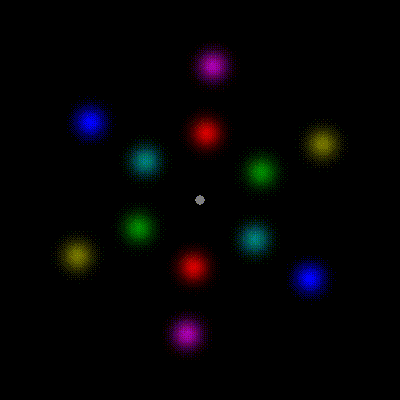
\includegraphics[width=1\linewidth]{movies/LinaresVaziriPashkamHolcombe/pairingOneStimulusCycleSoRotatesPereniallyStatic} \caption{When the discs in this display rotated faster than about 1.4 rps (approximately the 1-target tracking limit with this display), participants were unable to judge whether two colors are adjacent to each other.}\label{fig:spinner}
\end{figure}

An additional result suggested that the spatial relationship is mediated by an attentional shift. When the discs were moving slow enough that participants could often do the task (like in the above movie) but sometimes made errors, the errors had a systematic pattern. The task was to report which disc was aligned with a target disc. Participants tended to err by reporting the trailing disc next to the target rather than the aligned disc, consistent with them making a time-consuming shift of attention from the target, which sometimes landed on the trailing disc because the aligned disc had moved on by the time the attention shift landed \citep{holcombePerceivingSpatialRelations2011}. Based on EEG signals and also eye movement data when the eyes were unconstrained, \citet{franconeriFlexibleVisualProcessing2012} found evidence for an attentional shift when judging the spatial relationship between static stimuli. In a dual-task design, \citet{leeAttentionalCapacityUndifferentiated1999} showed that while several judgments could be made concurrently with an attention-demanding task at the fovea, judgments of the spatial relationship between two stimuli (whether a bisected disk had red on the left or on the right) could not. Finally, using a visual working memory paradigm in which they investigated the effect of set size, exposure duration, and simultaneous versus serial presentation, \citet{smithAttentionweightedSamplesizeModel2016} also found evidence consistent with discrimination of spatial relations involving serial attention.

Because in any one paradigm, serial and parallel processes can yield similar or identical data, a number of experimental manipulations was needed to provide convincing evidence of serial processing for spatial relationships. For example, while visual search results led Treisman to conclude that conjoining two spatially superposed features, such as red with leftward tilted, required a serial process of focused attention \citep{treismanFeatureIntegrationTheory1980}, such results are explainable by limited-capacity parallel processing \citep{palmerAttentionVisualSearch1995}, and the redundant-target paradigm of \citet{thorntonParallelSerialProcesses2007} suggested that no serial process is involved.

\hypertarget{a-case-for-serial-position-sampling}{%
\section{A case for serial position sampling}\label{a-case-for-serial-position-sampling}}

Like for other visual processes, for object tracking we should wait for strong evidence before concluding that tracking involves a serial one-by-one process. Unfortunately, there are some difficulties involved in adapting the paradigms developed for judgments involving static stimuli, so such evidence cannot be obtained by applying the same techniques as were used for spatial relationship judgments.

as we shall see.

Let's clarify exactly what we are interested in here. The question is whether \emph{any} serial process is involved in tracking, because we can already be highly confident that parallel processes are involved. The front end of visual processing, from the retina to primary visual cortex, registering the basic elements of color, form, and motion, clearly operate in massively parallel fashion. The question, then, is whether any process involved in tracking is serial. By ``any process'', I don't mean processes during the response phase, such as clicking on the objects one think are targets, or the daydreaming that may occur while one is also doing the task. Instead, I'm referring to processes that are ordinarily necessary for tracking to be accomplished during the tracking phase of the task.

While the nature of MOT closes off some options for investigating the serial/parallel issue, it does provide a new kind of evidence for serial processing. In particular, after a few assumptions are made, serial sampling makes a specific prediction for the temporal limits on tracking. The most basic assumption is that after a moving target's position is sampled, if its position is not re-sampled before another object takes its place, it will be lost. This is a consequence of the visual system assuming that the objects nearest to the last-recorded positions of the targets are, in fact, the targets. Related to this assumption is that the system does not use motion direction and speed reliably. The evidence that speaks to this is discussed in section \ref{beyondLocation}, but even if it is false, note that violations of this assumption would simply reduce the the size of the effects predicted by the serial account.

For circular trajectories such as those used by \citet{holcombeSplittingAttentionReduces2013}, the product of the speed (in revolutions per second) and number of objects determines how often sampling must be done to avoid losing a target. In an MOT trial with two targets, after one target is sampled, a one-by-one serial process would switch to the other target. If the distractor trailing the target arrives near the first target's former location before the serial process switches back, then we can expect tracking to fail.

Increases in the number of targets reduces how often each individual target is sampled. As a result, the serial switching account predicts a linear relationship between the number of targets and the temporal limit on tracking. In Figure \ref{fig:serialModelFit} below, the predictions are plotted if tracking samples position and switches to another object every 60 ms and every 90 ms.

\begin{figure}
\centering
\includegraphics{tracking-review_files/figure-latex/serialModelFit-1.pdf}
\caption{\label{fig:serialModelFit}The predictions of 60 and 90 ms sampling time are plotted as dashed lines, together with data from Holcombe \& Chen (2013) and Roudaia \& Faubert (2017). The data symbols are horizontally offset to avoid overlap.}
\end{figure}

With every unit increase in the number of targets, the interval between successive samples of that target increases by the sampling time. This is under an optimistic assumption of orderly sampling (the sampling process sampling first one target, then the second target, then the third target, and back to the first target, rather than sampling the second target or third target again); otherwise the predicted slope should be even steeper.

Because a particular sampling time specifies the temporal limits for all target sizes, no parameters needed to be fit here. That is, the dashed lines in Figure \ref{fig:serialModelFit} are not best-fitting regression lines. Their slope and intercept are determined by the sampling time indicated. The lines fit the data fairly well. But how impressed should we be by this? One limitation is that only three target loads were tested, so we should have little confidence that the relationship is truly linear in the way that the model predicts.

An additional issue for interpreting the relationship is that in principle, the temporal limit for covertly tracking a \emph{single} target could be set by a different process than the serial switching hypothesized to set the limit for two and three targets, because with a single target, there is no need to switch attention around. Suprisingly, however, evidence from other paradigms suggests that even when only a single static location is relevant for attention, performance oscillates over time, a pattern which has been dubbed the ``blinking spotlight of attention'' \citep{vanrullenBlinkingSpotlightAttention2007, fiebelkornReportRhythmicSampling2013}.

Thus, we should not really expect the temporal limit for one target to fall on the same line as that for two and for three targets. Yet in the plotted data (Figure \ref{fig:serialModelFit}), it can be seen that the one-target limit may actually fall on the same line. It's as if the sampling interval of attention for a single static location also sets the inter-object sampling interval. While the data are consistent with this, they support this proposition only weakly, because there is considerable statistical uncertainty associated with the data points.

The lower clusters of points on the graph represent the male and predominantly-male datasets. They imply temporal limits, when tracking one target, of between 140 and 200 ms. Recall that because the target must be sampled at twice the temporal limit to avoid confusion with the trailing distractor, one could infer sampling rates from this between 70 and 100 ms. This assumes near-perfect linking of a target's last-sampled position with the nearest neighbor in the new sample, otherwise one should estimate a higher sampling rate. The example dashed lines represent the predictions if sampling occurred at 60 ms (red) and 90 ms (blue) and switching occurred systematically rather than visiting one target twice before sampling the third.

How do these numbers compare to sampling intervals inferred with other paradigms? \citet{macdonaldAttentionalSamplingMultiple2013} studied the continuous wagon-wheel illusion, in which a rotating spoked circle is sometimes perceived to rotate backwards, for which a leading explanation is intermittent sampling \citep{holcombeAreThereCracks2014}. Asking participants to report reversals when they viewed multiple spoked circles, they inferred a sampling interval of 75 ms, which assumes, among other things, that perceived reverse motion is strongest when the wheel travels three-quarters of the inter-spoke angle between samples, yielding a one-quarter backwards rotation with each sample. Their 75 ms figure is similar to what we inferred from tracking. However, \citet{arnoldIllusoryMotionReversals2014} found that the peak frequency for perception of illusory backwards rotation differed for equiluminant motion (5 Hz) and luminance-defined motion (10 Hz in their test), suggesting that results from such experiments cannot be interpreted as providing a constant simple sampling rate for high-level vision.

Studies that use other behavioral paradigms in an attempt to investigate visual sampling suggest sampling intervals longer than 100 ms: 140 ms \citep{reFeatureBasedAttentionSamples2019}, 142 ms \citep{vanrullenBlinkingSpotlightAttention2007}, 130 ms \citep{fiebelkornReportRhythmicSampling2013}, and 140 ms \citep{dugueAttentionSearchesNonuniformly2015}, although the statistics used in some of these studies may have led to spurious findings \citep{brookshireReevaluatingRhythmicAttentional2021}. A visual search study that recorded from neurons in monkeys suggested a 44 ms sampling interval \citep{buschmanSerialCovertShifts2009}. These other studies all used stationary objects or multiple locations that the participant was told to monitor, which conceivably could explain the slower sampling intervals found in some, but there also remains ample reason otherwise for uncertainty.

Despite the sizable and growing neurophysiological and neuroimaging literature on oscillations and intermittent sampling, I have not found a study that tests whether the sampling operates independently in the two hemifields. This is unfortunate given that a hallmark of tracking is its hemifield independence, as reviewed in \ref{twoBrains}.

It might turn out that even after researchers regularly assess whether the sampling they are measuring is hemifield-independent, there will continue to be a large range of rates found. If so, perhaps different tasks result in different sampling rates, and the sampling process can occur more quickly for tracking as it requires sampling position only. Another possibility is that the assumptions underlying the calculations in behavioral studies such as object tracking are wrong. If, for example, motion direction is used to guide the next position sampled, tracking could succeed with a slower sampling interval more similar to those documented in most of the neural studies cited above (but see section \ref{beyondLocation}).

A few studies, while finding evidence for oscillations in some conditions, do not find it to be tied to cued locations in the same way as other papers cited above suggest \citep{werfNoEvidenceRhythmic2021, petersObjectbasedAttentionPrioritizes2020}. The fact that psychology and neuroscience researchers admit to substantial rates of publication bias and p-hacking \citep{jenningsPublicationBiasNeuroimaging2012, johnMeasuringPrevalenceQuestionable2012, rabeloQuestionableResearchPractices2020} raises the spectre of further, unpublished, evidence that is inconsistent with the prevailing narrative of regular oscillations that correspond to an attentional sampling rate.

In summary, despite a wealth of neuroscientific evidence that serial sampling occurs for attentional tasks, which might account nicely for the existence of a coarse temporal limit on tracking, and for its dramatic worsening with target load, more evidence would be needed for this to be strongly supported. And serial sampling is not the only possible explanation of the steep decrease of temporal limit with target load. Conceivably, a parallel process of evidence accumulation with limited capacity could fit the data. Under this account, when attention is split among multiple targets, this greatly slows the rate that of accumulation of evidence for some process that is critical to tracking. This process might be linking successive position samples.

\hypertarget{evidence-for-parallel-processing}{%
\section{Evidence for parallel processing}\label{evidence-for-parallel-processing}}

\citet{howeDistinguishingParallelSerial2010} applied the simultaneous-sequential presentation technique developed by \citet{shiffrinVisualProcessingCapacity1972} to investigate the nature of parallel or serial processing involved in MOT. The technique was developed for tasks involving stationary stimuli and was originally conceived as investigating whether several stimuli could be processed in parallel without being affected by any capacity limit. The stimuli are presented either all at once (simultaneously) or in succession (sequentially) during a trial, half the stimuli presented in the first interval, and the other half in the second interval. To equate the total amount of time each stimulus is presented in the simultaneous and successive conditions, a trial in the simultaneous condition is only half as long as that of the successive condition. The technique has been applied extensively to the detection of a particular alphanumeric character among other alphanumeric characters, and researchers have found that processing in the simultaneous condition is equal to or better than the sequential condition \citep{shiffrinVisualProcessingCapacity1972, hungSimultaneousBetterSequential1995}, suggesting that multiple alphanumeric characters can be recognized in parallel, with no capacity limitation, or at least a capacity that is not taxed by up to the four stimuli typically used. An alternative possibility is that attention for some reason did not select the locations of the presented stimuli during the two intervals of the sequential condition. For example, if attention got ``stuck'' on the locations of the first half of stimuli, it would fail to show the advantage expected for a limited-capacity process that could devote all its resources to each of the two subsets of the stimuli during their respective presentation intervals.

\citet{howeDistinguishingParallelSerial2010} adapted this technique to MOT by, in a ``sequential'' condition, periodically freezing half of the moving targets while the other half continued to move. In the simultaneous condition, \emph{all} of the targets were periodically frozen. The idea, then, is that any parallel processes will be distributed equally among both moving and any temporarily-stationary targets, whereas a serial process must be reallocated away from the stationary targets during the interval that they are stationary. Such a serial process would then result in higher performance in the condition where targets occasionally pause relative to an ``all pause'' condition where all targets are temporarily-stationary at the same time.

Across eight experiments, they found that performance was equal or better in the simultaneous condition than in the sequential condition. They interpreted this result as ruling against a serial model whereby tracking is accomplished by switching a process important for tracking from one (or a few) targets to the others. One assumption of this interpretation is that a serial process should be able to efficiently switch away from targets when they are stationary to selectively process the moving targets. As \citet{howeDistinguishingParallelSerial2010} pointed out, there is good evidence from other MOT experiments that participants can prioritize the most important targets or those perceived to be more difficult to track, for example in virtue of them moving faster \citep{chenResourceDemandsObject2013, croweGoaldirectedUnequalAttention2019}. A concern with the \citet{howeDistinguishingParallelSerial2010} experiments, however, is that the longest non-movement (freeze) interval used in the experiments was half a second, and in most of the experiments, the non-movement interval was only a few hundred milliseconds. It is possible that at that rate, a serial process was unable or ineffective at switching from the stationary targets to the moving targets and back again. In addition, the locations of the targets had to be remembered while they were frozen (to distinguish them from the stationary distractors) so that the serial tracking process could switch back to them. These task requirements for non-moving stimuli is quite different from what was involved in traditional applications of the simultaneous-sequential technique (e.g. \citet{shiffrinVisualProcessingCapacity1972}), where the task was to detect just a single target from among stationary candidate locations.

Regarding the uncertainty around the assumption that a serial process could effectively switch away from the targets when they were stationary during the brief stationary interval, \citet{howeDistinguishingParallelSerial2010} did conduct one experiment that used a longer, 1.5 s interval, for the movement and non-movement phases. However, this study was deliberately designed to favor serial processing, as a kind of sanity check to establish that the technique worked. They presented only two targets and predictably alternated which of them was moving and which was stationary. In contrast to all of their other experiments they found an advantage for the sequential condition, and they concluded that the 1.5 s interval ``was more than sufficient for observers to transfer their attention from one target to another''. But this again raises the question of whether the intervals in the other experiments were simply too short for the serial process to reallocate appropriately. It may be that as one increases the pause interval toward 1.5 s, at some point the sequential condition will show an advantage over the simultaneous condition. What is the criterion for saying what interval is so long that a sequential advantage there no longer speaks to tracking processes? Another issue with this experiment is that because only two targets were used, it likely taps the C≈1 processes more than the previous experiments that used more targets. And, of course, C≈1 processes have a capacity of approximately one, and thus have to process two targets serially.

Returning to the difficult issue of how long of an alternation interval should be used in the simultaneous-sequential design, in a study of word recognition, \citet{scharffExtendingSimultaneoussequentialParadigm2011} used the sequential-simultaneous technique to investigate contrast discrimination and visual word recognition. The contrast discrimination task was to judge which of an array of low-contrast discs had a higher contrast than all the rest (which were all identical in contrast), while the word recognition task was to locate the one word, in a display of words, that belonged to a particular category. For example, in one case the target category was ``animals'', and the word ``dog'' (the target) was present in addition to the words `car,' `belt,' and `poet'. \citet{scharffExtendingSimultaneoussequentialParadigm2011} found no advantage of the sequential condition for judging which of an array of low-contrast discs had a higher contrast, which they interpreted as consistent with parallel, unlimited-capacity processing. In the word recognition task, in contrast, they found a large sequential advantage, which they took as evidence of serial processing. The alternation interval they used was 1.1 seconds, again raising the possibility that \citet{howeDistinguishingParallelSerial2010} might have found a different result with longer intervals, as the longest interval used by \citet{howeDistinguishingParallelSerial2010}, save for in the control experiment, was half a second. In sum, while the \citet{howeDistinguishingParallelSerial2010} evidence might have provided evidence for serial processing and yet did not, a strong possibility remains that in conventional MOT tasks, a serial process rapidly switches among the targets.

\hypertarget{models-of-mot}{%
\section{Models of MOT}\label{models-of-mot}}

In the behavioral studies that revealed the temporal limits on tracking, a target and its distractors all shared the same circular trajectory. But in most studies of MOT, the distractors near a target move in many different different directions relative to the target. That is, typical displays have low trajectory among targets and distractors' trajectories.

All recent models of MOT rely largely on a parallel process for updating of target positions (a serial process is used in some models for other features, which is discussed in \ref{identity}) \citep{oksamaPositionTrackingIdentity2016, lovettSelectionEnablesEnhancement2019, liModelMultipleIdentity2019, oksamaDynamicBindingIdentity2008a, srivastavaAttentionDynamicsMultiple2015, kazanovichOscillatoryNeuralModel2006}. These parallel theories do not seem able to account for the basic temporal limit discovered with circular trajectories and showcased in \ref{speedAndTime}, nor for the temporal limit's dramatic decrease with target load. Most model authors do not mention this issue, and it does not appear that their model can explain the phenomenon \citep{srivastavaAttentionDynamicsMultiple2015, vulExplainingHumanMultiple2010, maNoCapacityLimit2009}. Not only do none of these models predict an increase in temporal interference with target load, most of them never even consider the possibilty of temporal interference.

I am aware of two groups of researchers that have addressed the temporal interference results. \citet{lovettSelectionEnablesEnhancement2019} have a hybrid parallel-serial model of multiple object tracking. Target positions are updated in parallel, but this parallel updating process occurs concurrently with a serial process that, by visiting a target, can utilise the target's features and compute its motion history. By ``motion history'', these researchers seem to mean that the motion direction of the target is processed, which can then be used to predict future positions, which helps disambiguate which is the target and which distractor when objects overlap or come close to overlapping. This helps explain the evidence that localization of targets in such situations can actually be better than targets that are not near distractors \citep{srivastavaAttentionModulatesSpatial2016}. This serial process can thus explain why predictability of motion trajectories yields an advantage when there are only a few targets, but no detectable advantage when there are more \citep{howeMotionInformationSometimes2012, luuExtrapolationOccursMultiple2015}.

To explain the temporal resolution and load results of \citet{holcombeSplittingAttentionReduces2013}, \citet{lovettSelectionEnablesEnhancement2019} deploy their model's serial process in a surprising way. Their idea is that when targets and distractors share circular trajectories as in \citet{holcombeSplittingAttentionReduces2013}, participants shift from parallel tracking to serial tracking, and this results in the decline in temporal frequency limit with load and also the 2 rps speed limit. But unlike for some of their other claims, they never validate this against data by running the model on these trajectories. Moreover, they don't explain how the parallel process contributes to performance during the task. The serial process is needed for circular trajectories, they say, to prevent targets from becoming confused with the trailing distractors that soon occupy the targets' former positions. The model's serial process allows it to predict future positions and was in fact postulated to address overlap situations. This makes some sense, and the serial process is a natural for explaining the approximately-linear decline in temporal limit with load. But presumably the parallel position updating process is still in operation, as it is in other displays that they say involve serial processing, so why would the pattern of performance (a declining temporal limit) be so determined by the serial process?

For a serial process to determine performance in a model where parallel processing ordinarily plays the dominant role in updating target positions, it seems that the parallel process must somehow be disabled. In other words, in conditions where the serial process determines the performance limit, the parallel process' updating of positions must be so inferior that it does not substantially contribute to the pattern of performance. Another way of saying this is that the serial process is the performance-limiting process. This type of reasoning based on the pattern of performance thresholds has long been used in psychophysics \citep[e.g.,][]{victorTemporalPhaseDiscrimination2002}.

Assuming that the limiting process is indeed serial sampling, we can then infer a characteristic of the parallel updating process. The parallel updating process must be effectively updating targets' positions more infrequently than about every 180 milliseconds. That is, if it's true that temporal limit worsens linearly with target load and the serial process determines this performance pattern, implying that the parallel process isn't contributing much, then the parallel process's contribution must be worse than that of the serial process. The 3 Hz limit with 3 targets \citep{holcombeSplittingAttentionReduces2013, roudaiaDifferentEffectsAging2017}, then, places an upper bound on the parallel process' functioning. It is important, then, to measure the temporal limit with 4 targets. This could further delimit the upper bound on the parallel process. And independent of any particular theoretical reasoning, it would be quite remarkable to see the temporal limit on tracking decrease even further to worse than 3 Hz, indeed to close to 2 Hz if the linear trend continued.

\citet{liModelMultipleIdentity2019} have also addressed the effect of load on the temporal limit. Their latest model, MOMIT 2.0, updates the position of targets with a parallel process. To address the temporal limit, \citet{liModelMultipleIdentity2019} wrote that ``when objects move along the same trajectories (e.g., Holcombe \& Chen, 2013) and/or are close to each other, high resolution information is required for discriminating the objects. Thus, tracking becomes more serial''. However, he objects in the Holcombe \& Chen (2013) studies were not close to each other, and I haven't been able to find anything in the description of MOMIT 2.0 that should be hindered by objects sharing a trajectory. Informally, it doesn't feel to me that my attention switches to a different mode with circular trajectories, in displays like \ref{fig:twoTargetsTemporalLimit}. Try it yourself. Of course, it is not necessarily the case that introspection provides any access to parallel versus serial processing.

Given that parallel models can't account for the decline in temporal limit with load, why have they been fairly successful in mimicking human performance with the typical MOT displays not designed to probe the temporal limit? Well, for typical MOT displays, it remains unclear how much temporal interference we should expect - no one has bothered to calculate the distribution of the intervals between targets and distractors visiting a given location. Second, it is not clear how discriminable the models are from the human data. That is, a number of different models might equally well explain the data. One reason is that potential spatial interference and for temporal interference are confounded in typical MOT displays. That is, trials in which the moving objects come close to each other in space also tend to be trials in which moving objects visit approximately the same location in a short span of time. As a result, a model that embodies spatial interference only may explain the data about as well as one that includes temporal interference.

\hypertarget{resolution}{%
\chapter{Serial streak sampling}\label{resolution}}

On the one hand, most theorists have included parallel position updating in their models. This seems to fit the data from MOT experiments with relatively-unconstrained object trajectories quite well - although few have compared the performance of their model with a serial model, so it is hard to know how diagnostic the modeled data are. On the other hand, the data from circular trajectories is hard to explain without positing that serial updating of position dominates. The accounts offered of this dichotomy seem unsatisfactory. However, there is an additional source of information that could assist tracking, one that would disabled by non-circular trajectories.

Long after most researchers considered the idea of serial updating of position to be disproven, Srimant Tripathy and his collaborators made a new case for the idea in a book chapter in 2011 \citep{tripathyMultipleObjectTrackingSerial2011}. Previous researchers had concluded that serial switching of attention would have to occur implausibly rapidly to account for tracking performance \citep{pylyshynTrackingMultipleIndependent1988, yantisMultielementVisualTracking1992, oksamaMultipleObjectTracking2004}. \citet{tripathyMultipleObjectTrackingSerial2011}, however, pointed out that the demands on attention switching would be much less if the tracking process had the benefit of sensory memory traces left by the moving objects, also known as ``motion streaks''. Motion streaks may be familiar from turning on a fan and watching it spin faster and faster until its blades blur perceptually into a complete circle - and in the photograph below, one sees the motion streaks created by a London bus, when photographed with a 200 ms exposure, which is likely comparable to the interval of motion streaks in our visual system.



\begin{figure}

\includegraphics[width=0.8\linewidth]{imagesForRmd/motionBlur/London_bus_and_telephone_box_on_Haymarket} \caption{A London bus, photographed with a 200 ms exposure, by EO1 \href{https://creativecommons.org/licenses/by-sa/2.0/deed.en}{CC BY-SA 2.0}}\label{fig:busMotionBlur}
\end{figure}

At speeds like those used in MOT experiments, the moving objects leave trails of persisting activation in the visual cortex \citep[e.g.][]{apthorpDirectEvidenceEncoding2013}. Consider how the correspondence problem could be solved if the tracking process has access to these motion streaks, c.~Rather than having access to only the most recently-registered position of each object, it would also ``see'' a short trail behind each object. If the rate of position sampling were frequent relative to the duration of visual persistence, then the motion streak would actually connect the last-registered position of an object with the current position sample. In most conditions, this should allow the tracker to avoid many of the confusions between targets and distractors that would otherwise occur. Recall from our explanation of the correspondence problem (\ref{beyondLocation}) that when only discrete positions are sampled, a distractor will be the closest object in the current sample to a target in the previous sample, causing the distractor to be mistakenly taken to be the target.

When motion streaks can be used, either the streak will literally connect the new sample to the old sample, or if the sampling happens less frequently relative to the targets' speed, if the object hasn't changed direction than the streaks will typically be collinear, whereas the distractors' streaks will be positioned and oriented differently. The major exception to this would be when the target shared its trajectory with distractors, such as in the experiments of \citet{holcombeSplittingAttentionReduces2013}.



\begin{figure}
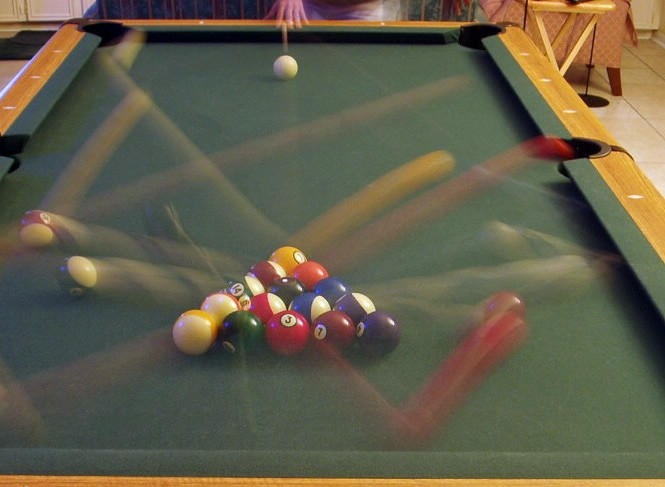
\includegraphics[width=0.8\linewidth]{imagesForRmd/motionBlur/8_ball_break_time_lapsePublicDomain} \caption{The motion streaks created by billiard balls in a long exposure of the ball break \href{https://commons.wikimedia.org/wiki/File:8_ball_break_time_lapse.jpg}{Public domain}}\label{fig:billiardsBlur}
\end{figure}

Step by step, here's how the motion streaks serial sampler could work, in an MOT experiment where the targets and distractors occupy different trajectories. When the sampler visits the last-known position of a target, that position may now be the site of the trailing end of the motion streak, which connects this last-known position of the target to its present position. The tracker can thus follow the streak to arrive at the new target position. The most up-to-date end of the streak is the one with the highest contrast (because it has had the least time to decay). If it has been so long since the sampler visited this target that there is no longer any activation at the last-visited location, there will typically be only a small gap between that location and the trailing end of the target's current streak. The size of that gap will be the distance traveled by the object in the time between samples minus the duration of sensory persistence.

When, as in the \citet{holcombeSplittingAttentionReduces2013} experiments, the target moves about a trajectory that is shared by several distractors, the streaks will be much less helpful. When the serial sampler returns to the last known location of a target, if it does not return before the trailing distractor reaches that location, a new streak will be there, that of the distractor. Thus, this account predicts that in the trajectory-sharing displays, tracking will only succeed if the time between object visits to a location is longer than the time between samples. That is, success at tracking is now limited by serial switching time. This nicely converges with theorists' predilection for proposing a different mechanism for trajectory-sharing displays, even if they have had the wrong idea for why such displays bear the signature of serial switching.

One might be skeptical that motion streaks are available to visual processes such as tracking - after all, we don't usually perceive motion streaks when objects are moving at reasonable speeds. But there is good evidence that motion streaks do affect visual processing. Psychophysical studies have found evidence for perceptual adaptation to the streaks left by moving objects, and also that these streaks mask the visibility of static objects. It has been estimated that these streaks span about 100 ms of a moving object's trajectory, and there is also plenty of physiological evidence for them - see \citet{apthorpSpatialTuningMotion2011} for references. Moreover, recent evidence suggests that the elongated motion streaks created by saccades are used to solve the across-saccade object correspondence problem \citep{schweitzerIntrasaccadicMotionStreaks2020, schweitzerIntrasaccadicMotionStreaks2021}. As for why we don't see motion streaks in many viewing conditions, this is not fully understood, but nearby objects appear to actively suppress their visibility \citep[for a review, see][]{bedellPerceptionMotionSmear2010}.

Tripathy's group conducted a number of studies to investigate the possibility that motion streak information is available. This largely took the form of varying delays between stimulus presentation and cues, showing that participants could report motion direction and detect trajectory changes fairly precisely immediately after objects offset, but that this ability decayed very quickly with time \citep{narasimhanLossPositionalInformation2009, shoonerHighcapacityTransientRetention2010}. The rapid decay was consistent with the time-course of the dissipation of sensory activation, as evident in studies of iconic memory.

In the previous chapter (\ref{serialOrParallel}), when we inferred what the interval between samples needed to successfully track with the circular trajectory displays, we were not considering streaks, so we used the conventional nearest-neighbor interpretation of motion ambiguity, which implies that sampling must occur more frequently than the time it takes for a distractor to move halfway to a former target location \citep{holcombeIllusoryMotionReversal2005}. But motion streaks connect the last-sampled target position to its new position, up until the distractor moves so far that it actually touches the former target location. This is simply the temporal frequency of the stimulus. For example, for the case of three targets where a temporal limit of less than 3 Hz is observed \citep{holcombeSplittingAttentionReduces2013, roudaiaDifferentEffectsAging2017}, we had estimated that samples must occur at least every 167 ms, but motion streaks mean that in principle, the samples need only occur every 332 milliseconds. However, a sizeable gap may be needed to resolve the difference between the front of the motion streak created by the distractor and the trailing end of the motion streak created by the target, so sampling more frequently may be necessary.

\hypertarget{taking-stock}{%
\section{Taking stock}\label{taking-stock}}

When Srimant Tripathy suggested the serial sampling of motion streaks idea, we had not yet discovered the decline with load of tracking's temporal limit. At the time, I did not fully understand Srimant's account, and did not appreciate that the account both predicts this sort of result and also predicts that a quite different result should be found with trajectories that do not highly overlap. It was only when grappling with the suggestion of \citet{lovettSelectionEnablesEnhancement2019} that when distractors and target share trajectories, tracking becomes more serial, that the connection to motion streaks became clear to me. The notion of serial position sampling in tracking converges with the ascendance of evidence for serial sampling in other behavioral and neuroscientific paradigms, and presents a strong prospect for resolving the serial-parallel debate.

The use of motion streaks provides a similar benefit as the use of velocity as a feature for correspondence matching, and studies that investigated the possible use of velocity do not seem to have been designed to discriminate between the use of velocity and the use of motion streaks (e.g., \citet{wangRoleKinematicProperties2021}). One difference is that streaks might provide information only about the orientation of an object's trajectory but not which of the two directions along that orientation the object is moving in. If so, one result should be that participants should more frequently err in the opposite direction that a target is moving than in other directions. It does not appear that studies that collected participants' awareness of direction information checked for this \citep[e.g.][]{shoonerHighcapacityTransientRetention2010, horowitzDirectionInformationMultiple2010}.

\hypertarget{identity}{%
\chapter{Knowing where but not what}\label{identity}}

Consider what someone means when they say they are keeping track of something, for example their family. That likely would mean knowing where each of their siblings is, where their mother is, and where their father is. But the multiple object tracking task does not test peoples' knowledge of the different identities of targets. Rather, the targets are typically all identical to each other (and to the distractors) and people need only report where the targets are.

This section is about what you know about the objects you are tracking. The broad answer is: surprisingly little. We should break the question down, however, into two questions. A first question is about how position updating works - does it use differences between the distractors' and targets' features to help keep track of the targets? A second question is about the extent to which targets' features are available to conscious awareness.

\hypertarget{the-first-question-does-position-updating-benefit-from-differences-in-object-identities}{%
\section{The first question: Does position updating benefit from differences in object identities?}\label{the-first-question-does-position-updating-benefit-from-differences-in-object-identities}}

\hypertarget{motion-correspondence}{%
\subsection{Motion correspondence}\label{motion-correspondence}}

Computer algorithms have been developed for object tracking to facilitate detection of intrusions and safety threats in industrial settings. They are also used for analyzing the movements of players of an opposing team's previous games as well as the movements of animals in lab experiments. When developing tracking algorithms, engineers do not confine themselves to using only the locations and motions of objects - they also use the appearance of those objects, for example their shapes and colors. This helps the algorithm match objects across video frames (the correspondence problem, sometimes known as the ``data association problem'' in engineering) \citep{yilmazObjectTrackingSurvey2006a}. This allows successful tracking in situations where location and motion alone would result in losing a target.

Of course, the fact that object features would be useful for the brain to use for tracking does not necessarily mean that the brain does use them. One aspect of the architecture of the brain suggests that it might not. Famously, as visual signals leave the occipital cortex, visual processing divides into two streams, ventral and dorsal. The dorsal stream, sometimes called the ``where'' pathway, specializes in motion and position processing, while the ventral stream, the ``what'' pathway, specializes in object recognition \citep{goodaleSeparateVisualPathways1992}. While the pathways do interact, this division raises the possibility that position updating might not involve much processing of objects' features.

Beginning over a century ago, Gestalt psychologists such as Max Wertheimer found that apparent motion was equally strong whether the objects in successive frames were identical or different \citep{wertheimerExperimentelleStudienUber1912}. Later studies found some effect of similarity, but the effect was weak \citep{kolersFiguralChangeApparent1971, burtTimeDistanceFeature1981}. These findings contributed to the dominant view that the visual system does not use feature similarity much when computing motion correspondence to update a moving object's position. Some caution is justified, however, because
when the successive presented frames of an object touch or overlap with each other rather than being presented in non-contiguous locations, the results can be different. The study of such displays, with a different object appearance (usually, shape) in two successive frames, is known as line motion or transformational apparent motion. These studies have found that feature similarity, especially contour continuity, but also color, can decide which tokens are matched \citep{faubertInfluenceTwoSpatially1995, tseRoleParsingHighlevel1998}. Thus, feature similarity is involved in motion processing, even though in many situations motion correspondence is determined by spatiotemporal luminance relationships. An important characteristic of this process that does does not seem to have been studied, however, is whether these cues are processed in parallel. Short-range spatiotemporal luminance relationships (``motion energy'') are known to be processed by local detectors, such that visual search happens in parallel for a target moving in an odd direction defined by small-displacement apparent motion \citep{horowitzAttentionApparentMotion1994}. I am not aware of any studies that have investigated this for transformational apparent motion, in a situation where the perceived motion direction is determined by feature similarity. Thus, the possibility remains that feature similarity has its influence through what I have called a C\textasciitilde1 process.

\hypertarget{feature-differences-but-not-feature-conjunction-differences-benefit-tracking}{%
\subsection{Feature differences, but not feature conjunction differences, benefit tracking}\label{feature-differences-but-not-feature-conjunction-differences-benefit-tracking}}

Another way that object identity information might benefit position tracking is via the action of feature attention. A clear case is if the targets differ in color from the distractors. It is well-established that attention can select stimulus representations by their color. One can, for example, enhance the selection of all red objects in the visual field. \citet{makovskiFeatureBindingAttentive2009} confirmed that this process can benefit MOT. They used eight moving objects, four of which were targets. MOT performance was better than when the eight objects were different in color than when they were identical. This was also true whe the objects were each a different shape.

A large body of evidence from other paradigms has supported the theory of \citet{treismanFeatureIntegrationTheory1980} that feature pairing information, in contrast to individual features, cannot efficiently guide attention to targets. If the splitting of attention among multiple locations that occurs in MOT is similar to how attention is diffused over multiple stimuli in visual search and other paradigms, then one would expect that targets having unique feature pairings would not benefit tracking performance. \citet{makovskiFeatureBindingAttentive2009} found good evidence for this. In their ``feature conjunction'' condition, each object had a unique pair of features, while it shared the individual features with at least one other object. Performance was no better in this condition than if the objects were all identical.

\hypertarget{the-second-question-are-we-aware-of-the-identities-of-objects-we-are-tracking}{%
\section{The second question: Are we aware of the identities of objects we are tracking?}\label{the-second-question-are-we-aware-of-the-identities-of-objects-we-are-tracking}}

We are of course aware of object features when the only task we are engaged in is tracking a single target. In that situation, our limited-capacity processes can all be applied to that target. However, when we are tracking multiple targets, the evidence indicates that we have little ability to report the objects' features, other than their locations, as we will see below.

A common view among the public is that lack of awareness of the features of objects one is attending to could not happen. Indeed, many people seem to believe that we are simultaneously aware of the identities of all the objects in the central portion of our visual field, so unless an object actually disappears or hides behind something or someone, we should know where everything in the scene is at all times, and we should immediately detect any changes to these objects. For many, change blindness demonstrations are the first experience that disrupts this belief.

Experiments suggest that during change blindness, although people cannot monitor a large number of objects at once, they are able to monitor several, perhaps four or five \citep{rensinkVisualSearchChange2000}. They appear to do this by loading the objects into working memory and then, in the second frame, checking whether any are different than what is held in memory. A vast literature on visual working memory has confirmed that people can store several objects and rapidly compare these stored representations to the visual scene. However, loading into memory the features of objects for storage and subsequent comparison is not the same as maintaining awareness of the changing features of such objects. For one thing, it appears that hundreds of milliseconds are needed to encode several objects \citep{vogelTimeCourseConsolidation2006, ngiamVisualWorkingMemory2019}. Second, it appears that when objects are in motion, updating of their features is particularly poor, as we will see in the next section.

When Zenon Pylyshyn published the first theory of multiple object tracking, he had already devised the concept of FINSTs (Fingers of Instantiation), a small set of discrete pointers allocated to tracked targets. The idea was that each discrete pointer allows other mental processes to individuate and link up with an object representation, with the continued assignment of a pointer to a target facilitating its representation an object's representation as the same persisting individual \citep{pylyshynRoleLocationIndexes1989}.

Pylyshyn's theory implied that when tracking multiple targets, people should know which target is which. To his credit, Pylyshyn tested this and other predictions of his theory, and when the results turned out differently than expected, he published his results, in two papers. The first paper was entitled ``Some puzzling findings in multiple object tracking: I. Tracking without keeping track of object identities''. In one study in that paper, targets were assigned identities either by giving them names or by giving them distinct and recognizable starting positions: the four corners of the screen \citep{pylyshynPuzzlingFindingsMultiple2004}. At the end of a trial, participants had the usual task of indicating which objects were targets, but also were asked about the identity of the target - which one it was. Accuracy at identifying the targets was very low, even when accuracy reporting their positions was high.

More evidence for a disconnect between knowledge of what one is tracking and success at the basic MOT task was found by \citet{horowitzTrackingUniqueObjects2007}, who had participants track targets with unique appearances - in one set of experiments, they were cartoon animals. At the end of a trial, all the targets moved behind occluders so that their identities were no longer visible. Participants were asked where a particular target (say, the rabbit) had gone - that is, which occluder it was hiding behind. This type of task was dubbed ``multiple identity tracking'' by \citet{oksamaMultipleObjectTracking2004}. Performance was better than chance, but was much worse than performance for reporting the target locations irrespective of which target it was. The effective number of objects tracked, as reflected in a standard MOT question, was about four, but when asked to indicate the final location of a particular animal, capacity was estimated as closer to two objects.

These results of MIT experiments suggest that our ability to update the location of objects of interest is much better than our ability to maintain knowledge of what those objects are. This harkens back to Pylyshyn's original idea that tracking is mediated by pointers that in and of themselves, only point to locations and don't contain other featural information. Pylyshyn thought that these pointers, being unique and distinct, did provide us with knowledge of which target location at the end of a trial corresponded to a particular target at the beginning of a trial. However, his own experiments ruled against that - the tracking process seems to deploy something to the moving targets that carries absolutely no information about those targets other than their positions.

Given enough time, we certainly can update our representation of not only the locations of targets but of their features. For example, in visual short-term memory experiments, on successive trials people memorize different location-feature mappings for several objects. Thus, if moving objects were simply to move very, very slowly, we should be able to update our awareness of what is where before any target travels more than a trivial distance. However, a quite recent study yielded some results that further showcase the limitations of our identity updating abilities.

\hypertarget{beaten-by-a-bird-brain}{%
\section{Beaten by a bird brain}\label{beaten-by-a-bird-brain}}

\citet{pailianAgeSpeciesComparisons2020} conducted a test that at an abstract level, was similar to Pylyshyn's experiments, with identical objects assigned unique identities. \citet{pailianAgeSpeciesComparisons2020}, however, used a format much like the ``shell game'' utilised by magicians and hustlers for hundreds of years. The engaging nature of the shell game format made it suitable for testing children and an African grey parrot as well as human adults. This led to a few surprises.

For stimuli, \citet{pailianAgeSpeciesComparisons2020} used colored balls of wool. Between one and four of the balls were shown to a participant. The experimenter covered the balls with inverted opaque plastic cups, and then began to move them, swapping the positions of one pair at a time. After a variable number of pairs were swapped, the experimenter presented another ball with one of the target colors, and the participant's task was to point to (or peck on!), the cup containing the probed color.

\begin{figure}
\centering
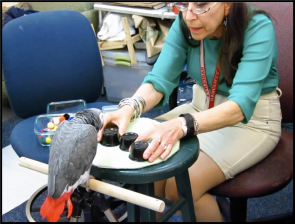
\includegraphics[width=0.4\textwidth,height=\textheight]{imagesForRmd/ParrotGriffinPepperbergShellGame.png}
\caption{An African grey parrot participates in a shell game. CC-BY Pailian et al.~(2020)}
\end{figure}

At any one time, only two objects were in motion, and that the participants were responsible for knowing the final location of all the colors - there were no distractors. One might anticipate that at least the adults would be able to perform this task with high accuracy, especially given that at any one time, only two objects were in motion and the experimenter paused for a full second between swaps, which ought to give people enough time to update their memory of the locations of those two colors.

When only two balls were used, over 95\% accuracy was seen even for four swaps, the highest number tested. This was true of all three participant types: the children, the parrot, and the human adults. In the three-ball condition, for the children, who were 6 to 8 years old, performance was still near ceiling for the zero-swap (no movement) condition, but fell to close to 80\% correct in the one-swap condition, and fell to around 70\% correct for two and three swaps. The adults did better, but still their performance fell with number of swaps, to about 80\% correct for four swaps. Remarkably, the parrot actually outperformed not only the children, but also the human adults. Importantly, the parrot had not been trained extensively on the task, learning it primarily by simply viewing the experimenter and a confederate perform three example trials (the parrot was experienced with a simpler version of the task involving only one object presented under one of the three cups).

The biggest surprise here is that an African gray parrot had the ability to remember and update small sets of moving hidden objects to a level of accuracy similar to humans, despite having a much smaller brain than ours, less than one-fiftieth the size of our own in fact. Because large parts of the parrot brain evolved after they split from our lineage \citep{iwaniukInterspecificAllometryBrain2005}, the existence of this ability in its brain looks to be an example of convergent evolution.

A second surprise was that the adult humans (in this case, Harvard undergraduates, who surely had high intelligence on average) displayed levels of accuracy that was not very high for the conditions that involved more than a few swaps. Remember that in these experiments, only two balls were moved at a time, and there was a one-second pause between swaps. Prior to the publication of this study, I had assumed that the reason for poor performance in multiple identity tracking was the difficulty of updating the identity of three or four targets while they moved. I would have predicted that changing positions exclusively by swapping the positions of two objects, and providing a one-second pause between swaps, would lead to very high performance. The \citet{pailianAgeSpeciesComparisons2020} results suggest that updating the memory of object locations is very demanding.

This finding was also surprising based on the long-accepted concept of ``object files'' developed by \citet{kahnemanReviewingObjectFiles1992}. The idea was that all the features of an object are associated with a representation in memory, the object file, that is maintained even as the object moves. \citet{kahnemanReviewingObjectFiles1992} showed a preview display with two rectangles, with a feature (in most experiments, a letter) presented in each. The featural information disappears, and then the rectangles would move to a new location. The observer's representation of the display is then probed, for example by presenting a letter again in one of the rectangles and asking participants to identify it. \citet{kahnemanReviewingObjectFiles1992}
found that if the letter was the same as the one presented in that rectangle at the beginning of the display, observers were faster to respond than if it had appeared in another rectangle in the beginning of the display, indicating that that aspect of the rectangle's initial properties was maintained, with its location updated. The focus in these studies was on simply demonstrating that this response time priming occurred at all, not in assessing what proportion of time it occurred.

Many researchers may have made the same mistake that I did of assuming that several object files could easily be maintained and updated. However, even in the original experiments of \citet{kahnemanReviewingObjectFiles1992}, they found that the amount of priming was greatly diminished when four letters were initially presented in different rectangles, indicating that fewer objects than that had letter information maintained and updated. They concluded that there may be a severe capacity limit on object files. This was also supported by a pioneering study by \citet{saikiMultipleobjectPermanenceTracking2002}, who had participants view a circular array of colored discs that rotated about the center of the screen. Occasionally discs swapped color when they briefly went behind occluders, and the participants' task was to detect these color switches. Performance decreased dramatically with speed and number of discs, even though the motion was completely predictable, and \citet{saikiMultipleobjectPermanenceTracking2002} concluded that ``even completely predictable motion severely reduces our capacity of object representations, from four to only one or two.'' Bcause we now understand that simple MOT does not work well across occluders, however, that interpretation of the study is limited by the absence of an MOT-type control. Nevertheless, the evidence from the studies in this chapter overall suggests that identity updating is very poor in a range of circumstances.

\hypertarget{some-dissociations-between-identity-and-location-processing-reflect-poor-visibility-in-the-periphery}{%
\section{Some dissociations between identity and location processing reflect poor visibility in the periphery}\label{some-dissociations-between-identity-and-location-processing-reflect-poor-visibility-in-the-periphery}}

If it is the case that participants cannot update the identities of the moving objects that they are tracking nearly as well as they can update their positions, why is that? The results of an eye tracking study by the Finnish researchers Lauri Oksama and Jukka Hyönä led them to conclude that identities are updated by a serial one-by-one process. Eye movements during MOT were contrasted with those during MIT, in which the targets and distractors were line drawings. During MIT, participants looked directly at targets frequently, totalling around 50\% of the trial duration, and frequently moved their eyes from one target to another. In contrast, during MOT, the participants moved their eyes infrequently, and their gaze wasn't usually at any of the moving objects, rather they were usually looking somewhere close to the center of the screen. \citet{oksamaPositionTrackingIdentity2016} took these results to mean that the targets' identity-location bindings that must be updated during MIT are updated by a serial one-by-one process, whereas target positions during MOT are updated by a parallel process.

What \citet{oksamaPositionTrackingIdentity2016} did not address is that limitations on human peripheral vision mean that participants may have had to update target identity information one-by-one. That is, the targets, line drawings of different objects, likely were difficult to identify when in the periphery. Thus, participants had to move their eyes to each object to refresh their representation of which was which. Indeed, in a subsequent study \citet{liModelMultipleIdentity2019} tested discriminability of the objects in the periphery and found that accuracy was poor.
When they instead used colored discs as stimuli, accuracy was higher in the periphery and participants did not move their eyes as often to individual targets. This suggested at least some degree of parallel processing, leaving the amount of serial processing, if any, in doubt.

In summary, many findings of differences between MIT and MOT performance may be explained by poor recognition of the targets in the periphery. Because most studies of MIT do not include an assessment of how recognizable their stimuli are in the periphery (\citet{liModelMultipleIdentity2019} is the only study I know of that did this), it is hard to say how much of the difference between MIT and MOT can be attributed to this. I am not sure how one would equate object localization with object identifiability; the old apples and oranges problem. One could blur the objects to impair localization but it is not clear what degree of spatial uncertainty is comparable to a particular level of object identifiability.

One dissociation between identity and location tracking performance seems to remain valid regardless of the difficulty of perceiving object identities in the periphery. This is the original finding by \citet{pylyshynRoleLocationIndexes1989}, which was replicated by \citet{cohenWhatwhereTradeoffMultipleidentity2011} that if targets are actually identical but are assigned different nominal identities, participants are very poor at knowing which is which at the end of the trial. Because in this paradigm, there is no visible identity information and participants knew this, the resolution of the periphery was not an issue.

\hypertarget{evidence-from-two-techniques-suggests-parallel-updating-of-identities}{%
\section{Evidence from two techniques suggests parallel updating of identities}\label{evidence-from-two-techniques-suggests-parallel-updating-of-identities}}

\citet{howeIdentityLocationBindingProblem2015a} used two techniques to investigate the possibility that serial processes are involved in multiple identity tracking. First, Howe et al.~applied the simultaneous-sequential presentation technique that they previously applied to MOT,
as discussed in \ref{serialOrParallel}. For the MIT task, four targets of different colors moved among four distractors. Each of the four distractors was the same color as one of the targets, so that the targets could not be distinguished from the distractors by color. In the simultaneous condition, all the objects moved for 500 ms and then paused for 500 ms, with this cycle repeating throughout the length of the trial (which varied randomly between 8 and 16 s). In the sequential condition, half the targets moved for 500 ms while the other half were stationary, and subsequently the other half of targets moved for 500 ms while the others remained stationary. This cycle repeated throughout the length of the trial. In two different versions of the experiment, performance was similar in the simultaneous and sequential conditions, supporting the conclusion that there was no serial process involved in multiple identity tracking. However, the \citet{howeIdentityLocationBindingProblem2015a} conclusion is limited by its assumption that any serial process could respond efficiently to the pause in half the targets by shifting its resources to the moving targets, while not causing any forgetting of the locations and identities of the temporarily-stationary targets. To support this assumption, \citet{howeIdentityLocationBindingProblem2015a} pointed out that \citet{hogendoornTimeCourseAttentive2007} had shown that attention could move at much faster rates than 500 ms per shift. However, the \citet{hogendoornTimeCourseAttentive2007} did not assess the attention shifting time between unrelated targets, rather their shifts were for attention stepping along with a single target disc as it moved about a circular array. Thus, it is unclear to what extent the results of \citet{howeIdentityLocationBindingProblem2015a} undermine the serial, one-by-one identity updating idea embedded in the theories of Oksama \& Hyönä and \citet{lovettSelectionEnablesEnhancement2019}.

\citet{howeIdentityLocationBindingProblem2015a} further investigated serial versus parallel processing in MIT by using a completely different technique: the systems factorial technology of Jim Townsend and colleagues \citep{townsendSerialVsParallel1990}. Two targets were designated for tracking and presented in the same hemifield, to avoid independence by virtue of the hemispheres' independence \citep{alvarezIndependentResourcesAttentional2005}. The participants were told to monitor both targets as they moved and that if either of them darkened, to press the response button as quickly as possible, after which all the disks stopped moving and the participant was asked to identify the location of a particular target, for example the green one (the objects were identical during the movement phase of the trial but initially each was shown in a particular color). To ensure that participants performed the identity tracking task as well, only trials in which the participant reported the target identity correctly were included in the subsequent analysis. Performance detecting the darkening events was very high, at 95\% correct. On different trials, either both targets darkened, one of them darkened, or neither of them darkened, and each could darken either by a small amount or by a large amount. The pattern of the distributions of response time for the various conditions ruled out serial processing (under certain assumptions) and implicated limited-capacity parallel processing. This suggests that participants can process luminance changes of two moving targets in parallel while also maintaining knowledge of the identity of the moving targets. One reservation is that it is unclear how often the participants needed to update the target locations and refresh their identities, because the rate at which they needed to be sampled to solve the correspondence problem is unclear for the particular trajectories used. It also would be good to see these techniques applied to targets defined only by distinct feature conjunctions, with no differences in features between the targets and the distractors. Because this would prevent any contribution of feature attention, and because processing of feature pairs may be more limited-capacity than that of identifying individual features, the results might provide less evidence for parallel processing.

\hypertarget{eye-movements-can-add-a-serial-component-to-tracking}{%
\section{Eye movements can add a serial component to tracking}\label{eye-movements-can-add-a-serial-component-to-tracking}}

Partially in response to the evidence of \citet{howeIdentityLocationBindingProblem2015a} against serial processing in tracking, Oksama and Hyona, with their Chinese colleague Jie Li, revised their Model of Multiple Identity Tracking (MOMIT) to involve more parallel processing. Specifically, MOMIT 2.0 proposes that the ``outputs of parallel processing are not non-indexed locations but proto-objects that contain both location and basic featural information, which can be sufficient for tracking in case no detailed information is required'' \citep{liModelMultipleIdentity2019}. This is a reasonable response to the evidence, even if it unfortunately means the theory doesn't make as strong predictions, as the role of serial processing is now more vague. In MOMIT 2.0, serial processing is tied to eye movements and is used to acquire detailed visual information for refreshing working memory representations. This ``prevents the resolution of the active representations from declining. This is vital for tracking targets that require high-resolution information to be identified and kept distinguishable from other targets.'' The theory seems to be mute on whether serial processing would be involved if both fixation were enforced and the stimuli were easily identifiable in the periphery.

Here it is sensible to step back and consider the overall role of eye movements in ecological task behavior. People move their eyes on average three times a second, in part because like many other animals, our retina has a specialized part (the fovea) that is adaptive to direct at whatever object we are most interested in at the moment. In natural tasks, it may be rarely the case that all the visual signals of interest are clustered together enough that they can be processed adequately without eye movements. Moreover, animals such as ourselves have strong drives for exploration and vigilance because we evolved in changing environments about which we had only partial knowledge.

Eye movements normally contribute a serial, one-by-one component to processing, because as \citet{liModelMultipleIdentity2019} highlighted, very high-quality information comes from only a single region on the screen - the region currently falling on the fovea. Near-continual scanning of the visual scene is a deeply ingrained habit, and extends to artificial tasks like reading. Not only are saccades frequent during reading, but one influential theory of reading proposes that an internal rhythm drives saccades from one word to the next rather than them being triggered by the completion of a process such as word recognition \citep{engbertDynamicalModelSaccade2002}. Perhaps, then, one should expect frequent eye movements to occur and contribute a serial component of processing to a range of tasks even when such eye movements are not necessary. People are also cognitively ``lazy'' in that they seem to structure eye movements and other actions in tasks so as to minimize short term memory requirements \citep{hayhoeTaskConstraintsVisual1998}. Thus, even if saccading to different targets were inefficient, people may do it anyway.

To move the debate regarding the role of serial and parallel processing forward, we should recognize that the frequent eye movements associated with natural behavior should be expected in tracking, as for any task involving multiple relevant stimuli, and this can contribute a serial processing component, even if people can perform the same task in a much more parallel fashion when eye movements are constrained. The most interesting evidence for serial processing, then, may be that found when eye movements are prohibited. This is one reason that the steep decrease in apparent sampling frequency discovered by \citet{holcombeSplittingAttentionReduces2013} (see section \ref{serialOrParallel}) may be very important.

In summary, there is plenty of evidence that both use of object identities in tracking and the updating of target identities for awareness is quite poor. This fits with a much broader set of findings over the last thirty years, that the mind maintains fewer explicit visual representations than we intuitively believe. The first findings of change blindness, which were in the context of failures to detect changes that occurred during eye movements \citep{mcconkieRoleControlEye1979}, led \citet{oreganSolvingRealMysteries1992a} to suggest that ``the world is an outside memory'' and to discover change blindness \citep{rensinkSeeNotSee1997}. The idea was that the impression that one has a rich representation of all the objects in the visual field is an illusion, and instead that one has only a more limited knowledge, but that this is quickly supplemented by attentional processing when one becomes interested in a particular location or object. It appears that O'Regan's big idea goes further than he anticipated. While O'Regan suggested that only when objects were attended would they be fully processed, he did not suggest that one might be able to track the changing locations of multiple targets without becoming aware of what they are. Such lack of awareness has been documented not only in the context of tracking multiple objects as reviewed above, but even in a change blindness task that involved eyetracking of just a single target as part of an ongoing, more complex task \citep{trieschWhatYouSee2003}.

\hypertarget{abilities}{%
\chapter{Abilities and individual differences}\label{abilities}}

There are two basic approaches to understanding the abilities that underlie multiple object tracking. One is the classic experimental approach of dissociating the processes involved by manipulating different factors within participants. This has been the dominant approach and has led to our present understanding of the roles of spatial interference, temporal interference, and the duration that one can sustain attention. However, a small but growing literature has used the complementary individual-differences approach. In the individual-differences approach, the pattern of variation in scores on multiple tests is examined to see which abilities tend to go together. Those abilities that co-vary the most are thought to likely share more processes in common than those that don't.

\hypertarget{do-people-vary-much-in-how-many-objects-they-can-track}{%
\section{Do people vary much in how many objects they can track?}\label{do-people-vary-much-in-how-many-objects-they-can-track}}

There are two very common pitfalls of individual-difference studies in this literature. These are in addition to the common mistake across all study types of not testing enough participants to have good statistical power - individual-difference studies can require more than ten times as many participants as a within-participants experimental design investigating a large effect \citep{schonbrodtWhatSampleSize2013}.

\citet{meyerhoffIndividualDifferencesVisual2020} tested fifty participants and for each one calculated the effective number of items tracked, for a display with four targets and four distractors, the modal effective number of items tracked was around two, but a substantial proportion of participants came in at three targets or one target tracked, and a few scored close to zero items tracked. It is tempting to conclude, as \citet{meyerhoffIndividualDifferencesVisual2020} did, that some participants could only track one or zero targets, while others can track more. Unfortunately, in the data of \citet{meyerhoffIndividualDifferencesVisual2020}, like that of many others, there is no way to know how much of the variation between individuals is due to motivation rather than ability. Measuring motivation reliably is difficult or impossible, so this is not something that can easily be remedied. But researchers can include what are sometimes called attention checks or catch trials to allow exclusion of participants who show clear evidence of not reading the instructions carefully or frequently not paying attention. This is the first pitfall, failing to include some sort of measure that checks whether each participant is blowing off the task.

\citet{oksamaMultipleObjectTracking2004} were also interested in how many objects people can track with reasonable accuracy. They made the effort to test 201 participants, and like \citet{meyerhoffIndividualDifferencesVisual2020} they found what appeared to be a substantial variation in capacity, with some people able to track six objects, while many could track only two or even just one. However, no analyses were reported regarding the reliability of the MOT test. Their participants, who were provided by an air pilot recruitment program, were made up entirely of those who scored in the top 11\% on intelligence test scores from a larger group. This provides some confidence that the participants were motivated, although it is not clear that the intelligence tests were administered in the same session, so one cannot know whether the participants were motivated during this particular session.

While we can be fairly confident that \citet{oksamaMultipleObjectTracking2004} used motivated paticipants, the study suffers from what I refer to as the second pitfall - the failure to assess task reliability. On any test, a participant will tend to get somewhat different scores when tested on two different occasions, even if they did not learn anything from their first experience with the test. The extent to which participants' scores are similar when taking a test twice is known as test-retest reliability. Ideally, this is measured with two tests administered at very different times, but a more limited measure is provided by dividing a single session's trials into two groups and calculating the correlation between those two groups, which is known as split-half reliability. Knowing the reliability can allow us to calculate how much of the variation in scores between participants is expected based on the noisiness of the test. Without knowing the reliability, there remains the possibility that the extreme variation in scores, with some participants' data indicating that they could only track one target, could be due to limited reliability - extensive testing of these participants might reveal that their low score was merely a fluke.

Subsequent studies, fortunately, have assessed reliability, albeit only with the split-half measure rather than on separate days. Still, the reliabilities they have found for MOT are extremely impressive - 0.96 \citep{huangMeasuringInterrelationsMultiple2012}, 0.85 \citep{wilbiksIndividualDifferencesMultiple2020}, 0.92 \citep{trevinoBridgingCognitiveNeuropsychological2021}, and 0.87 \citep{eayrsEstablishingIndividualDifferences2018}. Most other attentional and cognitive tasks have lower reliablities, indeed many basic cognitive and attentional tasks have notoriously low reliabilities \citep{hedgeReliabilityParadoxWhy2018}, and indeed, in these papers, MOT consistently scored near the top of the tests administered. Tasks with low reliabilities are not well suited for individual-differences studies - as mentioned above, individual-difference studies are largely based on measuring the pattern of correlations between tasks to reveal the relationship among abilities. The lower the reliability of a task, the harder it is to reliably measure the correlation with another task.

What do these high reliabilities mean for tracking? It suggests that the large individual differences observed by \citet{oksamaMultipleObjectTracking2004} and others are actually real. It seems that some young, healthy, high-intelligence people can only track one target. Second, it means that individual-difference studies should be an excellent avenue for gaining new insights about tracking and its relation to other mental abilities.

Ageing is likely a major source of individual differences, as older participants perform much worse than younger participants \citep{trickAgerelatedDifferencesMultipleobject2005, sekulerAgerelatedChangesAttentional2008, roudaiaDifferentEffectsAging2017}. Using a task requiring participants to detect which of multiple objects had changed its trajectory, \citet{kennedyEarlyAgerelatedDecline2009} found a steep decline between 30 and 60 years, where the effective numbers of tracked trajectories during Tripathy's multiple trajectory tracking task dropped by about 20\% with each decade of aging, which could not be explained by a drop in visual acuity. This is interesting in itself, and is something that theories of aging and attention ought to explain, but I can't say more as I know very little about aging. This result must also color our interpretation of individual-difference studies using samples with a wide age range --- some of the correlations with other tasks will likely be due to those abilities declining together rather than them being linked in people of the same age. That's still useful for drawing inferences, but slightly different inferences.

Researchers have taken what one might call a wide-angle approach to MOT individual difference studies. They've tested participants with a wide variety of tests, to see which mental abilities are linked. However, the first large-scale study concentrated on tasks typicaly thought of as attentional \citep{huangMeasuringInterrelationsMultiple2012}. Liqiang Huang and his colleagues used tests tof conjunction search, configuration search, counting, feature access, spatial pattern, response selection, visual short-term memory, change blindness, Raven's test of intelligence, visual marking, attentional capture, consonance-driven orienting, inhibition of return, task switching, mental rotation, and Stroop. Administered to a sample of Chinese university students (age not reported, but presumably mostly young adults), many of these tasks showed high reliabilities of over 0.9, meaning that there was a potential for high inter-task correlations (inter-task correlations are limited by the reliabilities of the two tasks involved). However, the highest correlation of a task with MOT was 0.4. The task was counting, which required judging whether the number of dots in a brief (400 ms) display were odd or even. Change blindness, feature access, visual working memory, and visual marking were runner ups with correlations of around 0.3.

That no task had a higher correlation is very interesting, but also disappointing. It's interesting because it suggests that MOT involves distinct abilities from several other tasks that on various grounds have been lumped together with MOT as all being ``attentional''. This is disappointing first because it suggests that our theoretical understanding of these tasks is sorely lacking. It's also disappointing because the low correlations mean that it's hard to discern the pattern of correlations, e.g.~from most correlated to least correlated with MOT - when the highest correlations is 0.4, one needs very narrow confidence intervals to be confident of the ordering of the tasks.

\citet{trevinoBridgingCognitiveNeuropsychological2021} reported data from more than 400 participants tested online, an opportunity sample with a very wide range of ages, from 18 to 89. They tested a set of cognitive, attentional, and common neuropsychological tasks: arithmetic word problems, the trial-making task, digit span, digit symbol coding, letter cancellation, spatial span, approximate number sense, flanker interference, gradual onset continuous performance, spatial configuration visual search, and visual working memory as well as MOT. MOT had among the highest reliabilities, at 0.92. MOT performance had little correlation with performance on the task designed to measure sustained attention over an extended period (about five minutes, the gradual-onset continual performance task \citep{fortenbaughSustainedAttentionLife2015}. This supports the tentative conclusion, already suggested in Chapter \ref{whichAspects}, that the ability to sustain attention without lapses is not an important determinant of tracking performance (as was ).

In the \citet{trevinoBridgingCognitiveNeuropsychological2021} inventory, the task that most resembled the counting task of \citet{huangMeasuringInterrelationsMultiple2012}, which \citet{huangMeasuringInterrelationsMultiple2012} found had a high correlation with MOT, was the approximate number sense task, with a moderate correlation of 0.3. It differed from the counting task of \citet{huangMeasuringInterrelationsMultiple2012} by not testing the subitizing (less than 5 items) range, which might help explain any discrepancy. In a more limited study, \citet{eayrsEstablishingIndividualDifferences2018} found, using hierarchical regression, that subitizing made a contribution to predicting MOT performance that was somewhat separate to that of an estimation task using larger set sizes.

The tasks with the highest correlations with MOT in the data of \citet{trevinoBridgingCognitiveNeuropsychological2021} were visual working memory, spatial span, letter cancellation, and digit symbol coding, all at around 0.5. As the authors pointed out, the letter cancellation and digit symbol coding tasks are complex tasks developed in neuropsychology that are believed to reflect a number of abilities. This makes it hard to interpret their correlation with MOT. Spatial span and visual working memory are quite different from MOT, but similar to each other in that they both involve short-term memory for multiple visual stimuli.

Overall, there is a reasonable level of agreement across these individual-differences studies, as well as others not described here, such as \citet{trickSpatialVisuospatialWorking2012}. They agree that visual working memory has a robust correlation with MOT performance, which is particularly interesting because superficially, MOT imposes little to no memory demand. Most researchers conceive of tracking as involving allocating multifocal attention to multiple targets simultaneously, with a process autonomous to memory causing the foci of attention to move along with the moving targets.

From the consistently strong correlation of MOT performance with visual working memory, it is tempting to conclude that mechanistically the two tasks are tightly linked. However, it must be remembered that working memory tasks are among the best predictors of a wide range of tasks, including intelligence as well as the Stroop task, spatial cuing, and task switching \citep[e.g.][]{redickWorkingMemoryCapacity2006}.

\hypertarget{going-deeper}{%
\section{Going deeper}\label{going-deeper}}

Variation in multiple object tracking is unlikely to be caused by just one ability. Thanks to three decades of work, we now understand that tracking performance can be limited by spatial interference and temporal interference, as well as less task-specific factors such as lapses of attention. And there may be other abilities that substantially contribute.

Unfortunately, no individual difference study to date seems to have attempted to partial out the possible components of MOT (e.g., spatial interference versus temporal interference) to see whether they show different patterns of correlations with other tasks. In the realm of spatial interference with static stimuli, even studies with small sample sizes have revealed substantial individual differences \citep{petrovAsymmetriesIdiosyncraticHot2011}, such as larger crowding zones in some types of dyslexia \citep{jooOptimizingTextIndividual2018}. These differences may form a large part of inter-individual differences in MOT. There is also evidence that training with action video games can reduce spatial interference and improve reading ability \citep{bertoniExcessiveVisualCrowding2019}, making it especially important to investigate spatial interference further.

With the growth of online testing, however, the sample sizes required for individual difference studies have become easier to obtain, and so individual differences are a promising future direction. However, researchers who are more familiar with the issues and analyses of within-subjects studies must be aware of the different issues that are important for individual-differences studies.

\hypertarget{towards-the-real-world}{%
\chapter{Towards the real world}\label{towards-the-real-world}}

Some of the findings in multiple object tracking, and visual attention more generally, are useful for informing how non-scientists should think about real-world situations. A naive view of visual perception and attention, and one that might actually be used on the sports field by coaches, is that we
are simultaneously aware of the identities of all the objects in a scene. One implication is that unless a player actually disappears or hides behind something or someone, we should know where everyone in front of us on the basketball court, or the soccer field, is at all times. Similarly, during driving many people seem to assume that they are aware of all hazards in their visual field. The fact that this is not accurate has been incorporated into driver education {[}{]}.

The limitations of drivers in apprehending upcoming hazards, and lack of awareness of other players in the visual field in sportspeople, are often described in classes as being related to change blindness, which no doubt they are, but the limitations on multiple object tracking almost certainly contribute to them. When an object is being actively attended, which in a moving scene means tracked, change blindness or lack of knowledge of the object's identity is somewhat less likely. This was supported in a study by \citet{lochnerMultipleobjectTrackingDriving2014} involving a driving simulator, who found that changes were found more accurately and rapidly when the change was made to a target vehicle rather than a distractor vehicle. The poor maintenance of non-spatial featural information during tracking (described in chapter \ref{identity}) also should inform our approach to real-world situations.

Few empirical studies, unfortunately, have made strong links between real-world situations nad laboratory MOT tasks, or its underlying abilities. \citet{bowersCanWeImprove2013} found that laboratory MOT performance did not predict driving test performance as well as the Montreal Cognitive Assessment task, a trail-making task, or a subtest of a useful field-of-view task. The aforementioned driving simulator study by \citet{lochnerMultipleobjectTrackingDriving2014} found that drivers were more accurate at localizing which of multiple lead vehicles braked if it was a tracking target, but there was no advantage in terms of braking response time.

\citet{mackenzieMultipleObjectAvoidance2021} used a multiple object avoidance task where the user used a mouse to control one of the balls that they had to prevent from colliding with the other balls. The task is reminiscent of the old Asteroids video game mentioned in the beginning of this book. \citet{mackenzieMultipleObjectAvoidance2021} found good correlations with performance on a driving simulator and with years of driving experience. In an earlier paper, some of these authors found that the MOA correlated better with driving performance than conventional MOT \citet{mackenzieLinkAttentionalFunction2017}.

In sports, some teams of researchers have frequently suggested that MOT performance predicts in-game performance in soccer and other sports, and further reported evidence that training on MOT tasks can enhance skill in sports. Unfortunately, the associated evidence is not strong \citep{vaterCriticalSystematicReview2021} and strong evidence is needed given the poor record of computer-based training tasks (sometimes called ``brain training'') in improving skills in other real-world domains \citep{simonsBraintrainingProgramsWork2016}.

\hypertarget{progress-and-recommendations}{%
\chapter{Progress and recommendations}\label{progress-and-recommendations}}

\hypertarget{the-decline-of-pylyshyns-finst-theory}{%
\section{The decline of Pylyshyn's FINST theory}\label{the-decline-of-pylyshyns-finst-theory}}

At the time of writing, Pylyshyn's FINST theory is the featured theory on the multiple object tracking Wikipedia page \citep{MultipleObjectTracking2021}, and it is frequently invoked in the scholarly literature as well. However, as explained in a review article by Brian Scholl, some of the main features of the theory have been rebutted, such as that tracking is mediated by a fixed set of discrete, preattentive indices \citep{schollWhatHaveWe2008}.

As speed increases, the number of targets that can be tracked rapidly decreases, to one target, which is hard to explain with a fixed set of discrete indices account \citep{alvarezHowManyObjects2007, holcombeExhaustingAttentionalTracking2012}

Dual-task studies, which I did not have space to review in this book, indicate that tracking draws on attentional resources shared with some other tasks, and pupil data add to the evidence that tracking draws on attentional resources \citep{oksamaPositionTrackingIdentity2016, alnaesPupilSizeSignals2014}. One should add, however, that such studies do not seem to have ruled out the possibility that these findings were caused entirely by a C\textasciitilde1 resource rather than the hemifield-specific tracking processes. None of these studies appear to have tested for the hemifield specificity of their findings.

Finally, Pylyshyn himself found strong evidence against an idea integral to his broader theory, that participants know which target they are tracking is which. The reason I have indulged in this anti-Pylyshyn exercise is to showcase that the literature has come a long way in thirty-four years. At the same time, we have a problem common in many scientific literatures, that researchers that use tracking but are more peripheral are way out of date on theory.

A salient instance of mixed progress is that while early work had concluded that MOT could not reflect serial position sampling \citep{pylyshynTrackingMultipleIndependent1988, yantisMultielementVisualTracking1992}, this recently has been questioned, and now is a favored account of tracking in some circumstances, as reviewed in Chapter \ref{serialOrParallel}.

\hypertarget{topics-not-covered-by-this-book}{%
\section{Topics not covered by this book}\label{topics-not-covered-by-this-book}}

Due to lack of space (I was given a word limit by the publisher), several important topics were not covered. These include whether tracking operates in a retinotopic, spatiotopic, or configural representation (see \citep{yantisMultielementVisualTracking1992, billHierarchicalStructureEmployed2020, howeCoordinateSystemsUsed2010, meyerhoffDistractorLocationsInfluence2015b, liuMultipleObjectTrackingBased2005, maechlerAttentionalTrackingTakes2021}), the role of distractors and possible distractor suppression, the role of surface features \citep{papenmeierTrackingLocationFeatures2014}, and the fairly sizeable literature on dual-task paradigms, although a few such papers were mentioned along the way \citep[e.g.,][]{alvarezMultielementVisualTracking2005}.

\hypertarget{recommendations}{%
\section{Recommendations}\label{recommendations}}

Here are a few recommendations for multiple object tracking researchers that have emerged from this journey through the literature:

\begin{itemize}
\item
  To dilute the influence of C\textasciitilde1 processes, use several targets, not just two or three. But remember that even with several targets, a small effect could be explained by a C\textasciitilde1 process, so consider that. Test for hemifield specificity as that can also rule out C\textasciitilde1 processes.
\item
  Always test for hemifield specificity. We know little about what limited-resource processes are hemisphere-specific, so any results here are likely to be interesting.
\end{itemize}

\begin{itemize}
\tightlist
\item
  If modelling don't model only random trajectory data, as that likely doesn't constrain models enough. Show you can model both spatial crowding and temporal interference effects. Another strategy is to model much larger sets of data, at an individual trial level; previous efforts seem to have modelled data from only one or a few different MOT experiments.
\end{itemize}

  \bibliography{bibliography/CambridgeElement.bib,bibliography/CambridgeElementNewestAdditions.bib,bibliography/packages.bib}

\end{document}
